\documentclass[a4paper]{book}
\usepackage{lshort-zh-cn-style}

\def\lshortversionoriginal{6.4}
\def\lshortdateoriginal{March 9, 2021}
\def\lshortversioncn{6.03}

\hypersetup{
  pdftitle={The Short Introduction to LaTeX2e (Chinese Simplified)},
  pdfkeywords={LaTeX, LaTeX2e},
  pdfcreator={XeLaTeX with `ctex' package},
}

\newcounter{minutes}

% 第四章用到的自定义算符
\DeclareMathOperator{\argh}{argh}
\DeclareMathOperator*{\nut}{Nut}
% 第四章的 \proofname 用原先的英文定义
\def\proofname{Proof}

\makeindex

\begin{document}

\pagenumbering{Alph}
\pdfbookmark{标题页}{title}
\thispagestyle{empty}

\vspace*{\stretch{1}}
\noindent\begin{minipage}{\textwidth}
  \raggedleft
  {\huge \bfseries MInDes 用户手册}
  \noindent\rule[-1ex]{\textwidth}{5pt}\\[2.5ex]
  \hfill\emph{\Large Material Intelligence Design User Manual}
\end{minipage}

\vspace{\stretch{1}}
\noindent\rlap{%
  \begin{minipage}{\textwidth}
    \linespread{2}\selectfont\raggedleft
    {\bfseries 作者} \\Science center for phase diagram, phase transition,
    \\material intelligent design and manufacture, \\Central South University\\
    相图、相变及材料智能设计与制备科学中心,\\中南大学 \\
    {\bfseries 版本} V 0.1
  \end{minipage}%
}

\vspace{\stretch{2}}

\newpage\thispagestyle{empty}
\begin{quote}\footnotesize
  Copyright \copyright{} {\the\year} Science center for phase diagram, phase transition, 
  material intelligent design and manufacture, Central South University, China. \\
  This document is based on the work \emph{The Not So Short Introduction to \LaTeXe (Or \LaTeXe in 139 minutes)} by Tobias Oetiker,
  Hubert Partl, Irene Hyna and Elisabeth Schlegl.
  This modified version was created by Zihang Wang.\\
  Changes made to the original document include (but are not limited to):
  updating typesetting, revising sections, and adding new content relevant to this user manual.  \\
  Permission is granted to copy, distribute and/or modify this document
  under the terms of the GNU Free Documentation License, Version 1.3
  or any later version published by the Free Software Foundation;
  with no Invariant Sections, no Front-Cover Texts, and no Back-Cover Texts.
  A copy of the license is included in the section entitled ``GNU
  Free Documentation License''. You may also obtain a copy of the License at 
  \url{https://www.gnu.org/licenses/fdl.html}.
\end{quote}


\frontmatter
% \chapter{中文版致谢}

\section*{5.05 中文版致谢}

对 lshort-zh-cn 的新一轮修订在 China\TeX{} 交流 QQ 群 (91940767) 的网友支持下完成。
参与此次修订的朋友包括:

\begin{center}
\begin{tabular}{lll}
 \toprule
 网友 ID & E-mail \\
 \midrule
 hello   & 312439151@qq.com \\
 $\varepsilon$       & 554502177@qq.com \\
 \bottomrule
\end{tabular}
\end{center}

\noindent\dotfill

\section*{4.20 中文版致谢}

中文 \TeX{} 学会启动的 lshort-zh-cn 修正计划!
本项计划历时八个月,参加的朋友有:

\begin{center}
\begin{tabular}{ll}
\toprule
\textbf{\hologo{CTeX} 论坛 ID}  & \textbf{翻译章节}  \\
\midrule
zpxing    &   前言、第二章、第五章 1--2.4 {\&} 3、第六章 \\
Frogge    &   第一章  \\
liwenjun  &   第三章  \\
lijian605 &   第四章  \\
gprsnl    &   第五章 2.5--2.11 \\
\bottomrule
\end{tabular}
\end{center}

haginile 和 Frogge 通读了全篇,并给出了详细的勘误表。
blackold 对于第二章亦有所贡献。最后由 zpxing 统筹全书。

\noindent\dotfill

\section*{3.20 中文版致谢}

本文档的翻译工作由 \hologo{CTeX} 版主“经典问题”倡议,历经近十个月才得以完成。
期间参与翻译工作的朋友有:

\begin{center}
\begin{tabular}{lll}
\toprule
\textbf{\hologo{CTeX} 论坛 ID}  & \textbf{翻译章节}  & \textbf{源文件名} \\
\midrule
经典问题    &   前言    &   overview.tex  \\
高原之狼    &   第一章  &   things.tex   \\
controlong  &   第二章  &   typeset.tex  \\
cxterm      &   第三章  &   math.tex, lssym.tex \\
aloft       &   第四章  &   spec.tex   \\
ganzhi      &   第五章  &   custom.tex \\
\bottomrule
\end{tabular}
\end{center}

\vspace{20pt}

\begin{flushright}
\large\textbf{在此特向这些奉献者表示感谢!}
\end{flushright}

\chapter{英文版致谢}

\noindent Much of the material used in this introduction comes from an
Austrian introduction to \LaTeX{} 2.09 written in German by:
\begin{verse}
\contrib{Hubert Partl}{partl@mail.boku.ac.at}%
{Zentraler Informatikdienst der Universit\"at f\"ur Bodenkultur Wien}
\contrib{Irene Hyna}{Irene.Hyna@bmwf.ac.at}%
   {Bundesministerium f\"ur Wissenschaft und Forschung Wien}
\contrib{Elisabeth Schlegl}{no email}%
   {in Graz}
\end{verse}

If you are interested in the German document, you can find a version
updated for \LaTeXe{} by J\"org Knappen at
\CTAN|info/lshort/german|

\newpage \noindent
The following individuals helped with corrections, suggestions and
material to improve this paper. They put in a big effort to help me
get this document into its present shape. I would like to
sincerely thank all of them. Naturally, all the mistakes you'll find
in this book are mine. If you ever find a word that is spelled
correctly, it must have been one of the people below dropping me a
line.

\begin{flushleft}\small
Eric~Abrahamsen,        % <eric@ericabrahamsen.net>
Lenimar~Nunes~de~Andrade, % <lenimar@mat.ufpb.br> 12 Nov 1999
Eilinger~August,        % <eaugust@student.ethz.ch>
Rosemary~Bailey,        % <r.a.bailey@qmw.ac.uk> 0.2
Barbara~Beeton,         % <bnb@ams.org>
Marc~Bevand,            % <bevand_m@epita.fr>
Connor~Blakey,          % it's Ligatures!
Salvatore~Bonaccorso,   % <bonaccos@ee.ethz.ch>
Pietro~Braione,         % <braione@elet.polimi.it>
Friedemann~Brauer,      % <fbrauer@is.dal.ca> 3.4
Markus~Br\"uhwiler,     % <m.br@switzerland.org>
Jan~Busa,               % <busaj@ccsun.tuke.sk>
David~Carlisle,         % GONE <carlisle@cs.man.ac.uk> 1.0
Neil~Carter,            % <n.carter@Swansea.ac.uk>
Carl~Cerecke,           % <cdc@cosc.canterbury.ac.nz>
Mike~Chapman,           % <chapman@eeh.ee.ethz.ch> 3.16
Pierre~Chardaire,       % <pc@sys.uea.ac.uk>
Xingyou~Chen,           % <niatlantice@gmail.com> 5.04
Christopher~Chin,       % <chris.chin@rmit.edu.au> 3.1
Diego~Clavadetscher,    % <dc@clavatax.ch>
Wim~van~Dam,            % GONE <wimvdam@cs.kun.nl> 2.2
Benjamin~Deschwanden    % <vdeschwb@student.ethz.ch>
Jan~Dittberner,         % <jan@jan-dittberner.de> 3.15
Michael~John~Downes,    % <mjd@ams.org> 14 Oct 1999
Matthias~Dreier,        % <dreier@ostium.ch>
David~Dureisseix,       % <dureisse@lmt.ens-cachan.fr> 1.1
Hans~Ehrbar,            % <ehrbar@econ.utah.edu>
Elliot,                 % GONE <enh-a@minster.york.ac.uk> 1.1
Rockrush~Engch,         % <niatlantice@gmail.com>
William~Faulk,          % <wfaulk@webassign.net>
Robin~Fairbairns,       % <robin.fairbairns@cl.cam.ac.uk> 0.2 1.0
Johan~Falk,             % <johan@vaxjonexus.com> 5.0.1
J\"org~Fischer,         % <j.fischer@xpoint.at> 3.16
Frank~Fischli,          % <fischlifaenger@gmx.ch>
Daniel~Flipo,           % <daniel.flipo@univ-lille1.fr>
Frank,                  % <frank@freezone.co.uk> 11 Feb 2000
Mic~Milic~Frederickx,   % <mic.milic@web.de>
David~Frey,             % <david@eos.lugs.ch> 2.2
Erik~Frisk,             % <frisk@isy.liu.se> 3.4
Hans~Fugal,             % <hans@fugal.net>
Robert~Funnell,         % <robert.funnell@mcgill.ca> 5.1
Greg~Gamble,            % <gregg@maths.uwa.edu.au> 2.2
Andy~Goth,              % <unununium@openverse.com>
Cyril~Goutte,           % <goutte@ei.dtu.dk> 2.1 2.2
Kasper~B.~Graversen,    % <kbg@dkik.dk>
Arlo~Griffiths,         % <a.griffiths@let.leidenuniv.nl>
Alexandre~Guimond,      % <guimond@iro.umontreal.ca> 0.9
Neil~Hammond,           % <nfh@dmu.ac.uk> 0.3
Christoph~Hamburger,    % <ch.hamburger@gmail.com>
Rasmus~Borup~Hansen,    % GONE <rbhfamos@math.ku.dk> 0.2 0.9 0.91 0.92 1.9.9
Joseph~Hilferty,        % <hilferty@fil.ub.es>
Daniel~Hirsbrunner,     % <dhirsbrunner1@gmail.com>
Martien~Hulsen,         % <m.a.hulsen@Wbmt.tudelft.nl> 1.0 1.1
Bj\"orn Hvittfeldt,     % <bjorn@hvittfeldt.com> 3.13
Morten~H\o gholm,       % <morten.hoegholm@latex-project.org>
Werner~Icking,          % <werner.icking@gmd.de> 3.1
Eric~Jacoboni,          % GONE <jacoboni@enseeiht.fr> 0.1 0.9
Jakob,                  % <diness@get2net.dk>
Alan~Jeffrey,           % <alanje@cogs.sussex.ac.uk> 0.2
Martin~Jenkins,         % xqp.ltd@gmail.com 5.04
Byron~Jones,            % <bj@dmu.ac.uk> 1.1
David~Jones,            % GONE <djones@ca.mcmaster.dcss.insight> 1.1
Johannes-Maria~Kaltenbach, % <kaltenbach@zeiss.de> 3.01
Nils~Kanning,           % <nils@kanning.de>
Andrzej~Kawalec,        % GONE <akawalec@prz.rzeszow.pl> 1.9.9
Christian~Kern,         % <ck@unixen.hrz.uni-oldenburg.de> 2.1
Alain~Kessi,            % <alain_kessi@hotmail.com> 2.2
Axel~Kielhorn,          % <a.kielhorn@web.de>
Sander~de~Kievit,       % <Skievit@ucu.uu.nl>
Kjetil~Kjernsmo,        % <kjetil.kjernsmo@astro.uio.no> 3.2
Tobias~Klauser,		% <tklauser@access.unizh.ch> 4.17
J\"org~Knappen,         % <knappen@vkpmzd.kph.uni-mainz.de> 0.1
Michael~Koundouros,     % <mkoundouros@hotmail.com>
Matt~Kraai,             % <matt.kraai@amo.abbott.com>
Tobias~Krewer,          % <tobias.krewer@googlemail.com>
Flori~Lambrechts,       % <f.lambrechts@softhome.net>
Mike~Lee,               % <rmrstar@gmail.com>
Maik~Lehradt,           % <greek@uni-paderborn.de> 0.1
R\'emi~Letot,           % <r_letot@yahoo.com>
Axel~Liljencrantz,	% <axel.liljencrantz@byv.kth.se>
Jasper~Loy,             % <jasper.loy@gmail.com>
Johan~Lundberg,         % <p99jlu@physto.se>
Martin~Maechler,        % <maechler@stat.math.ethz.ch> 2.2
Alexander~Mai,          % <alexander.mai@physik.tu-darmstadt.de> 3.8
Claus~Malten,           % GONE <asi138%bitnet.djukfa11@bitnet.cearn> 1.1
Kevin~Van~Maren,        % <vanmaren@fast.cs.utah.edu> 24 Nov 1999
Pablo~Markin,
I.~J.~Vera~Mar\'un,     % <i.j.veramarun@ewi.utwente.nl>
Hendrik~Maryns,         % <hendrik.maryns@ugent.be>
Chris~McCormack,        % GONE <chrismc@eecs.umich.edu> 0.1
Aleksandar~S.~Milosevic, % <aleksandar.milosevic@yale.edu>
Henrik~Mitsch,          % <henrik.mitsch@gmx.at>
Stefan~M.~Moser,        % <stefan.moser@ieee.org>
Philipp~Nagele,         % <philipp.nagele@t-systems.com>
Richard~Nagy,           % <r.nagy@nameshield.net>
Manuel~Oetiker,         % <manuel@oetiker.ch>
Urs~Oswald,             % <osurs@bluewin.ch>
Hubert~Partl,           % <partl@mail.boku.ac.at> 0.2 1.1
Marcelo~Pasin,          % <pasin@di.fc.ul.pt>
Martin~Pfister,		% <m@rtinpfister.ch>
Lan~Thuy~Pham,          % <lan.thuy.pham@gmail.com>
Breno~Pietracci,        % <bpietracci@gmail.com>
Demerson~Andre~Polli,   % <polli@linux.ime.usp.br>
Maksym~Polyakov,        % <polyama@myrealbox.com>
Nikos~Pothitos,		% <n.pothitos@di.uoa.gr>
John~Refling,           % <refling@sierra.lbl.gov> 0.1 0.9
Mike~Ressler,           % <ressler@cougar.jpl.nasa.gov> 0.1 0.2 0.9 1.0 1.9.9
Brian~Ripley,           % <ripley@stats.ox.ac.uk> 2.1
Kurt~Rosenfeld,		% <kurt@isis.poly.edu>
Bernd~Rosenlecher,      % <9rosenle@informatik.uni-hamburg.de> 10 Feb 2000
Chris~Rowley,           % <c.a.rowley@open.ac.uk> 0.91
Young~U.~Ryu,           % <ryoung@utdallas.edu> 2.1
Risto~Saarelma,         % <risto.saarelma@cs.helsinki.fi>
Andr{\'a}s~Salamon,     % <andras.salamon@comlab.ox.ac.uk>
Jos\'e~Carlos~Santos,   % <jcsantos@fc.up.pt>
Christopher~Sawtell,    % <csawtell@xtra.co.nz> 1 Sep 1999
Gilles~Schintgen,       % <gschintgen@internet.lu>
Craig~Schlenter,        % <cschle@lucy.ee.und.ac.za> 0.1 0.2 0.9
Hanspeter~Schmid,       % <schmid@isi.ee.ethz.ch>
Baron~Schwartz,         % <bps7j@cs.virginia.edu>
Jordi~Serra~i~Solanich, % <solanich@gmail.com>
Miles~Spielberg,        % <zeibach@hotmail.com>
Susan~Stewart,
Matthieu~Stigler,
Geoffrey~Swindale,      % <geofftswin@ntlworld.com>
Laszlo~Szathmary,       % <szathml@delfin.klte.hu>
Boris~Tobotras,         % <tobotras@jet.msk.su>
Josef~Tkadlec,          % <tkadlec@math.feld.cvut.cz> 2.0 2.2
Scott~Veirs,            % <scottv@ocean.washington.edu>
Didier~Verna,           % <verna@inf.enst.fr> 2.2
Carl-Gustav~Werner,     % <carl-gustav.werner@math.lu.se> 11 Oct 1999, 3.16
Fabian~Wernli,          % <wernli@iap.fr> 3.2
Matthew~Widmann,        % <mtwdmn@gmail.com>
David~Woodhouse,        % <dwmw2@infradead.org> 3.16
Chris~York,             % <c.s.york@Cummins.com> 21 Nov 1999
Rick~Zaccone,           % <zaccone@bucknell.edu> 2.2
Fritz~Zaucker,          % <zaucker@ee.ethz.ch> 3.0
and Mikhail~Zotov.      % <zotov@eas.npi.msu.su> 3.1
\end{flushleft}

\endinput

\chapter{前言}

MInDes 是一款相场模拟软件包。本文将简要介绍 MInDes 的使用,包括软件功能介绍,UI介绍,输入文件的编写等部分。

本软件的开源版本可以在GitHub主页\MIDGroup|MInDes|中找到。

\bigskip
\begin{flushright}
MInDes 开发组\par
\href{https://github.com/Microstructure-Intelligent-Design/}{\begingroup \urlstyle{tt}\Url|MIDGroup|}
\end{flushright}

\endinput

\tableofcontents

\mainmatter
\chapter{软件介绍}\label{chap:basics}
% \addtocontents{los}{\protect\addvspace{10pt}}
\section{关于软件包}
MInDes 采用 C++高级程序语言搭建了基本程序框架。程序底层设置了
必要的数据(函数)类型、运算方法、数据网格结构、程序核心循环、各物
理场求解器和并行框架。程序中层是对接各求解器的接口模块,由研究人员
进行模型、程序功能模块、数据库的二次开发设计。程序表层将在可视化界
面上处理 MInDes 的输入(.mindes)、输出(.log、.vts、.dat 和.txt 等)等。
MInDes 支持 windows、linux 多平台,支持使用OpenMP 进行并行运算,
未来将支持 CUDA 等并行库加速计算,
使用差分法、傅里叶谱方法、格子玻尔兹曼法等对各物理场进行求解。
\section{关于开发者}
MInDes 软件开发自 2023 年始,是中南大学相图、相变及材料智能设
计与制备实验室(领导者:杜勇教授,长江学者、杰出青年)的在读博士黄
奇(2018 年-2024 年)在其博士期间的主要成果 MID-MESO 程序库的框架基
础上修改完善而来。多年后续开发期间,许多科研工作者对此进行了贡献:

黄奇(邮箱:\href{mailto:qihuang0908@163.com}{qihuang0908@163.com})、王梓航(邮箱:\href{mailto:w.zihang@qq.com}{w.zihang@qq.com})
\endinput

\chapter{MInDes的配置,安装}\label{chap:install}

\section{运行环境}

本程序包可在 Windows 64位环境下以及 Linux 发行版 Ubuntu 上运行。运行时建议将系统更新至最新的版本。

\section{软件安装与初次运行}

以下将以 Windows 10 操作系统为例演示程序包的安装

可从\href{https://github.com/Microstructure-Intelligent-Design/Applications}{Github仓库}中下载程序包
Application-main.zip:

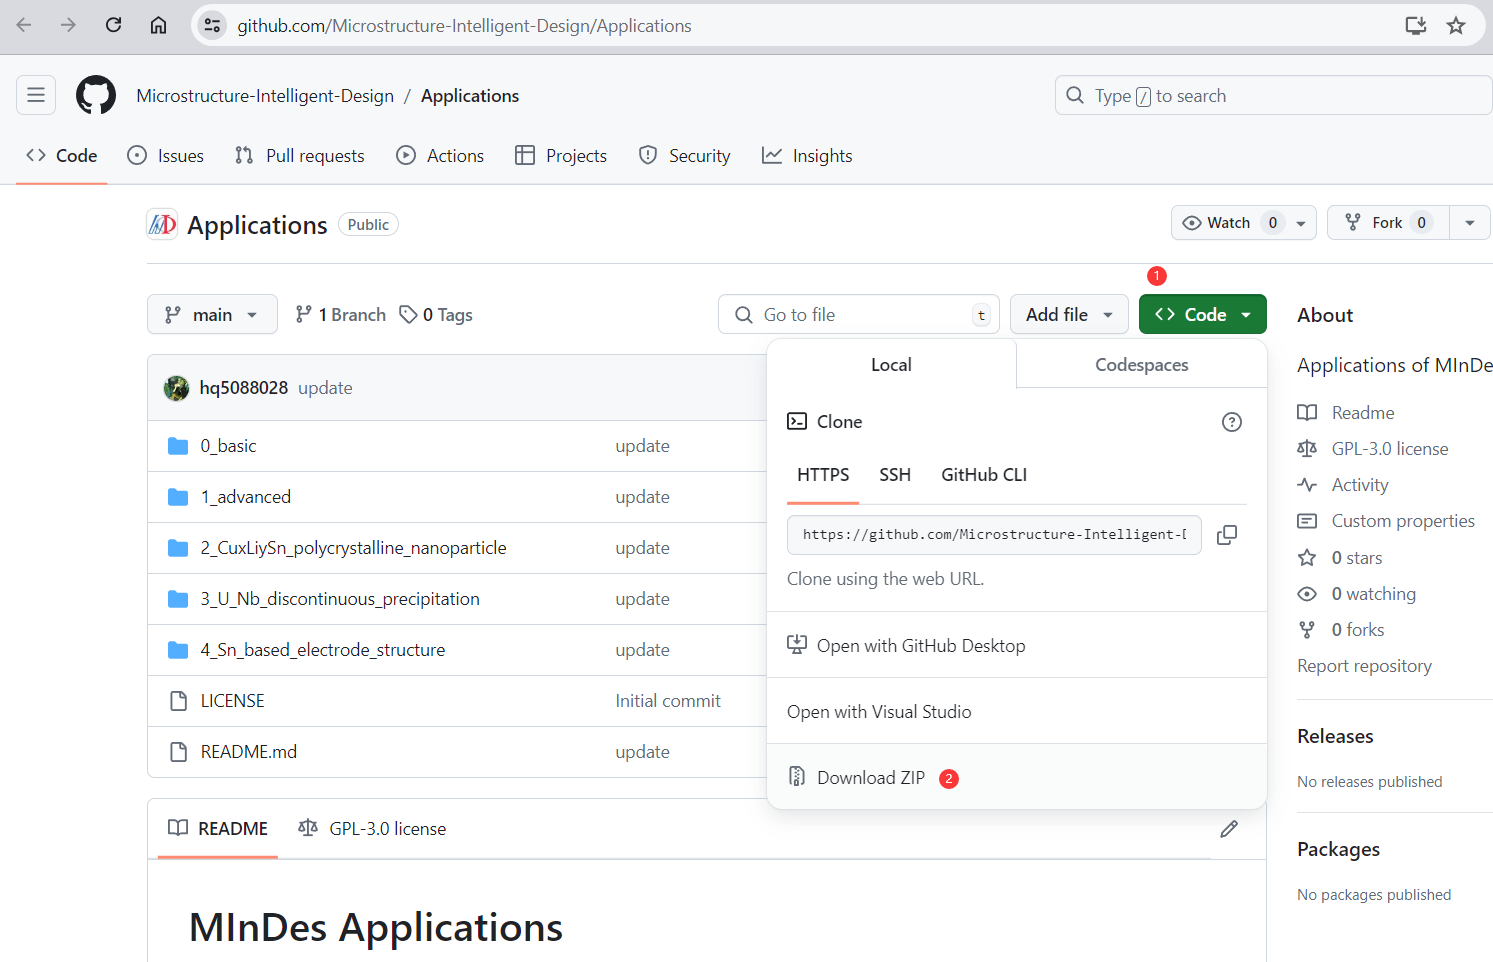
\includegraphics[width=5in]{rsc/download_mides.png}

随后将程序包解压缩,可得到以下文件:

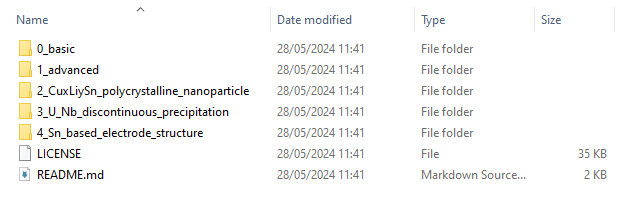
\includegraphics[width=5in]{rsc/mid_package_contents.png}

其中基本的输入文件位于文件夹 \emph{0\_basic} 中,其余应用案例位于后续文件夹中。
此处以 \emph{2\_CuxLiySn\_polycrystalline\_nanoparticle} 为例。

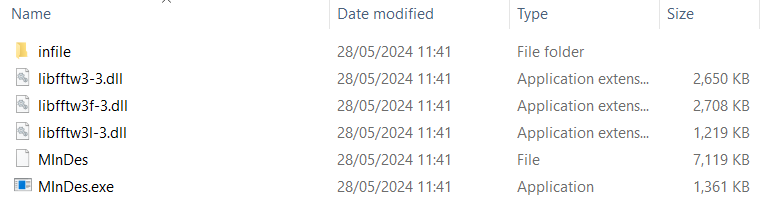
\includegraphics[width=5in]{rsc/example_folder.png}

自上而下分别为:\emph{infile}:输入文件所在文件夹;\emph{libfftw*.dll}:软件运行依赖;
\emph{MInDes}:Linix 系统执行程序;\emph{MInDes.exe}:Windows 系统执行程序。

于对应系统中运行可执行程序,即可进入软件配置界面:
\begin{itemize}
  \item {\color{magenta}Windows 环境下}:

        运行软件后键入\ \verb|i|\ 并回车,即可进入软件信息界面。\\
        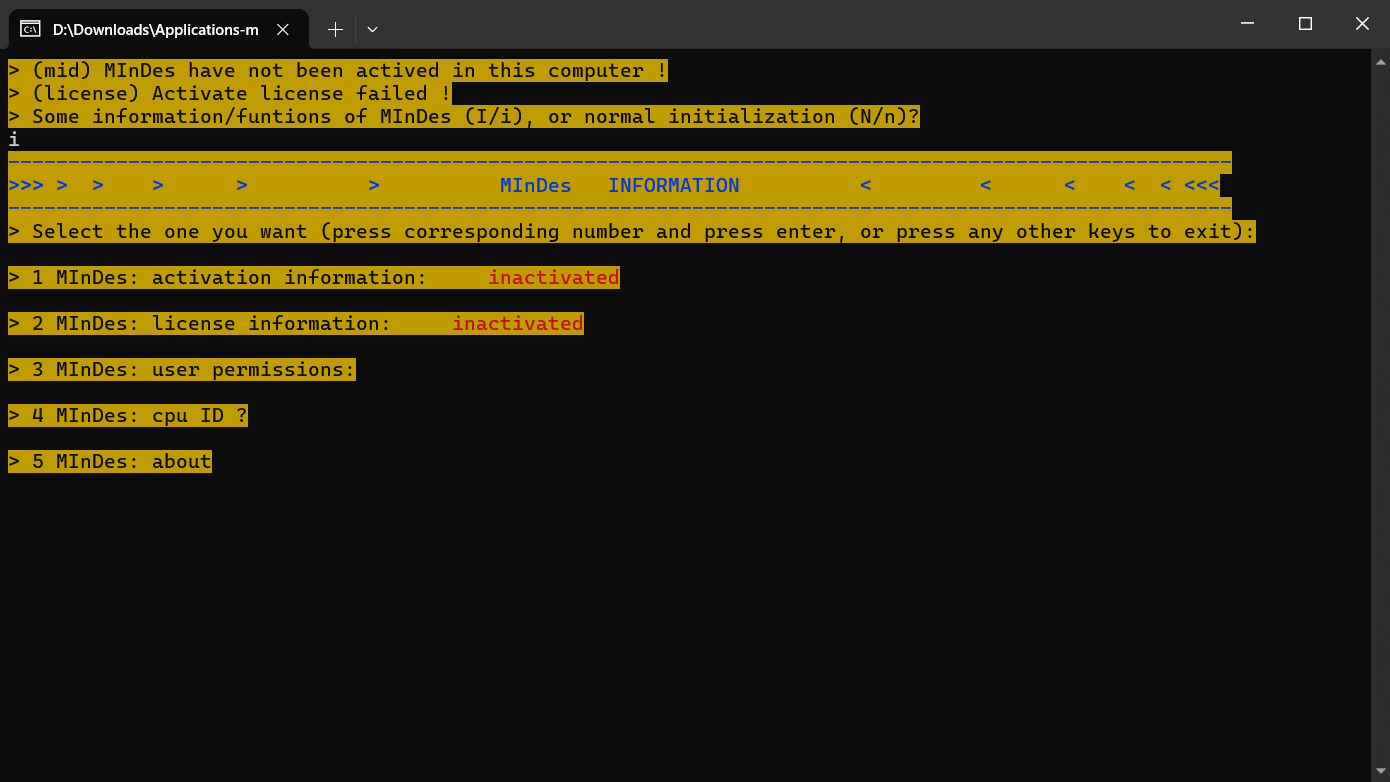
\includegraphics[width=5in]{rsc/mid_info_win.png}

  \item {\color{magenta}Linux 环境下}:

        无参数运行软件后将直接进入软件信息界面。\\
        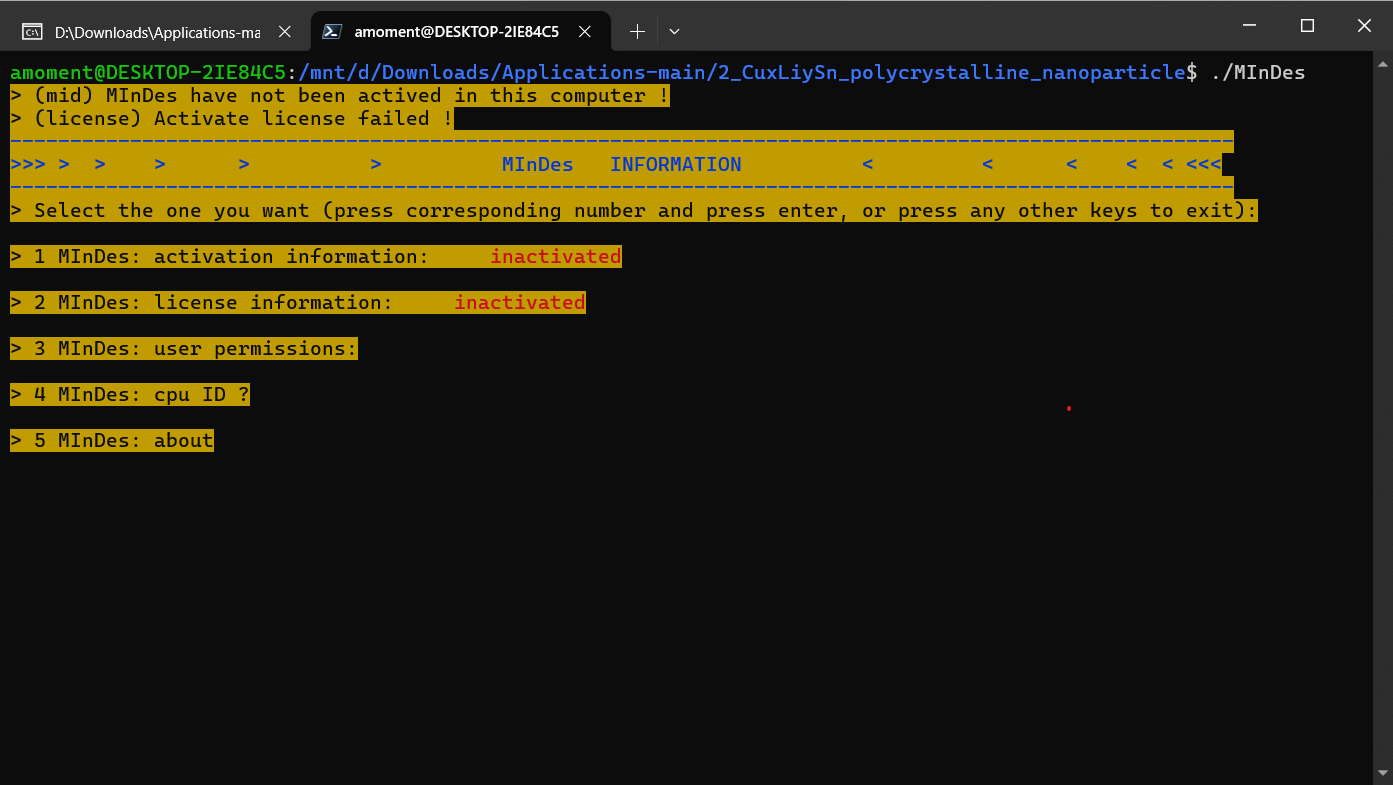
\includegraphics[width=5in]{rsc/mid_info_linux.png}

\end{itemize}
于此界面下,可以查看:(1)激活信息;(2)许可证信息;
(3)查看当前软件权限;(4)获取CPU ID;(5)查看软件概况(如下图)。

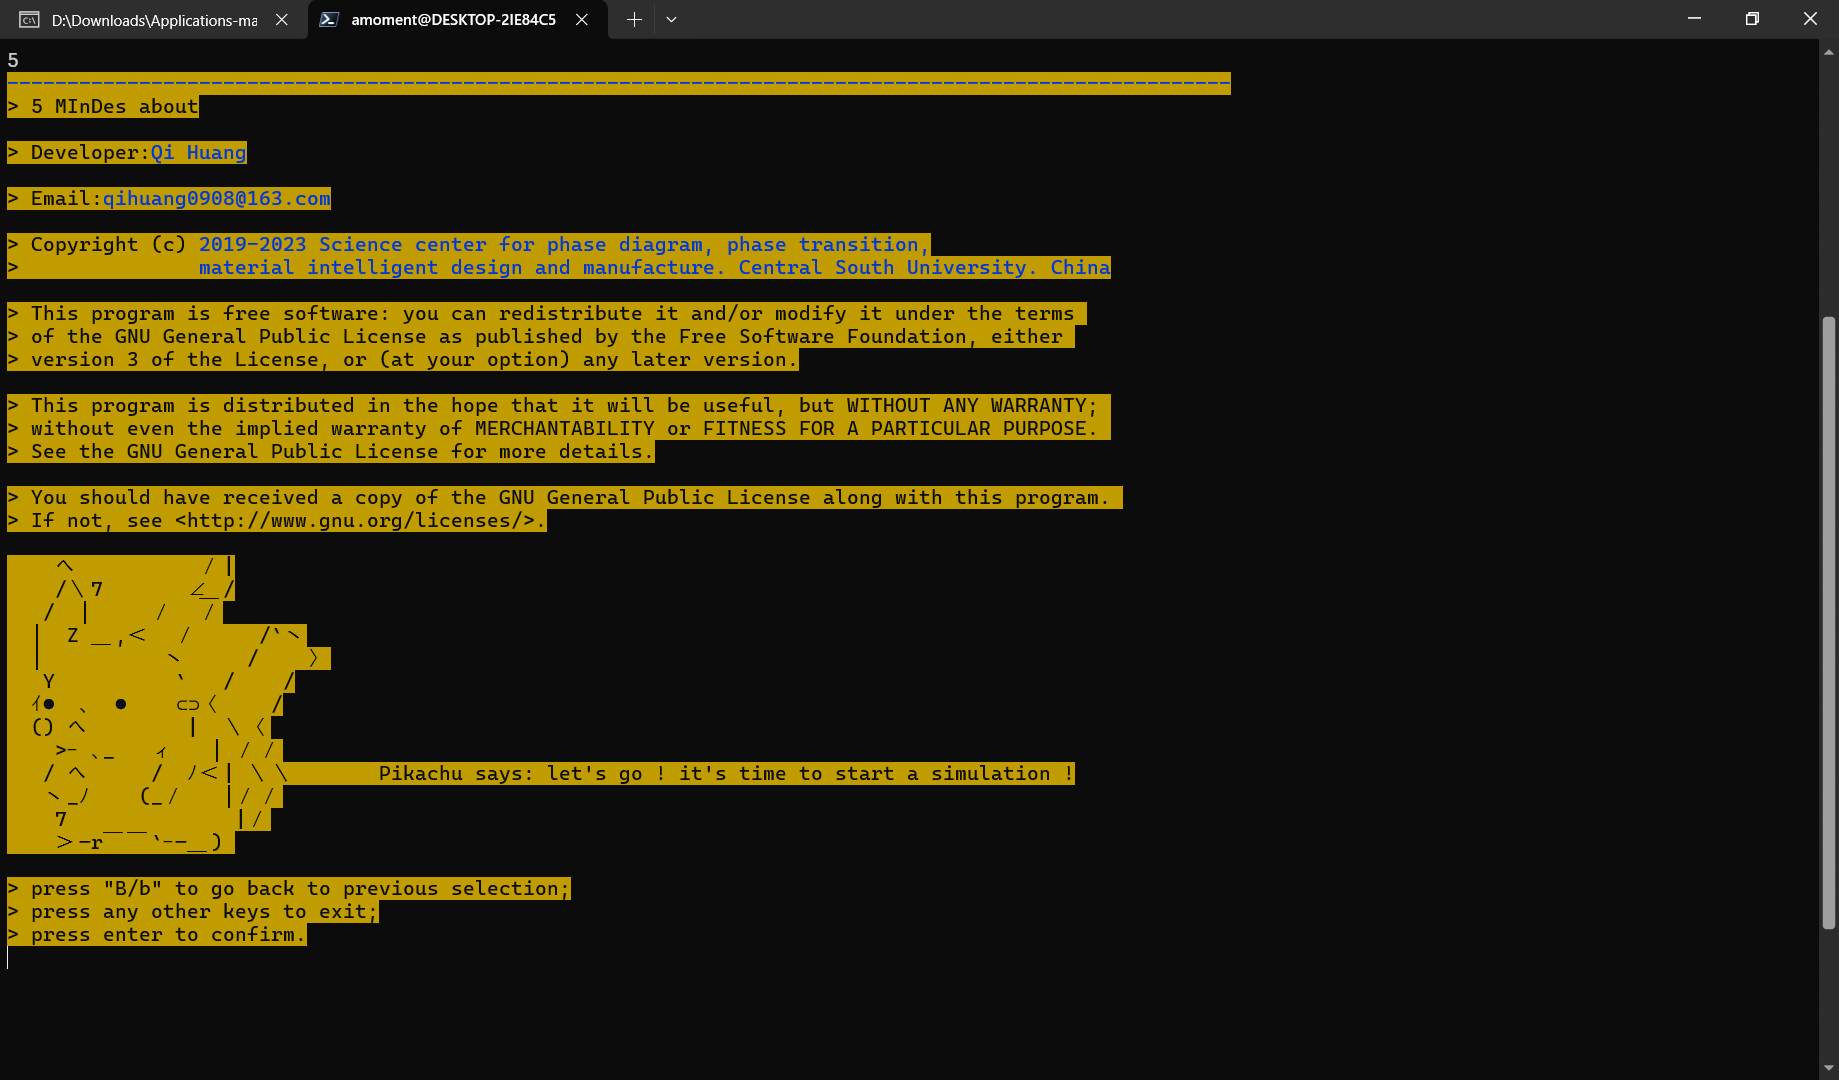
\includegraphics[width=5in]{rsc/mid_info_about.png}

\endinput

\chapter{MInDes 使用及示例}\label{chap:quick_start}



\endinput
\chapter{MInDes 输入文件(infile)}\label{chap:infile}


\endinput
\chapter{MInDes 输出结果}\label{chap:outputs}


\endinput
\chapter{MInDes 常见问题}\label{chap:faq}


\endinput
% \chapter{排版样式设定}\label{chap:styles}
\addtocontents{los}{\protect\addvspace{10pt}}

\begin{intro}
至此你已经基本学会排版内容丰富的文档,标题、目录、章节、公式、列表、图片、表格等等应有尽有。但是你可能已经有点不甘心了,
因为似乎你排版出来的文档是千篇一律的模样——\LaTeX{} 默认的字体、单调的页眉页脚、不太令你满意的页边距,等等。
本章的内容将带你一览如何修改 \LaTeX{} 的排版样式。
\end{intro}

\section{字体和字号}\label{sec:font}

\LaTeX{} 根据文档的逻辑结构(章节、脚注等)来选择默认的字体样式以及字号。
需要更改字体样式或字号的话,可以使用表 \ref{tbl:fonts} 和表 \ref{tbl:sizes} 中列出的命令。
\begin{example}
{\small The small and
\textbf{bold} Romans ruled}
{\Large all of great big
{\itshape Italy}.}
\end{example}

\LaTeXe{} 相比于较早的 \LaTeX{} 版本(2.09版或更早)在字体样式和字号的设定上有很大改进,令字体的各种属性相互独立(“正交”),
用户可以改变字体的大小,而仍然保留字体原有的粗体或者斜体的特性。

\subsection{字体样式}\label{subsec:fontshape}

\pinyinindex{ziti}{字体}
\pinyinindex{fenzu}{分组}
\LaTeX{} 提供了两组修改字体的命令,见表 \ref{tbl:fonts}。其中诸如 \cmd{bfseries} 形式的命令将会影响之后所有的字符,
如果想要让它在局部生效,需要用花括号\textbf{分组},也就是写成 \marg*{\cmd{bfseries}\ \Arg{some text}} 这样的形式;
对应的 \cmd{textbf} 形式带一个参数,只改变参数内部的字体,更为常用。

在公式中,直接使用 \cmd{textbf} 等命令不会起效,甚至报错。\LaTeX{} 提供了修改数学字母样式的命令,如 \cmd{mathbf} 等,详见 \ref{subsec:math-alpha} 小节。

\begin{table}[htp]
\caption{字体命令} \label{tbl:fonts}
\centering
\begin{tabular}{*{4}{l}}
\hline
\cmd{rmfamily}\cmdindex{rmfamily}      & \cmd{textrm}\cmdindex{textrm}\marg*{\ldots}           & \textrm{roman}           & 衬线字体(罗马体)\\
\cmd{sffamily}\cmdindex{sffamily}      & \cmd{textsf}\cmdindex{textsf}\marg*{\ldots}           & \textsf{sans serif}      & 无衬线字体        \\
\cmd{ttfamily}\cmdindex{ttfamily}      & \cmd{texttt}\cmdindex{texttt}\marg*{\ldots}           & \texttt{typewriter}      & 等宽字体          \\[\medskipamount]
\cmd{mdseries}\cmdindex{mdseries}      & \cmd{textmd}\cmdindex{textmd}\marg*{\ldots}           & \textrm{medium}          & 正常粗细(中等)  \\
\cmd{bfseries}\cmdindex{bfseries}      & \cmd{textbf}\cmdindex{textbf}\marg*{\ldots}           & \textbf{bold face}       & 粗体              \\[\medskipamount]
\cmd{upshape}\cmdindex{upshape}        & \cmd{textup}\cmdindex{textup}\marg*{\ldots}           & \textup{upright}         & 直立体            \\
\cmd{itshape}\cmdindex{itshape}        & \cmd{textit}\cmdindex{textit}\marg*{\ldots}           & \textit{italic}          & 意大利斜体        \\
\cmd{slshape}\cmdindex{slshape}        & \cmd{textsl}\cmdindex{textsl}\marg*{\ldots}           & \textsl{slanted}         & 倾斜体            \\
\cmd{scshape}\cmdindex{scshape}        & \cmd{textsc}\cmdindex{textsc}\marg*{\ldots}           & \textsc{Small Caps}      & 小型大写字母      \\[\medskipamount]
\cmd{em}\cmdindex{em}                  & \cmd{emph}\cmdindex{emph}\marg*{\ldots}               & \emph{emphasized}        & 强调,默认斜体    \\
\cmd{normalfont}\cmdindex{normalfont}  & \cmd{textnormal}\cmdindex{textnormal}\marg*{\ldots}   & \textnormal{normal font} & 默认字体          \\
\hline
\end{tabular}
\end{table}

\subsection{字号}\label{subsec:fontsize}

\pinyinindex{zihao}{字号}
字号命令实际大小依赖于所使用的文档类及其选项。表 \ref{tbl:ptsizes} 列出了这些命令在标准文档类中的绝对大小,单位为 pt。

\begin{table}[htp]
\centering
\caption{字号} \label{tbl:sizes}
\begin{tabular}{ll}
\hline
\cmd{tiny}\cmdindex{tiny}         & \tiny        tiny font \\
\cmd{scriptsize}\cmdindex{scriptsize}   & \scriptsize  very small font\\
\cmd{footnotesize}\cmdindex{footnotesize} & \footnotesize  quite small font \\
\cmd{small}\cmdindex{small}        &  \small            small font \\
\cmd{normalsize}\cmdindex{normalsize}   &  \normalsize  normal font \\
\cmd{large}\cmdindex{large}        &  \large       large font \\
\hline
\end{tabular}%
\qquad\begin{tabular}{ll@{}}
\hline
\cmd{Large}\cmdindex{Large}        &  \Large       larger font \\[5pt]
\cmd{LARGE}\cmdindex{LARGE}        &  \LARGE       very large font \\[5pt]
\cmd{huge}\cmdindex{huge}         &  \huge        huge \\[5pt]
\cmd{Huge}\cmdindex{Huge}         &  \Huge        largest \\
\hline
\end{tabular}
\end{table}

\begin{table}[htp]
\centering
\caption{标准文档类中的字号大小}\label{tbl:ptsizes}
\begin{tabular}{*{4}{l}}
\hline
\textbf{字号} & \textbf{10pt 选项(默认)} & \textbf{11pt 选项} & \textbf{12pt 选项} \\
\hline
\cmd{tiny}\cmdindex{tiny}       & 5pt  & 6pt & 6pt\\
\cmd{scriptsize}\cmdindex{scriptsize} & 7pt  & 8pt & 8pt\\
\cmd{footnotesize}\cmdindex{footnotesize} & 8pt & 9pt & 10pt \\
\cmd{small}\cmdindex{small}        & 9pt & 10pt & 10.95pt \\
\cmd{normalsize}\cmdindex{normalsize} & 10pt & 10.95pt & 12pt \\
\cmd{large}\cmdindex{large}      & 12pt & 12pt & 14.4pt \\
\cmd{Large}\cmdindex{Large}      & 14.4pt & 14.4pt & 17.28pt \\
\cmd{LARGE}\cmdindex{LARGE}      & 17.28pt & 17.28pt & 20.74pt\\
\cmd{huge}\cmdindex{huge}       & 20.74pt & 20.74pt & 24.88pt\\
\cmd{Huge}\cmdindex{Huge}       & 24.88pt & 24.88pt & 24.88pt\\
\hline
\end{tabular}
\end{table}

使用字号命令的时候,通常也需要用花括号进行分组,如同 \cmd{rmfamily} 那样。
\begin{example}
He likes {\LARGE large and
{\small small} letters}.
\end{example}

\cmdindex{fontsize}
\LaTeX{} 还提供了一个基础的命令 \cmd{fontsize} 用于设定任意大小的字号:
\begin{command}
\cmd{fontsize}\marg{size}\marg{base line-skip}
\end{command}

\cmdindex{selectfont}
\cmd{fontsize} 用到两个参数,\Arg{size} 为字号,\Arg{base line-skip} 为基础行距。
表 \ref{tbl:ptsizes} 中的命令也都各自设定了与字号对应的基础行距,大小为字号的 1.2 倍。
如果不是在导言区,\cmd{fontsize} 的设定需要 \cmd{selectfont} 命令才能立即生效,
而表 \ref{tbl:sizes} 的字号设定都是立即生效的。

\subsection{选用字体宏包}\label{subsec:font-pkgs}

至此已经介绍了如何改变字体样式如粗体、斜体等等,以及如何改变字号,
但你依然用着 \LaTeX{} 默认的那套、由高德纳设计制作的 Computer Modern 字体。
有的人可能很喜欢 Times / Palatino,或者更好看的字体。这些字体样式的自由设置在 \LaTeX{} 里还不太容易。

幸好大部分时候,许多字体宏包为我们完成了整套配置,我们可以在调用宏包之后,照常使用 \cmd{bfseries} 或 \cmd{ttfamily} 等我们熟悉的命令。
表 \ref{tbl:font-pkgs} 列出了较为常用的字体宏包,其中相当多的宏包还配置了数学字体,或者文本、数学字体兼而有之。
更多的字体配置参考 \cite{survey,fontcatalogue}。

\subsection{字体编码}\label{subsec:font-encs}

字体编码对于 \LaTeX{} 用户来讲是一个比较晦涩的概念。它规定了一个字体里包含的符号,并将若干符号用 \LaTeX{} 命令定义。
注意字体编码与我们在 \ref{subsec:ascii} 等小节叙述的 ASCII 编码等并非一一对应。

常见的正文字体编码有 \texttt{OT1} 和 \texttt{T1} 等。\LaTeX{} 默认使用兼容 \hologo{plainTeX} 的 \texttt{OT1} 编码,使用起来有诸多限制:
高德纳在设计 Computer Modern 字体时认为一些符号,如大于号、小于号等,原则上都应该在公式里出现,所以在正文字体里这些符号所在的位置被其它符号所占据
(\texttt{OT1} 字体编码、\cmd{rmfamily} 和 \cmd{sffamly} 字体族下, \texttt< 和 \texttt> 排版\ !` 和\ ?` 两个倒立的标点符号,
正常的大于号和小于号可用命令 \cmd{textgreater} 和 \cmd{textless} 输入;\cmd{ttfamily} 字体族下是正常的大于号和小于号)。
扩展的 \texttt{T1} 字体编码则更加靠近 ASCII 文本编码,不会出现上述的大于号、小于号的问题。

\pkgindex{fontenc}
切换字体编码要用到 \pkg{fontenc} 宏包:
\begin{command}
\cmd{usepackage}\oarg*{T1}\marg*{fontenc}
\end{command}

\pkg{fontenc} 宏包是用来配合传统的 \LaTeX{} 字体的,如表 \ref{tbl:font-pkgs} 中的一些传统字体宏包。如果使用 \texttt{xelatex} 编译方式,
并使用 \pkg{fontspec} 宏包调用 \texttt{ttf} 或 \texttt{otf} 格式字体,就不要再使用 \pkg{fontenc} 宏包。
使用表 \ref{tbl:font-pkgs} 中的字体宏包之前最好查看一下宏包的帮助文档,了解使用方法和注意事项。

\begin{table}[!p]
\centering\small
\caption{常见的 \LaTeX{} 字体宏包}\label{tbl:font-pkgs}
\begin{tabular}{lp{30em}}
 \hline
 \multicolumn{2}{c}{\textbf{文本/数学字体搭配的宏包}} \\
 \hline
 \pkg{lmodern}     & Latin Modern 字体,对 Computer Modern 字体的扩展  \\
 \pkg{cmbright}    & 仿 Computer Modern 风格的无衬线字体 \\
 \pkg{euler}       & Euler 风格数学字体,也出自于高德纳之手 \\
 \pkg{ccfonts}     & Concrete 风格字体 \\
 \pkg{txfonts}     & Times 风格的字体宏包  \\
 \pkg{pxfonts}     & Palatino 风格的字体宏包  \\
 \pkg{stix}        & Times 风格的字体宏包  \\
 \pkg{newtxtext},\pkg{newtxmath}  & \pkg{txfonts} 的改进版本,分别设置文本和数学字体  \\
 \pkg{newpxtext},\pkg{newpxmath}  & \pkg{pxfonts} 的改进版本,分别设置文本和数学字体  \\
 \pkg{mathptmx}    & \pkg{psnfss} 字体宏集之一,Times 风格,较为陈旧,不推荐使用  \\
 \pkg{mathpazo}    & \pkg{psnfss} 字体宏集之一,Palatino 风格,较为陈旧,不推荐使用  \\
 \pkg{fourier}     & Fourier 风格数学字体,配合 Utopia 正文字体 \\
 \pkg{fouriernc}   & Fourier 风格数学字体,配合 New Century Schoolbook 正文字体 \\
 \pkg{arev}        & Arev 无衬线字体宏包,Vera Sans 风格 \\
 \pkg{mathdesign}  & 配合 Charter / Garamond / Utopia 正文字体的数学字体宏包 \\
 \hline
 \multicolumn{2}{c}{\textbf{文本字体宏包}} \\
 \multicolumn{2}{l}{\footnotesize 以下字体包括传统的 \LaTeX{} 字体格式以及 TrueType / OpenType 格式。} \\
 \hline
 \pkg{cm-unicode}  & Computer Modern 风格的 Unicode 字体,支持多种西方语言 \\
 \pkg{dejavu}      & DejaVu 开源字体 \\
 \pkg{droid}       & Droid 开源字体 \\
 \pkg{inconsolata} & Inconsolata 开源等宽字体 \\
 \pkg{libertine}   & Linux Libertine / Linux Biolium 开源字体 \\
 \pkg{roboto}      & Roboto 开源无衬线字体 \\
 \pkg{sourcesanspro} & Source Sans Pro 开源无衬线字体 \\
 \pkg{sourcecodepro} & Source Code Pro 开源等宽字体 \\
 \hline
 \multicolumn{2}{c}{\textbf{符号宏包}} \\
 \hline
 \pkg{mathabx}     & 数学符号宏包之一 \\
 \pkg{MnSymbol}    & 数学符号宏包之一,配合 Minion Pro 文本字体  \\
 \pkg{fdsymbol}    & 数学符号宏包之一 \\
 \pkg{pifont}      & Zapf Dingbats 符号宏包 \\
 \hline
\end{tabular}
\end{table}

\subsection{使用 \pkg{fontspec} 宏包更改字体}\label{subsec:fontspec}

\index{xelatex@\texttt{xelatex} 命令}
\index{lualatex@\texttt{lualatex} 命令}
\texttt{xelatex} 和 \texttt{lualatex} 编译命令能够支持直接调用系统和 \TeX{} 发行版中的 \texttt{.ttf} 或 \texttt{.otf} 格式字体%
\footnote{Linux 下的 \hologo{TeXLive} 为了令 \hologo{XeTeX} 使用 OpenType 字体,需要额外的配置。详见附录 \ref{app:install}。}。
相比于前文介绍的字体宏包,我们有了更多自由修改字体的余地。

\pkgindex{fontspec}
\cmdindex[fontspec]{setmainfont,setsansfont,setmonofont}
\texttt{xelatex} 和 \texttt{lualatex} 命令下支持用户调用字体的宏包是 \pkg{fontspec}。
宏包提供了几个设置全局字体的命令,设置 \cmd{rmfamily} 等对应命令的默认字体%
\footnote{旧版本 \pkg{fontspec} 的命令把必选参数 \Arg{font name} 放在可选参数 \Arg{font features} 的后面。新版本目前兼容旧版本的用法,但推荐使用新版本的用法。}:
\begin{command}
\cmd{setmainfont}\marg{font name}\oarg{font features} \\
\cmd{setsansfont}\marg{font name}\oarg{font features} \\
\cmd{setmonofont}\marg{font name}\oarg{font features}
\end{command}
其中 \Arg{font name} 使用字体的文件名(带扩展名)或者字体的英文名称。\Arg{font features} 用来
手动配置对应的粗体或斜体,比如为 Windows 下的无衬线字体 Arial 配置粗体和斜体(通常情况下自动检测
并设置对应的粗体和斜体,无需手动指定):
\begin{verbatim}
\setsansfont{Arial}[BoldFont={Arial Bold}, ItalicFont={Arial Italic}]
\end{verbatim}
\Arg{font features} 还能配置字体本身的各种特性,这里不再赘述,感兴趣的读者请参考 \pkg{fontspec} 宏包的帮助文档。

需要注意的是,\pkg{fontspec} 宏包会覆盖数学字体设置。需要调用表 \ref{tbl:font-pkgs} 中列出的一些数学字体宏包时,
应当在调用 \pkg{fontspec} 宏包时指定 \texttt{no-math} 选项。\pkg{fontspec} 宏包可能被其它宏包或文档类(如 \pkg{ctex} 文档类)自动调用时,
则在文档开头的 \cmd{document\-class} 命令里指定 \texttt{no-math} 选项。

\subsection{在 \pkg{ctex} 宏包或文档类中更改中文字体}\label{subsec:CJKfont}

\pkgindex{xeCJK,ctex}
\cmdindex[xeCJK,ctex]{setCJKmainfont,setCJKsansfont,setCJKmonofont}
前文已经介绍过的 \pkg{ctex} 宏包或文档类提供了和 \pkg{fontspec} 宏包非常类似的语法设置中文字体%
\footnote{使用 \texttt{xelatex} 编译时,这几个命令实际上由 \pkg{xeCJK} 宏包提供;
使用 \texttt{lualatex} 编译时,则是由 \pkg{ctex} 宏包或文档类对 \pkg{luatexja} 宏包提供的类似命令进行额外封装。}:
\begin{command}
\cmd{setCJKmainfont}\marg{font name}\oarg{font features} \\
\cmd{setCJKsansfont}\marg{font name}\oarg{font features} \\
\cmd{setCJKmonofont}\marg{font name}\oarg{font features}
\end{command}

由于中文字体少有对应的粗体或斜体,\Arg{font features} 里多用其他字体来配置,
比如在 Windows 中设定基本字体为宋体,并设定对应的 \texttt{BoldFont} 为黑体, \texttt{ItalicFont} 为楷体:
\begin{verbatim}
\setCJKmainfont{SimSun}[BoldFont=SimHei, ItalicFont=KaiTi]
\end{verbatim}

\subsection{使用 \pkg{unicode-math} 宏包配置 Unicode 数学字体}\label{subsec:unicode-math}

\pkgindex{unicode-math}
\cmdindex[unicode-math]{setmathfont}
Unicode 数学字体是一类 OpenType 字体,包含了 Unicode 字符集中的数学符号部分,字体中也设定了数学公式排版所需的一些参数。在 \texttt{xelatex} 或者 \texttt{lualatex} 编译命令下,借助 \pkg{unicode-math} 宏包可以调用 Unicode 数学字体配置数学公式的字体风格。

在导言区使用 \cmd{usepackage}\marg*{unicode-math} 后,使用 \cmd{setmathfont} 命令即可:
\begin{command}
\cmd{setmathfont}\marg{font name}\oarg{font features}
\end{command}

绝大多数时候,只需要给定字体名称 \Arg{font name} 即可。由于篇幅所限,在此不介绍可选参数 \Arg{font feature} 涉及的配置,有兴趣的读者请参考宏包的帮助文档。Unicode 数学字体相比于正文字体的选择余地不多。表 \ref{tbl:uni-math-fonts} 给出了较为常用的 Unicode 数学字体。

\begin{table}[htp]
\centering\small
\caption{常用 Unicode 数学字体。}
\label{tbl:uni-math-fonts}
\begin{tabular}{llp{20em}}
\hline
\textbf{数学字体名称} & \textbf{配套正文字体名称} & \textbf{备注} \\
\hline
\multicolumn{3}{c}{开源字体,发布于 CTAN} \\
\hline
Latin Modern Math     & Latin Modern     & 基于 Computer Modern 风格 \\
STIX Math             & STIX             & Times 风格 \\
XITS Math             & XITS             & 基于 STIX,Times 风格,有粗体 XITS Math Bold 可用 \\
TeX Gyre Pagella Math & TeX Gyre Pagella & Palatino 风格 \\
TeX Gyre Termes Math  & TeX Gyre Termes  & Times 风格 \\
TeX Gyre DejaVu Math  & DejaVu Serif     & DejaVu 风格 \\
Libertinus Math       & Libertinus       & Linux Libertine 风格 \\
Garamond Math         & EB Garamond      & Garamond 风格 \\
Fira Math             & Fira Sans        & 无衬线数学字体 \\
\hline
\multicolumn{3}{c}{商业字体} \\
\hline
Cambria Math          & Cambria          & 微软 Office 预装的数学字体 \\
Lucida Bright Math OT & Lucida Bright OT & 须购买商业授权 \\
Minion Math           & Minion Pro       & 须购买商业授权 \\
\hline
\end{tabular}
\end{table}

\pkg{unicode-math} 宏包与传统数学字体、符号包并不兼容,但其本身已经提供了大量的符号和字体样式。实际上,\ref{subsec:math-alpha} 和 \ref{subsec:math-bold} 小节中介绍的内容均已被 \pkg{unicode-math} 所涵盖,无需调用其他宏包就可以获得覆盖完整、风格较为统一的字体样式。具体使用方法请参考宏包帮助文档。

\section{文字装饰和强调}\label{sec:emphasize}

强调文字的方法,或者是添加下划线等装饰物,或者是改变文字的字体。

\cmdindex{underline}
\LaTeX{} 定义了 \cmd{underline} 命令用来为文字添加下划线:
\begin{example}
An \underline{underlined} text.
\end{example}

\pkgindex{ulem}
\cmdindex[ulem]{uline}
\cmd{underline} 命令生成下划线的样式不够灵活,不同的单词可能生成高低各异的下划线,并且无法换行。
\pkg{ulem} 宏包提供了更灵活的解决方案,它提供的 \cmd{uline} 命令能够轻松生成自动换行的下划线:
\begin{example}
An example of \uline{some
long and underlined words.}
\end{example}

\cmdindex{emph}
前一节介绍了 \cmd{emph} 命令,它将文字变为斜体以示强调,而如果在已强调的文字中嵌套使用 \cmd{emph} 命令,
命令内则使用直立体文字:
\begin{example}
Some \emph{emphasized words,
including \emph{double-emphasized}
words}, are shown here.
\end{example}

\section{段落格式和间距}\label{sec:par-lengths}

\subsection{长度和长度变量}\label{subsec:lengths}

在前面的一些章节,我们已经见到一些长度和长度变量的用法。本节首先统一介绍长度和长度变量。

长度的数值 \Arg{length} 由数字和单位组成。常用的单位见表 \ref{tbl:length-unit}。

\def\unitindex#1{\index{#1@\texttt{#1} (\textit{长度单位})}}

\begin{table}[htp]
\centering
\caption{\TeX{} / \LaTeX{} 中的长度单位}\label{tbl:length-unit}
\begin{tabular}{ll}
 \hline
 \texttt{pt}\unitindex{pt} & 点阵宽度,1/72.27\texttt{in} \\
 \texttt{bp}\unitindex{bp} & 点阵宽度,1/72\texttt{in} \\
 \texttt{in}\unitindex{in} & 英寸 \\
 \texttt{cm}\unitindex{cm} & 厘米 \\
 \texttt{mm}\unitindex{mm} & 毫米 \\
 \hline
 \texttt{em}\unitindex{em} & 当前字号下大写字母 M 的宽度,常用于水平距离的设定 \\
 \texttt{ex}\unitindex{ex} & 当前字号下小写字母 x 的高度,常用于垂直距离的设定 \\
 \hline
\end{tabular}
\end{table}

在一些情况下还会用到可伸缩的“弹性长度”,如 \texttt{12pt plus 2pt minus 3pt}
表示基础长度为 \texttt{12pt},可以伸展到 \texttt{14pt},也可以收缩到 \texttt{9pt}。
也可只定义 \texttt{plus} 或者 \texttt{minus} 的部分,如 \texttt{0pt plus 5pt}。

长度的数值还可以用长度变量本身或其倍数来表达,如 \texttt{2.5}\cmd{parindent} 等。

\cmdindex{newlength,setlength,addtolength}
\LaTeX{} 预定义了大量的长度变量用于控制版面格式。如页面宽度和高度、首行缩进、段落间距等。
如果需要自定义长度变量,需使用如下命令:
\begin{command}
\cmd{newlength}\marg*{\cmd{\Arg{length command}}}
\end{command}

长度变量可以用 \cmd{setlength} 赋值,或用 \cmd{addtolength} 增加长度:
\begin{command}
\cmd{setlength}\marg*{\cmd{\Arg{length command}}}\marg{length} \\
\cmd{addtolength}\marg*{\cmd{\Arg{length command}}}\marg{length}
\end{command}

\subsection{行距}\label{subsec:linespread}

\pinyinindex{hangju}{行距}
\cmdindex{linespread}
前文中我们提到过 \cmd{fontsize} 命令可以为字号设定对应的行距,但我们很少那么用。
更常用的办法是在导言区使用 \cmd{linespread} 命令。
\begin{command}
\cmd{linespread}\marg{factor}
\end{command}

其中 \Arg{factor} 作用于基础行距而不是字号。缺省的基础行距是 1.2 倍字号大小(参考 \cmd{font\-size} 命令),
因此使用 \cmd{line\-spread}\marg*{1.5} 意味着最终行距为 1.8 倍的字号大小。

\cmdindex{selectfont}
如果不是在导言区全局修改,而想要局部地改变某个段落的行距,需要用 \cmd{select\-font} 命令使 \cmd{line\-spread} 命令的改动立即生效:
\begin{example}
{\linespread{2.0}\selectfont
The baseline skip is set to be
twice the normal baseline skip.
Pay attention to the \verb|\par|
command at the end. \par}

In comparison, after the
curly brace has been closed,
everything is back to normal.
\end{example}

\cmdindex{par}
字号的改变是即时生效的,而行距的改变直到文字\textbf{分段}时才生效。
如果需要改变某一部分文字的行距,那么不能简单地将文字包含在花括号内。注意下面两个例子中 \cmd{par} 命令的位置,包括上一个例子的写法
(\cmd{par} 相当于分段,见 \ref{subsec:spaces} 小节):
\begin{example}
{\Large Don't read this!
 It is not true.
 You can believe me!\par}
\end{example}

\begin{example}
{\Large This is not true either.
But remember I am a liar.}\par
\end{example}

\subsection{段落格式}\label{subsec:par-shape}

以下长度分别为段落的左缩进、右缩进和首行缩进:
\begin{command}
\cmd{setlength}\marg*{\cmd{leftskip}}\marg{length}  \\
\cmd{setlength}\marg*{\cmd{rightskip}}\marg{length} \\
\cmd{setlength}\marg*{\cmd{parindent}}\marg{length}
\end{command}

它们和设置行距的命令一样,在分段时生效。

\cmdindex{indent,noindent}
控制段落缩进的命令为:

\begin{command}
\cmd{indent} \\
\cmd{noindent}
\end{command}

\LaTeX{} 默认在段落开始时缩进,长度为用上述命令设置的 \cmd{parindent}。如果需要在某一段不缩进,可在段落开头使用
\cmd{noindent} 命令。相反地,\cmd{indent} 命令强制开启一段首行缩进的段落。在段落开头使用多个 \cmd{indent} 命令可以累加缩进量。

\pkgindex{indentfirst}
\LaTeX{} 还默认\textbf{在 \cmd{chapter}、\cmd{section} 等章节标题命令之后的第一段不缩进}%
\footnote{\pkg{ctex} 宏包和文档类默认按照中文习惯保持标题后第一段的首行缩进。}。
如果不习惯这种设定,可以调用 \pkg{indent\-first} 宏包,令第一段的首行缩进照常。

\cmdindex{parskip}
段落间的垂直间距为 \cmd{parskip},如设置段落间距在 \texttt{0.8ex} 到 \texttt{1.5ex} 变动:
\begin{verbatim}
\setlength{\parskip}{1ex plus 0.5ex minus 0.2ex}
\end{verbatim}

\subsection{水平间距}\label{subsec:hspace}

\cmdindex{hspace}
\LaTeX{} 默认为将单词之间的“空格”转化为水平间距。如果需要在文中手动插入额外的水平间距,可使用 \cmd{hspace} 命令:
\begin{example}
This\hspace{1.5cm}is a space
of 1.5 cm.
\end{example}

\cmdindex{hspace*}
\cmd{hspace} 命令生成的水平间距如果位于一行的开头或末尾,则有可能因为断行而被舍弃。可使用 \cmd{hspace*} 命令代替 \cmd{hspace} 命令
得到不会因断行而消失的水平间距。

\cmdindex{stretch,fill}
命令 \cmd{stretch}\marg{n} 生成一个特殊弹性长度,参数 \Arg{n} 为权重。它的基础长度为 0pt,但可以无限延伸,直到占满可用的空间。
如果同一行内出现多个 \cmd{stretch}\marg{n},这一行的所有可用空间将按每个 \cmd{stretch} 命令给定的权重 \Arg{n} 进行分配。

命令 \cmd{fill} 相当于 \cmd{stretch}\marg*{1}%
\footnote{注意不要用 \texttt{1.5}\cmd{fill} 这样的用法,它生成的长度只有基础长度 0pt 而没有延伸部分。}。

\begin{example}
x\hspace{\stretch{1}}
x\hspace{\stretch{3}}
x\hspace{\fill}x
\end{example}

\cmdindex{quad,qquad}
在正文中用 \cmd{hspace} 命令生成水平间距时,往往使用 \texttt{em} 作为单位,生成的间距随字号大小而变。
我们在数学公式中见过 \cmd{quad} 和 \cmd{qquad} 命令,它们也可以用于文本中,分别相当于 \cmd{hspace}\marg*{1em} 和 \cmd{hspace}\marg*{2em}:

\begin{example}
{\Large big\hspace{1em}y}\\
{\Large big\quad y}\\
nor\hspace{2em}mal\\
nor\qquad mal\\
{\tiny tin\hspace{1em}y}\\
{\tiny tin\quad y}
\end{example}

\subsection{垂直间距}\label{subsec:vspace}

在页面中,段落、章节标题、行间公式、列表、浮动体等元素之间的间距是 \LaTeX{} 预设的。比如 \cmd{parskip},默认设置为 \texttt{0pt plus 1pt}。

\cmdindex{vspace,vspace*}
如果我们想要人为地增加段落之间的垂直间距,可以在两个段落之间的位置使用 \cmd{vspace} 命令:
\begin{example}
A paragraph.

\vspace{2ex}
Another paragraph.
\end{example}

\cmd{vspace} 命令生成的垂直间距在一页的顶端或底端可能被“吞掉”,类似 \cmd{hspace} 在一行的开头和末尾那样。
对应地,\cmd{vspace*} 命令产生不会因断页而消失的垂直间距。\cmd{vspace} 也可用 \cmd{stretch} 设置无限延伸的垂直长度。

\index{\@\crcmd{} (\textit{换行})}
在段落内的两行之间增加垂直间距,一般通过给断行命令 \crcmd{} 加可选参数,如 \crcmd\texttt{[6pt]} 或 \crcmd\texttt{*[6pt]}。
\cmd{vspace} 也可以在段落内使用,区别在于 \cmd{vspace} 只引入垂直间距而不断行:
\begin{example}
Use command \verb|\vspace{12pt}|
to add \vspace{12pt} some spaces
between lines in a paragraph.

Or you can use \verb|\\[12pt]|
to \\[12pt] add vertical space,
but it also breaks the line.
\end{example}

\cmdindex{bigskip,medskip,smallskip}
另外 \LaTeX{} 还提供了\cmd{bigskip}, \cmd{medskip}, \cmd{smallskip} 来增加预定义长度的垂直间距。
\begin{example}
\parbox[t]{3em}{TeX\par TeX}
\parbox[t]{3em}{TeX\par\smallskip TeX}
\parbox[t]{3em}{TeX\par\medskip TeX}
\parbox[t]{3em}{TeX\par\bigskip TeX}
\end{example}

\section{页面和分栏}\label{sec:page-columns}

我们不妨回顾一下第一章介绍的文档类属性。\LaTeX{} 允许用户通过为文档类指定选项来控制纸张的大小(见 \ref{subsec:classes} 小节),
包括 \texttt{a4paper}、\texttt{letterpaper}等等,并配合字号设置了适合的页边距。

\cmdindex{textheight,textwidth}
控制页边距的参数由图 \ref{fig:layouts} 里给出的各种长度变量控制。
可以用 \cmd{setlength} 命令修改这些长度变量,以达到调节页面尺寸和边距的作用;
反之也可以利用这些长度变量来决定排版内容的尺寸,如在 \env{tabularx} 环境或 \cmd{include\-graphics} 命令的参数里,
设置图片或表格的宽度为 0.8\cmd{textwidth}。

\begin{figure}[!p]
\centering
\layoutpicture*
\caption{本文档的页面参数示意图(奇数页;由 \pkg{layout} 宏包生成)。} \label{fig:layouts}
\end{figure}

页边距等比较直观的参数则必须间接设置。我们根据图 \ref{fig:layouts} 将各个方向的页边距计算公式给出(以奇数页为例):
\begin{align*}
\text{\Arg{left-margin}}   &= \text{\ttfamily 1in}
                            + \text{\cmd{hoffset}}
                            + \text{\cmd{oddsidemargin}} \\
\text{\Arg{right-margin}}  &= \text{\cmd{paperwidth}}
                            - \text{\Arg{left-margin}}
                            - \text{\cmd{textwidth}} \\
\text{\Arg{top-margin}}    &= \text{\ttfamily 1in}
                            + \text{\cmd{voffset}}
                            + \text{\cmd{topmargin}}
                            + \text{\cmd{headheight}}
                            + \text{\cmd{headsep}} \\
\text{\Arg{bottom-margin}} &= \text{\cmd{paperheight}}
                            - \text{\Arg{top-margin}}
                            - \text{\cmd{textheight}}
\end{align*}
如果需要设置合适的 \Arg{left-margin} 和 \Arg{right-margin},就要通过上述方程组把 \cmd{odd\-sidemargin} 和 \cmd{text\-width} 等参数解出来!

幸好 \pkg{geometry} 宏包提供了设置页边距等参数的简便方法,能够帮我们完成背后繁杂的计算。

\subsection{利用 \pkg{geometry} 宏包设置页面参数}\label{subsec:geometry}

\pkgindex{geometry}
\pinyinindex{xuanxiang}{选项(宏包/文档类)}
\pkg{geometry} 宏包的调用方式类似于 \pkg{graphicx},在 \texttt{latex} + \texttt{dvipdfmx} 命令下
需要指定选项 \texttt{dvipdfm} 或 \texttt{dvipdfmx}%
\footnote{早期版本的 \pkg{geometry} 宏包仅支持 \texttt{dvipdfm} 选项。};
\texttt{pdflatex} 和 \texttt{xelatex} 编译命令下不需要。

\cmdindex[geometry]{geometry}
既可以调用 \pkg{geometry} 宏包,然后用其提供的 \cmd{geometry} 命令设置页面参数:
\begin{command}
\cmd{usepackage}\marg*{geometry} \\
\cmd{geometry}\marg{geometry-settings}
\end{command}
也可以直接在宏包选项中设置:
\begin{command}
\cmd{usepackage}\oarg{geometry-settings}\marg*{geometry}
\end{command}
其中 \Arg{geometry-settings} 多以 \Arg{key}=\Arg{value} 的形式组织。

比如,符合 Microsoft Word 习惯的页面设定是 A4 纸张,上下边距 1 英寸,左右边距 1.25 英寸,于是我们
可以通过如下两种等效的方式之一设定页边距:
\begin{verbatim}
\geometry{a4paper,left=1.25in,right=1.25in,top=1in,bottom=1in}
% or like this:
\geometry{a4paper,hmargin=1.25in,vmargin=1in}
\end{verbatim}

又比如,需要设定周围的边距一致为 1.25 英寸,可以用更简单的语法:
\begin{verbatim}
\geometry{margin=1.25in}
\end{verbatim}

对于书籍等双面文档,习惯上奇数页右边、偶数页左边留出较大的页边距,而靠近书脊一侧的奇数页左边、
偶数页右边页边距较小。我们可以这样设定:
\begin{verbatim}
\geometry{inner=1in,outer=1.25in}
\end{verbatim}

需要指出的是,通过 \pkg{geometry} 宏包设置的纸张大小是输出 PDF 文件的真实大小,而在文档类选项中
设置的参数(见 \ref{subsec:classes} 小节)实际上只影响输出区域。\pkg{geometry} 宏包还能够修改
页眉页脚高度、边注宽度等参数,并且能比较好地处理各参数之间的依赖关系。更详细的用法不再赘述,感兴趣
的用户可查阅其帮助文档。

\subsection{页面内容的垂直对齐}\label{subsec:raggedbottom}

\LaTeX{} 默认将页面内容在垂直方向分散对齐。对于有大量图表的文档,许多时候想要做到排版匀称的页面
很困难,垂直分散对齐会造成某些页面的垂直间距过宽,还可能报大量的 \verb|Underfull \vbox| 警告。
\LaTeX{} 还提供了另一种策略:将页面内容向顶部对齐,给底部留出高度不一的空白。

\cmdindex{raggedbottom, flushbottom}
以下命令分别令页面在垂直方向向顶部对齐/分散对齐:
\begin{command}
\cmd{raggedbottom} \\
\cmd{flushbottom}
\end{command}

\subsection{分栏}\label{subsec:columns}

\cmdindex{onecolumn,twocolumn}
\LaTeX{} 支持简单的单栏或双栏排版。标准文档类的全局选项 \texttt{onecolumn}、\texttt{twocolumn}
可控制全文分单栏或双栏排版。\LaTeX{} 也提供了切换单/双栏排版的命令:
\begin{command}
\cmd{onecolumn} \\
\cmd{twocolumn}\oarg{one-column top material}
\end{command}

\cmd{twocolumn} 支持带一个可选参数,用于排版双栏之上的一部分单栏内容。

\cmdindex{newpage,clearpage}
切换单/双栏排版时总是会另起一页(\cmd{clearpage})。
在双栏模式下使用 \cmd{newpage} 会换栏而不是换页;\cmd{clearpage} 则能够换页。

\cmdindex{columnwidth,columnsep,columnseprule}
双栏排版时每一栏的宽度为 \cmd{columnwidth},它由 \cmd{textwidth} 减去 \cmd{columnsep} 的差除以 2 得到。
两栏之间还有一道竖线,宽度为 \cmd{columnseprule},默认为零,也就是看不到竖线。

\pkgindex{multicol}
\envindex[multicol]{multicols}
一个比较好用的分栏解决方案是 \pkg{multicol},它提供了简单的 \env{multicols} 环境
(注意不要写成 \env{multicol} 环境)自动产生分栏,如以下环境将内容分为 3 栏:
\begin{verbatim}
\begin{multicols}{3}
...
\end{multicols}
\end{verbatim}

\pinyinindex{fudongti}{浮动体}
\envindex{table,figure}
\pkgindex{float}
\pkg{multicol} 宏包能够在一页之中切换单栏/多栏,也能处理跨页的分栏,且各栏的高度分布平衡。但代价是%
\textbf{在 \env{multicols} 环境中无法正常使用 \env{table} 和 \env{figure} 等浮动体环境},它会直接让浮动体丢失。
\env{multicols} 环境中只能用跨栏的 \env{table*} 和 \env{figure*} 环境,或者用 \pkg{float} 宏包提供的 \texttt{H} 参数固定浮动体的位置。

\section{页眉页脚}\label{sec:pagestyle}

\subsection{基本的页眉页脚样式}\label{subsec:basic-pagesyle}

\cmdindex{pagestyle,thispagestyle}
\pinyinindex{yemei}{页眉}
\pinyinindex{yejiao}{页脚}
\LaTeX{} 中提供了命令 \cmd{pagestyle} 来修改页眉页脚的样式:
\begin{command}
\cmd{pagestyle}\marg{page-style}
\end{command}

命令 \cmd{thispagestyle} 只影响当页的页眉页脚样式:
\begin{command}
\cmd{thispagestyle}\marg{page-style}
\end{command}

\Arg{page-style} 参数为样式的名称,在 \LaTeX{} 里预定义了四类样式,见表 \ref{tbl:pagestyle}。

\begin{table}[htp]
\centering
\caption{\LaTeX{} 预定义的页眉页脚样式}\label{tbl:pagestyle}
\begin{tabular}{lp{30em}}
 \hline
 \texttt{empty}  & 页眉页脚为空 \\
 \texttt{plain}  & 页眉为空,页脚为页码。(\cls{article} 和 \cls{report} 文档类默认;\cls{book} 文档类的每章第一页也为 plain 格式) \\
 \hline
 \texttt{headings}  & 页眉为章节标题和页码,页脚为空。(\cls{book} 文档类默认) \\
 \texttt{myheadings}  & 页眉为页码及 \cmd{markboth} 和 \cmd{markright} 命令手动指定的内容,页脚为空。\\
 \hline
\end{tabular}
\end{table}

\clsindex{article,report,book}
其中 \texttt{headings} 的情况较为复杂:
\begin{description}
  \item[\cls{article} 文档类,\texttt{twoside} 选项] 偶数页为页码和节标题,奇数页为小节标题和页码;
  \item[\cls{article} 文档类,\texttt{oneside} 选项] 页眉为节标题和页码;
  \item[\cls{report} / \cls{book} 文档类,\texttt{twoside} 选项] 偶数页为页码和章标题,奇数页为节标题和页码;
  \item[\cls{report} / \cls{book} 文档类,\texttt{oneside} 选项] 页眉为章标题和页码。
\end{description}

\cmdindex{pagenumbering}
\cmd{pagenumbering} 命令令我们能够改变页眉页脚中的页码样式:
\begin{command}
\cmd{pagenumbering}\marg{style}
\end{command}

\cmdindex{frontmatter,mainmatter}
\Arg{style} 为页码样式,默认为 \texttt{arabic}(阿拉伯数字),还可修改为 \texttt{roman}(小写罗马数字)、
\texttt{Roman}(大写罗马数字)等。注意使用 \cmd{pagenumbering} 命令后会将页码重置为 1。\cls{book} 文档类的 \cmd{front\-matter} 和 \cmd{main\-matter} 内部就使用了 \cmd{page\-numbering} 命令切换页码样式。
对页码格式的详细说明见 \ref{sec:counters} 节。

\subsection{手动更改页眉页脚的内容}\label{subsec:marks}

\cmdindex{markright,markboth}
对于 headings 或者 myheadings 样式,\LaTeX{} 允许用户使用命令手动修改页眉上面的内容,
特别是因为使用了 \cmd{chapter*} 等命令而无法自动生成页眉页脚的情况:
\begin{command}
\cmd{markright}\marg{right-mark}\\
\cmd{markboth}\marg{left-mark}\marg{right-mark}
\end{command}

在双面排版、\texttt{headings / myheadings} 页眉页脚样式下,\Arg{left-mark} 和 \Arg{right-mark} 的内容分别预期出现在左页(偶数页)和右页(奇数页)。
事实上 \cmd{chapter} 和 \cmd{section} 等章节命令内部也使用 \cmd{mark\-both} 或者 \cmd{mark\-right} 生成页眉。

\LaTeX{} 默认将页眉的内容都转为大写字母。如果需要保持字母的大小写,可以尝试以下代码
(\cmd{\renewcommand} 命令的用法详见 \ref{subsec:newcmd} 节)%
\footnote{但是这不能改变页眉的斜体样式(\cmd{slshape}),斜体是定义在 \texttt{headings} 样式里的。
如果不喜欢斜体,可在 \cmd{mark\-both} 等命令的参数里先使用 \cmd{normal\-font},再使用想要的字体样式命令,
或直接尝试使用 \pkg{fancyhdr} 宏包。}:
\begin{verbatim}
\renewcommand\chaptermark[1]{%
  \markboth{Chapter \thechapter\quad #1}{}}
\renewcommand\sectionmark[1]{%
  \markright{\thesection\quad #1}}
\end{verbatim}

其中 \cmd{thechapter}、\cmd{thesection} 等命令为章节计数器的数值(详见 \ref{sec:counters} 节)。以上代码适用于 \cls{report} / \cls{book} 文档类。
对于 \cls{article} 文档类,与两个页眉相关的命令分别为 \cmd{sec\-tion\-mark} 和 \cmd{sub\-sec\-tion\-mark}。

\subsection{\pkg{fancyhdr} 宏包}\label{subsec:fancyhdr}

\pkgindex{fancyhdr}
\pkg{fancyhdr} 宏包改善了页眉页脚样式的定义方式,允许我们将内容自由安置在页眉和页脚的左、中、右三个位置,还为页眉和页脚各加了一条横线。

\cmdindex[fancyhdr]{fancyhead,fancyfoot,fancyhf}
\pkg{fancyhdr} 自定义了样式名称 \texttt{fancy}。使用 \pkg{fancyhdr} 宏包定义页眉页脚之前,通常先用 \cmd{page\-style}\marg*{fancy} 调用这个样式。
在 \pkg{fancyhdr} 中定义页眉页脚的命令为:
\begin{command}
\cmd{fancyhf}\oarg{position}\marg*{\ldots}\\
\cmd{fancyhead}\oarg{position}\marg*{\ldots}\\
\cmd{fancyfoot}\oarg{position}\marg*{\ldots}
\end{command}
其中 \Arg{position} 为 L(左)/C(中)/R(右)以及与 O(奇数页)/E(偶数页)字母的组合。\cmd{fancyhf} 用于同时定义页眉和页脚,
习惯上使用 \cmd{fancyhf}\marg*{} 来清空页眉页脚的设置。

源代码 \ref{code:fancyhdr} 给出了 \pkg{fancyhdr} 基础用法的一个示例,效果为将章节标题放在和 headings 一致的位置,但使用加粗格式;
页码都放在页脚正中;修改横线宽度,“去掉”页脚的横线。

\begin{sourcecode}[htp]
  \begin{Verbatim}
  % 在导言区使用此代码
  \usepackage{fancyhdr}
  \pagestyle{fancy}
  \renewcommand{\chaptermark}[1]{\markboth{#1}{}}
  \renewcommand{\sectionmark}[1]{\markright{\thesection\ #1}}
  \fancyhf{}
  \fancyfoot[C]{\bfseries\thepage}
  \fancyhead[LO]{\bfseries\rightmark}
  \fancyhead[RE]{\bfseries\leftmark}
  \renewcommand{\headrulewidth}{0.4pt} % 注意不用 \setlength
  \renewcommand{\footrulewidth}{0pt}
  \end{Verbatim}
  \caption{\pkg{fancyhdr} 宏包的使用方法示例。}\label{code:fancyhdr}
\end{sourcecode}

\cmdindex[fancyhdr]{fancypagestyle}
\pkg{fancyhdr} 还支持用 \cmd{fancy\-page\-style} 为自定义的页眉页脚样式命名,或者重新定义已有的样式如 \texttt{plain} 等:
\begin{verbatim}
% 自定义 myfancy 样式
\fancypagestyle{myfancy}{%
  \fancyhf{}
  \fancyhead{...}
  \fancyfoot{...}
}
% 使用样式
\pagestyle{myfancy}
\end{verbatim}

更多用法请参考 \pkg{fancyhdr} 宏包的帮助文档。


\endinput

% \chapter{特色工具和功能}\label{chap:spec}
\addtocontents{los}{\protect\addvspace{10pt}}

\begin{intro}
本章介绍一些特色的 \LaTeX{} 辅助功能。前两个功能 \hologo{BibTeX} 和 makeindex 依靠一些辅助程序自动生成参考文献、索引等;
之后的使用颜色、超链接等则令我们生成美观易用的电子文档。
\end{intro}

\section{参考文献和 \hologo{BibTeX} 工具}\label{sec:bib}

\subsection{基本的参考文献和引用}\label{subsec:bib-basics}

\pinyinindex{cankaowenxian}{参考文献}
\LaTeX{} 提供的参考文献和引用方式比较原始,需要用户自行书写参考文献列表(包括格式),
因此较难直接使用。相关的命令我们只作最简单的介绍。

\cmdindex{cite}
\LaTeX{} 提供了最基本的 \cmd{cite} 命令用于在正文中引用参考文献:
\begin{command}
\cmd{cite}\marg{citation}
\end{command}

\Arg{citation} 为引用的参考文献的标签,类似 \cmd{ref} 里的参数;\cmd{cite} 带一个可选参数,为引用的编号后加上额外的内容,
如 \cmd{cite}\oarg*{page 22}\marg*{Paper2013} 可能得到形如 [13, page 22] 这样的引用。

\envindex{thebibliography}
\cmdindex{bibitem}
参考文献由 \env{thebibliography} 环境包裹。每条参考文献由 \cmd{bibitem} 开头,其后是参考文献本身的内容:
\begin{command}
\cmd{begin}\marg*{thebibliography}\marg{widest label} \\
\quad \cmd{bibitem}\oarg{item number}\marg{citation} ...\\
\cmd{end}\marg*{thebibliography}
\end{command}
其中 \Arg{citation} 是 \cmd{cite} 使用的文献标签,
\Arg{item number} 自定义参考文献的序号,如果省略,则按自然排序给定序号。
\Arg{widest label} 用以限制参考文献序号的宽度,如 99 意味着不超过两位数字。通常设定为与参考文献的数目一致。

\env{thebibliography} 环境自动生成不带编号的一节(\cls{article} 文档类)或一章(\cls{report} / \cls{book} 文档类)。
在 \cls{article} 文档类的节标题默认为“References”,而在 \cls{report} / \cls{book} 文档类
的章标题默认为“Bibliography”。用户可通过 \ref{sec:latex-settings} 节给出的方法定制参考文献的标题。

以下为一个使用 \env{the\-biblio\-graphy} 排版参考文献的例子:
\begin{verbatim}
\documentclass{article}
\begin{document}
\section{Introduction}
Partl~\cite{germenTeX} has proposed that \ldots

\begin{thebibliography}{99}
\bibitem{germenTeX} H.~Partl: \emph{German \TeX},
  TUGboat Volume~9, Issue~1 (1988)
\end{thebibliography}
\end{document}
\end{verbatim}

\subsection{\hologo{BibTeX} 数据库}\label{subsec:bibtex-data}

\index{bibtexdb@\protect\hologo{BibTeX} 数据库}
\hologo{BibTeX} 是最为流行的参考文献数据组织格式之一。它的出现让我们摆脱手写参考文献条目的麻烦。我们还可以通过参考文献样式的支持,
让同一份 \hologo{BibTeX} 数据库生成不同样式的参考文献列表。

\hologo{BibTeX} 数据库以 \texttt{.bib} 作为扩展名,其内容是若干个文献条目,每个条目的格式为:
\begin{command}
\texttt @\Arg{type}\texttt\{\Arg{citation}, \\
\qquad\Arg{key1} = \marg{value1}, \\
\qquad\Arg{key2} = \marg{value2}, \\
\qquad\ldots\\
\texttt\}
\end{command}

其中 \Arg{type} 为文献的类别,如 \texttt{article} 为学术论文,\texttt{book} 为书籍,\texttt{in\-collection} 为论文集中的某一篇,等等。
\Arg{citation} 为 \cmd{cite} 命令使用的文献标签。在 \Arg{citation} 之后为条目里的各个字段,以 \Arg{key} = \marg{value} 的形式组织。

我们在此简单列举学术论文里使用较多的 \hologo{BibTeX} 文献条目类别:
\begin{description}
  \item[\texttt{article}] 学术论文,必需字段有 author, title, journal, year; 可选字段包括 volume, number, pages, doi 等;
  \item[\texttt{book}] 书籍,必需字段有 author/editor, title, publisher, year; 可选字段包括 volume/number, series, address 等;
  \item[\texttt{incollection}] 论文集中的一篇,必需字段有 author, title, booktitle, publisher, year; 可选字段包括 editor, volume/number, chapter, pages, address 等;
  \item[\texttt{inbook}] 书中的一章,必需字段有 author/editor, title, chapter/pages, publisher, year; 可选字段包括 volume/number, series, address 等。
\end{description}

例如 \texttt{article} 类别的参考文献数据条目写法如下:
\begin{verbatim}
@article{Alice13,
  title = {Demostration of bibliography items},
  author = {Alice Axford and Bob Birkin and Charlie Copper and Danny Dannford},
  year = {2013},
  month = {Mar},
  journal = {Journal of \TeX perts},
  volume = {36},
  number = {7},
  pages = {114-120}}
\end{verbatim}
所有类别的文献条目格式请参考 \CTAN|biblio/bibtex/base/btxdoc.pdf|。

多数时候,我们无需自己手写 \hologo{BibTeX} 文献条目。从 Google Scholar 或者期刊/数据库的网站上都能够导出 \hologo{BibTeX} 文献条目,
老牌的文献管理软件 EndNote 也支持生成 \hologo{BibTeX} 格式的数据库。开源软件 JabRef 甚至支持 \hologo{BibTeX} 文献条目的导入、导出和管理。

\subsection{\hologo{BibTeX} 样式}\label{subsec:bibtex-style}

参考文献的写法在不同文献里千差万别,包括作者、标题、年份等各项的顺序和字体样式、文献在列表中的排序规则等。
\hologo{BibTeX} 用样式(style)来管理参考文献的写法。\hologo{BibTeX} 提供了几个预定义的样式,
如 \texttt{plain}, \texttt{unsrt}, \texttt{alpha} 等。
如果使用期刊模板的话,可能会提供自用的样式。样式文件以 \texttt{.bst} 为扩展名。

\cmdindex{bibliographystyle}
使用样式文件的方法是在源代码内(一般在导言区)使用 \cmd{biblio\-graphy\-style} 命令:
\begin{command}
\cmd{bibliographystyle}\marg{bst-name}
\end{command}
这里 \Arg{bst-name} 为 \texttt{.bst} 样式文件的名称,\textbf{不要带 \texttt{.bst} 扩展名}。

我们以 \ref{subsec:bibtex-data} 小节给出的数据条目为例,使用 \cmd{biblio\-graphy\-style} 命令选择不同的参考文献样式,
效果大致如表 \ref{tbl:bibtex-style} 所示。

\begin{table}[htp]
\caption{\hologo{BibTeX} 样式的排版效果}\label{tbl:bibtex-style}
\hrule
\begin{trivlist}\item\relax
\textbf{plain}\\{}
[1] Alice Axford, Bob Birkin, Charlie Copper, and Danny Dannford.
\newblock Demostration of bibliography items.
\newblock {\em Journal of \TeX perts}, 36(7):114--120, Mar 2013.

\medskip
\textbf{alpha}\\{}
[ABCD13] Alice Axford, Bob Birkin, Charlie Copper, and Danny Dannford.
\newblock Demostration of bibliography items.
\newblock {\em Journal of \TeX perts}, 36(7):114--120, Mar 2013.

\medskip
\textbf{abbrv}\\{}
[1] A.~Axford, B.~Birkin, C.~Copper, and D.~Dannford.
\newblock Demostration of bibliography items.
\newblock {\em Journal of \TeX perts}, 36(7):114--120, Mar 2013.

\medskip
\textbf{amsplain}(\AmS{} 文档类 \textsf{amsart} 等配套的样式)\\{}
[1] Alice Axford, Bob Birkin, Charlie Copper, and Danny Dannford, \emph{Demostration of bibliography
  items}, Journal of \TeX perts \textbf{36} (2013), no.~7, 114--120.

\medskip
\textbf{elsarticle-num}(Elsevier 提供的 \textsf{elsarticle} 文档类配套的样式)\\{}
[1] A.~Axford, B.~Birkin, C.~Copper, D.~Dannford, Demostration of bibliography items,
  Journal of \TeX perts 36~(7) (2013) 114--120.

\medskip
\textbf{IEEEtran}(\textsf{IEEEtran} 模板文档类配套的样式)\\{}
[1] A.~Axford, B.~Birkin, C.~Copper, and D.~Dannford, ``Demostration of
  bibliography items,'' \emph{Journal of \TeX perts}, vol.~36, no.~7, pp.
  114--120, Mar 2013.

\medskip
\textbf{gbt7714-numerical}(GB/T 7714---2015 样式,由 \textsf{gbt7714} 宏包提供)\\{}
[1] 陈登原. 国史旧闻: 第 1 卷[M]. 北京: 中华书局, 2000: 29.
\end{trivlist}
\hrule
\end{table}

\subsection{使用 \hologo{BibTeX} 排版参考文献}\label{subsec:bibtex-use}

\index{bibtex@\protect\hologo{BibTeX} 工具}
现在我们来看如何利用 \hologo{BibTeX} 数据库生成参考文献和引用。

第一步:准备一份 \hologo{BibTeX} 数据库,假设数据库文件名为 \texttt{books.bib},
和 \LaTeX{} 源代码\textbf{一般位于同一个目录下}。

第二步:在源代码中添加必要的命令。假设源代码名为 \texttt{demo.tex}(见源代码 \ref{code:bibtex-demo})。
\begin{enumerate}
\item \cmdindex{bibliographystyle}
首先需要使用命令 \cmd{bibliographystyle} 设定参考文献的格式。

\item \cmdindex{cite,nocite}
其次,在正文中引用参考文献。\hologo{BibTeX} 程序在生成参考文献列表的时候,通常只列出用了 \cmd{cite} 命令引用的那些。
如果需要列出未被引用的文献,则需要 \cmd{nocite}\marg{citation} 命令;而 \cmd{nocite}\marg*{*} 则让所有未被引用的文献都列出。

\item \cmdindex{bibliography}
再次,在需要列出参考文献的位置,使用 \cmd{biblio\-graphy} 命令代替 \env{the\-biblio\-graphy} 环境:
\begin{command}
\cmd{bibliography}\marg{bib-name}
\end{command}

其中 \Arg{bib-name} 是 \hologo{BibTeX} 数据库的文件名,\textbf{不要带 \texttt{.bib} 扩展名}。
\end{enumerate}

\begin{sourcecode}[htp]
\begin{Verbatim}
\documentclass{article}
\bibliographystyle{plain}
\begin{document}
\section{Some words}
Some excellent books, for example, \cite{citation1}
and \cite{citation2} \ldots

\bibliography{books}
\end{document}
\end{Verbatim}
\caption{利用 \texttt{books.bib} 生成参考文献的源代码 \texttt{demo.tex}。}\label{code:bibtex-demo}
\end{sourcecode}

注意:\cmd{bibliographystyle} 和 \cmd{bibliography} 命令缺一不可,没有这两个命令,使用 \hologo{BibTeX} 生成参考文献列表的时候会报错。

第三步:写好了以上两个文件之后,我们就可以开始编译了。
\begin{enumerate}
  \item 首先使用 \texttt{pdflatex} 或 \texttt{xelatex} 等命令编译 \LaTeX{} 源代码 \texttt{demo.tex};
  \item 接下来用 \texttt{bibtex} 命令处理 \texttt{demo.aux} 辅助文件记录的参考文献格式、引用条目等信息。
  \texttt{bibtex} 命令处理完毕后会生成 \texttt{demo.bbl} 文件,内容就是一个 \env{thebibliography} 环境;
  \item 再使用 \texttt{pdflatex} 或 \texttt{xelatex} 等命令把源代码 \texttt{demo.tex} 编译\textbf{两遍},读入参考文献并正确生成引用。
\end{enumerate}

整个过程使用的命令如下(可以略去扩展名):
\begin{verbatim}
xelatex demo
bibtex demo
xelatex demo
xelatex demo
\end{verbatim}

使用 \texttt{latex + dvipdfmx} 命令编译时,则 \texttt{dvipdfmx} 命令放在最后,相当于先后使用
\texttt{latex}, \texttt{bibtex}, \texttt{latex}, \texttt{latex}, \texttt{dvipdfmx}。

\subsection{\pkg{natbib} 宏包}\label{subsec:natbib}

\pkgindex{natbib}
时下许多学术期刊比较喜欢使用人名——年份的引用方式,形如(\emph{Axford et~al.}, 2013)。
\pkg{natbib} 宏包提供了对这种“自然”引用方式的处理。

\cmdindex[natbib]{citep,citet}
除了 \cmd{cite} 之外,\pkg{natbib} 宏包在正文中支持两种引用方式:
\begin{command}
\cmd{citep}\marg{citation} \\
\cmd{citet}\marg{citation}
\end{command}

它们分别生成形如(\emph{Axford et~al.}, 2013) 和 \emph{Axford et~al.} (2013) 的人名——年份引用。
正确排版人名——年份引用还依赖于特定的 \hologo{BibTeX} 样式。\pkg{natbib} 提供了与 \LaTeX{} 预定义样式相对应的几个样式,
包括 \texttt{plainnat}、\texttt{abbrvnat} 和 \texttt{unsrtnat}。学术论文模板是否支持 \pkg{natbib},需要参考其帮助文档。

\pkg{natbib} 宏包同样也支持数字引用,并且支持将引用的序号压缩,例如:
\begin{verbatim}
\usepackage[numbers,sort&compress]{natbib}
\end{verbatim}
调用 \pkg{natbib} 宏包时指定以上选项后,连续引用多篇文献时,会生成形如 (3--7) 的引用而不是 (3, 4, 5, 6, 7)。

\pkg{natbib} 宏包还有更多选项和用法,比如默认的引用是用小括号包裹的,可指定 \texttt{square} 选项改为中括号;
再比如 \cmd{citep} 命令也支持可选参数,为引用前后都添加额外内容。这里不再赘述,请参考 \pkg{natbib} 宏包的帮助文档。


\subsection{\pkg{biblatex} 宏包}\label{subsec:biblatex}

\pkgindex{biblatex}
本节的末尾简单介绍一下基于 \pkg{biblatex} 宏包排版参考文献的方式。
\pkg{biblatex} 宏包是一套基于 \LaTeX{} 宏命令的参考文献解决方案,提供了便捷的格式控制和强大的排序、分类、筛选、多文献表等功能。
\pkg{biblatex} 宏包也因其对 UTF-8 和中文参考文献的良好支持,被国内较多 \LaTeX{} 模板采用。

基于 \pkg{biblatex} 宏包的方式与基于 \hologo{BibTeX} 的传统方式有一定区别,下面从文档结构和命令、编译方式、样式选择等方面逐一介绍:

\subsubsection{文档结构和 \pkg{biblatex} 相关命令}

\cmdindex[biblatex]{addbibresource,printbibliography}
\begin{enumerate}
  \item 首先是在导言区调用 \pkg{biblatex} 宏包。宏包支持以 \Arg{key}=\Arg{value} 形式指定选项,包括参考文献样式 style、参考文献著录排序的规则 sorting 等。
  \item 接着在导言区使用 \cmd{addbibresource} 命令为 \pkg{biblatex} 引入参考文献数据库。与基于 \hologo{BibTeX} 的传统方式不同的是,这里需要写完整的文件名。
  \item 在正文中使用 \cmd{cite} 命令引用参考文献。除此之外还可以使用丰富的命令达到不同的引用效果,如 \cmd{citeauthor} 和 \cmd{citeyear} 分别单独引用作者和年份,\cmd{textcite} 和 \cmd{parencite} 分别类似 \pkg{natbib} 宏包提供的 \cmd{citet} 和 \cmd{citep} 命令,以及脚注式引用 \cmd{footcite} 等。
  \item 最后在需要排版参考文献的位置使用命令 \cmd{printbibliography}。
\end{enumerate}

\begin{sourcecode}[htp]
\begin{Verbatim}
% File: egbibdata.bib
@book{caimin2006,
  title      = {UML基础和Rose建模教程},
  address    = {北京},
  author     = {蔡敏 and 徐慧慧 and 黄柄强},
  publisher  = {人民邮电出版社},
  year       = {2006},
  month      = {1}
}

% File: demo.tex
\documentclass{ctexart}
% 使用符合 GB/T 7714-2015 规范的参考文献样式
\usepackage[style=gb7714-2015]{biblatex}
% 注意加 .bib 扩展名
\addbibresource{egbibdata.bib}

\begin{document}

见文献\cite{caimin2006}。

\printbibliography
\end{document}
\end{Verbatim}
\caption{应用 \pkg{biblatex} 的示例 egbibdata.bib 和 demo.tex。}
\end{sourcecode}

\subsubsection{编译方式}

\index{biber}
与基于 \hologo{BibTeX} 的传统方式不同的是,\pkg{biblatex} 宏包使用 \texttt{biber} 程序处理参考文献。因此上述文档的编译步骤为:

\begin{verbatim}
xelatex demo
biber demo
xelatex demo
xelatex demo
\end{verbatim}

\subsubsection{\pkg{biblatex} 样式和其它选项}

\pkg{biblatex} 使用的参考文献样式分为著录样式(bibliography style)和引用样式(citation style),分别以 \texttt{.bbx} 和 \texttt{.cbx} 为扩展名。参考文献的样式在调用宏包时使用 \texttt{style} 选项指定,或者使用 \texttt{bibstyle} 或 \texttt{citestyle} 分别指定:
\begin{verbatim}
% 同时调用 gb7714-2015.bbx 和 gb7714-2015.cbx
\usepackage[style=gb7714-2015]{biblatex}
% 著录样式调用 gb7714-2015.bbx,引用样式调用 biblatex 宏包自带的 authoryear
\usepackage[bibstyle=gb7714-2015,citestyle=authoryear]{biblatex}
\end{verbatim}

以下总结一些常用的参考文献样式,除 \pkg{biblatex} 宏包自带的样式外,许多样式以单独的宏包在发行版内发布。

\begin{description}
  \item[\texttt{authoryear}]
  \pkg{biblatex} 自带样式,类似 \pkg{natbib} 默认的引用样式效果。
  \item[\texttt{authortitle}]
  \pkg{biblatex} 自带样式,采用作者-题名(shorttitle 字段)的引用样式。
  \item[\texttt{verbose}]
  \pkg{biblatex} 自带样式,引用样式中包含作者、题名、书名、页码等字段的信息。
  \item[\texttt{alphabetic}]
  \pkg{biblatex} 自带样式,著录样式与 \hologo{BibTeX} 的 \texttt{alpha} 样式类似。
  \item[\texttt{trad-alpha}]
  \pkg{biblatex-trad} 样式包,移植自 \hologo{BibTeX} 默认的 \texttt{alpha} 样式。另外还包括 \texttt{trad-abbrv}、\texttt{trad-plain} 和 \texttt{trad-unsrt}。
  \item[\texttt{gb7714-2015}]
  符合中文文献著录标准 GB/T 7714---2015 的样式,著录按顺序编码排版。另外还包括按作者—年份顺序排版著录的样式 \texttt{gb7714-2015ay}。
  \item[\texttt{caspervector}]
  以中文文献著录标准 GB/T 7714---2015 为基础的一个样式。
  \item[\texttt{ieee}]
  兼容 \pkg{IEEEtran} 风格的样式,著录按顺序编码排版。另外还包括按作者—年份顺序排版著录的样式 \texttt{ieee-alphabetic}。
\end{description}

\section{索引和 makeindex 工具}\label{sec:index}

\pinyinindex{suoyin}{索引}
\index{makeindex@makeindex 工具}
书籍和大文档通常用索引来归纳关键词,方便用户查阅。\LaTeX{} 借助配套的 makeindex 程序完成对索引的排版。

\subsection{使用 makeindex 工具的方法}\label{subsec:makeidx}

要使用索引,须经过这么几个步骤(仍设源代码名为 \texttt{demo.tex}):

\pkgindex{makeidx}
\cmdindex[makeidx]{makeindex}
第一步,在 \LaTeX{} 源代码的导言区调用 \pkg{makeidx} 宏包,并使用 \cmd{makeindex} 命令开启索引的收集:
\begin{verbatim}
\usepackage{makeidx}
\makeindex
\end{verbatim}

\cmdindex{index}
\cmdindex[makeidx]{printindex}
第二步,在正文中需要索引的地方使用 \cmd{index} 命令。\cmd{index} 命令的参数写法详见下一小节;
并在需要输出索引的地方(如所有章节之后)使用 \cmd{printindex} 命令。

第三步,编译过程:

\begin{enumerate}
  \item 首先用 \texttt{xelatex} 等命令编译源代码 \texttt{demo.tex}。编译过程中产生索引记录文件 \texttt{demo.idx};
  \item 用 makeindex 程序处理 \texttt{demo.idx},生成用于排版的索引列表文件 \texttt{demo.ind};
  \item 再次编译源代码 \texttt{demo.tex},正确生成索引列表。
\end{enumerate}

\subsection{索引项的写法}\label{subsec:index-entry}

\cmdindex{index}
添加索引项的命令为:
\begin{command}
\cmd{index}\marg{index entry}
\end{command}

其中 \Arg{index entry} 为索引项,写法由表 \ref{tbl:index-entry} 汇总。其中 \texttt!、\texttt @ 和 \texttt|
为特殊符号,如果要向索引项直接输出这些符号,需要加前缀 \texttt";而 \texttt" 需要输入两个引号 \texttt{""} 才能输出到索引项。

\begin{table}[htp]
\centering
\caption{索引项的写法列表}\label{tbl:index-entry}
\begin{tabular}{lll}
  \hline
  \textbf{举例} &\textbf{索引项} &\textbf{备注}\\
  \hline
  \multicolumn{3}{l}{普通索引} \\[.8ex]
  \verb+hello+              & hello, 1             & 普通索引 \\
  \hline
  \multicolumn{3}{l}{分级索引,以 \texttt! 分隔,最多支持三级} \\[.8ex]
  \verb+hello+              & hello, 1             & 一级索引 \\
  \verb+hello!Peter+        &\quad Peter, 3 & 二级索引 \\
  \verb+hello!Peter!Jack+   &\qquad Jack,  3 & 三级索引 \\
  \hline
  \multicolumn{3}{l}{格式化索引,形式为 \Arg{alpha}\texttt @\Arg{format}} \\
  \multicolumn{3}{l}{\Arg{alpha}为纯字母,用来排序} \\
  \multicolumn{3}{l}{\Arg{format}为索引的格式,可以包括 \LaTeX 代码和简单的公式} \\[.8ex]
  \verb+Mobius@M\""obius+   & M\"obius, 2          & 输出重音 \\
  \verb+alpha@$\alpha$+     & $\alpha$, 7          & 输出公式 \\
  \verb+bold@\textbf{bold}+ & \textbf{bold}, 12    & 输出粗体 \\
  \hline
  \multicolumn{3}{l}{页码范围} \\[.8ex]
  \verb+morning|(+          & morning, 6--7        & 范围索引的开头 \\
  \verb+morning|)+          &                      & 范围索引的结尾 \\
  \hline
  \multicolumn{3}{l}{格式化索引页码} \\[.8ex]
  \verb+Jenny|textbf+       & Jenny, \textbf{3}       & 调用 \cmd{textbf} 加粗页码 \\
  \verb+Joe|see{Jenny}+     & Joe, \textit{see} Jenny & 调用 \cmd{see} 生成特殊形式 \\
  \verb+Joe|seealso{Jenny}+ & Joe, \textit{see also} Jenny & 调用 \cmd{seealso} 生成特殊形式 \\
  \hline
\end{tabular}
\end{table}

读者可以钻研一下以下给出的一个较为复杂的,结合多级索引、索引格式、页码格式等的用法示例。但在自己使用时,
最好还是遵循“简单的就是最好的”原则,尽量使用表 \ref{tbl:index-entry} 中的写法。
\begin{verbatim}
Test index.
\index{Test@\textsf{""Test}|(textbf}
\index{Test@\textsf{""Test}!sub@"|sub"||see{Test}}
\newpage
Test index.
\index{Test@\textsf{""Test}|)textbf}
\end{verbatim}

\section{使用颜色}\label{sec:color}

\pinyinindex{yanse}{颜色}
原始的 \LaTeX{} 不支持使用各种颜色。\pkg{color} 宏包或者 \pkg{xcolor} 宏包提供了对颜色的支持,给 PDF 输出生成颜色的特殊指令。

\subsection{颜色的表达方式}\label{subsec:color-code}

\pkgindex{color}
\cmdindex[color/xcolor]{color}
调用 \pkg{color} 或 \pkg{xcolor} 宏包后,我们就可以用如下命令切换颜色:
\begin{command}
\cmd{color}\oarg{color-mode}\marg{code} \\
\cmd{color}\marg{color-name}
\end{command}

颜色的表达方式有两种,其一是使用色彩模型和色彩代码,代码用 $0\sim1$ 的数字代表成分的比例。
\pkg{color} 宏包支持 \texttt{rgb}、\texttt{cmyk} 和 \texttt{gray} 模型,\pkg{xcolor} 支持更多的模型如 \texttt{hsb} 等。
\begin{example}
\large\sffamily
{\color[gray]{0.6}
  60\% 灰色} \\
{\color[rgb]{0,1,1}
  青色}
\end{example}

其二是直接使用名称代表颜色,前提是已经定义了颜色名称(没定义的话会报错):
\begin{example}
\large\sffamily
{\color{red} 红色} \\
{\color{blue} 蓝色}
\end{example}

\pkgindex{xcolor}
\pkg{color} 宏包仅定义了 8 种颜色名称,\pkg{xcolor} 补充了一些,总共有 19 种,见表 \ref{tbl:colors}。

\def\showcolor#1{%
  \texttt{#1}\index{yanse@颜色!#1@\texttt{#1}}%
  \ \begingroup\fboxsep=0pt\fbox{{\color{#1}\vrule width 1.2em height 1.4ex}}\endgroup}
\def\showxcolor#1{%
  \texttt{#1}\index{yanse@颜色!#1@\texttt{#1} (\pkg{xcolor})}%
  \ \begingroup\fboxsep=0pt\fbox{{\color{#1}\vrule width 1.2em height 1.4ex}}\endgroup}

\begin{table}[htp]
\centering
\caption{\pkg{color} 和 \pkg{xcolor} 宏包可用的颜色名称}\label{tbl:colors}
\renewcommand\arraystretch{1.1}
\begin{tabularx}{0.8\textwidth}{*{4}{>{\raggedleft\arraybackslash}X}}
 \hline
 \multicolumn{4}{c}{基本的 8 种颜色名称(后三种颜色为 CMYK 模型)} \\
 \showcolor{black} & \showcolor{red} & \showcolor{green} & \showcolor{blue} \\
 \showcolor{white} & \showcolor{cyan} & \showcolor{magenta} & \showcolor{yellow} \\
 \hline
 \multicolumn{4}{c}{\pkg{xcolor} 额外可用的颜色名称:} \\
 \showxcolor{darkgray} & \showxcolor{gray} & \showxcolor{lightgray} &    \\
 \showxcolor{brown}  & \showxcolor{olive} & \showxcolor{orange} & \showxcolor{lime}\\
 \showxcolor{purple} & \showxcolor{teal} & \showxcolor{violet} & \showxcolor{pink} \\
 \hline
\end{tabularx}
\end{table}

\pkg{xcolor} 还支持将颜色通过表达式混合或互补:
\begin{example}
\large\sffamily
{\color{red!40} 40\% 红色}\\
{\color{blue}蓝色
\color{blue!50!black}蓝黑
\color{black}黑色}\\
{\color{-red}红色的互补色}
\end{example}

我们还可以通过命令自定义颜色名称,注意这里的 \Arg{color-mode} 是必选参数:
\begin{command}
\cmd{definecolor}\marg{color-name}\marg{color-mode}\marg{code}
\end{command}

如果调用 \pkg{color} 或 \pkg{xcolor} 宏包时指定 \texttt{dvipsnames} 选项,就有额外的 68 种颜色名称可用%
\footnote{\pkg{color} 宏包实际要指定 \texttt{dvipsnames} 和 \texttt{usenames} 选项。}。
\pkg{xcolor} 宏包还支持通过指定其它选项载入更多颜色名称。限于篇幅不展开介绍,详情请参考 \pkg{xcolor} 宏包的手册。

\subsection{带颜色的文本和盒子}\label{subsec:colorbox}

原始的 \cmd{color} 命令类似于字体命令 \cmd{bfseries},它使之后排版的内容全部变成指定的颜色,
所以直接使用时通常要加花括号分组。\pkg{color} / \pkg{xcolor} 宏包都定义了一些方便用户使用的带颜色元素。

\cmdindex[color/xcolor]{textcolor}
输入带颜色的文本可以用类似 \cmd{textbf} 的命令:
\begin{command}
\cmd{textcolor}\oarg{color-mode}\marg{code}\marg{text} \\
\cmd{textcolor}\marg{color-name}\marg{text}
\end{command}

\cmdindex[color/xcolor]{colorbox}
以下命令构造一个带背景色的盒子,\Arg{material} 为盒子中的内容:
\begin{command}
\cmd{colorbox}\oarg{color-mode}\marg{code}\marg{material} \\
\cmd{colorbox}\marg{color-name}\marg{material}
\end{command}

\cmdindex[color/xcolor]{fcolorbox}
以下命令构造一个带背景色和有色边框的盒子,\Arg{fcode} 或 \Arg{fcolor-name} 用于设置边框颜色:
\begin{command}
\cmd{fcolorbox}\oarg{color-mode}\marg{fcode}\marg{code}\marg{material} \\
\cmd{fcolorbox}\marg{fcolor-name}\marg{color-name}\marg{material}
\end{command}

\begin{example}
\sffamily
文字用\textcolor{red}{红色}强调\\
\colorbox[gray]{0.95}{浅灰色背景} \\
\fcolorbox{blue}{yellow}{%
 \textcolor{blue}{蓝色边框+文字,%
  黄色背景}
}
\end{example}

\cmdindex{fboxrule,fboxsep}
\cmd{fcolorbox} 也可以像 \ref{subsec:fbox} 小节里的 \cmd{fbox} 那样调节 \cmd{fbox\-rule} 和 \cmd{fbox\-sep};对于 \cmd{color\-box},
调整 \cmd{fbox\-sep} 是有效的。这里不再给出具体的示例。

\section{使用超链接}\label{sec:hyperlinks}

\pinyinindex{chaolianjie}{超链接}
PDF 文档格式是现今最流行的电子文档格式,而电子文档最实用的需求之一就是超链接功能。
\LaTeX{} 中实现这一功能的是 \pkg{hyperref} 宏包。

\subsection{\pkg{hyperref} 宏包}\label{subsec:hyperref}

\pkgindex{hyperref}
\pkg{hyperref} 宏包涉及的链接遍布 \LaTeX{} 的每一个角落——目录、引用、脚注、索引、参考文献等等都被封装成超链接。
但这也使得它与其它宏包发生冲突的可能性大大增加,虽然宏包已经尽力解决各方面的兼容性,但仍不能面面俱到。
为减少可能的冲突,习惯上将 \pkg{hyperref} 宏包\textbf{放在其它宏包之后调用}。

\pinyinindex{xuanxiang}{选项(宏包/文档类)}
与 \pkg{graphicx} 宏包类似,\texttt{latex} + \texttt{dvipdfmx} 命令下调用 \pkg{hyperref} 宏包时,需要指定选项 \texttt{dvipdfmx};
而 \texttt{pdflatex} 或 \texttt{xelatex} 命令下不需要。

\cmdindex[hyperref]{hypersetup}
\pkg{hyperref} 宏包提供了命令 \cmd{hypersetup} 配置各种参数。参数也可以作为宏包选项,在调用宏包时指定:
\begin{command}
\cmd{hypersetup}\marg*{\Arg{option1},\Arg{option2}=\marg*{value},\ldots} \\
\cmd{usepackage}\oarg*{\Arg{option1},\Arg{option2}=\marg*{value},\ldots}\marg*{hyperref}
\end{command}
当选项值为 \texttt{true} 时,可以省略“\texttt{=true}”不写。可用的参数见表 \ref{tbl:hyperref-settings}。

\begin{table}[htp]
\centering
\caption{\pkg{hyperref} 宏包提供的参数设置}\label{tbl:hyperref-settings}
\def\TF{\Arg{true\textnormal|false}}
\begin{tabular}{llp{19.5em}}
 \hline
 \textbf{参数}                     & \textbf{默认值} & \textbf{含义} \\
 \hline
 \texttt{draft=}\TF                & \textit{false}  & 关闭所有超链接、书签等功能(也可以通过文档类选项指定) \\
 \texttt{final=}\TF                & \textit{true}   & 开启所有超链接、书签等功能(也可以通过文档类选项指定) \\
 \hline
 \texttt{colorlinks=}\TF           & \textit{false}  & 设置为 \textit{true} 为链接文字带颜色,反之加上带颜色的边框 \\
 \texttt{hidelinks}                &                 & 取消链接的颜色和边框 \\
 \texttt{pdfborder=}\marg*{\Arg{n} \Arg{n} \Arg{n}}
                                   &  0 0 1          & 超链接边框设置,设为 0 0 0 可取消边框 \\
 \hline
 \texttt{bookmarks=}\TF\textsuperscript{\dag}
                                   & \textit{true}   & 是否生成书签 \\
 \texttt{bookmarksopen=}\TF        & \textit{false}  & 是否展开书签 \\
 \texttt{bookmarksnumbered=}\TF    & \textit{false}  & 书签是否带章节编号 \\
 \hline
 \texttt{pdftitle=}\Arg{string}    & 空              & 标题 \\
 \texttt{pdfauthor=}\Arg{string}   & 空              & 作者 \\
 \texttt{pdfsubject=}\Arg{string}  & 空              & 主题 \\
 \texttt{pdfkeywords=}\Arg{string} & 空              & 关键词 \\
 \texttt{pdfstartview=}\Arg{Fit\textnormal|FitH\textnormal|FitV}
                                   & \textit{Fit}    & 设置 PDF 页面以适合页面/适合宽度/适合高度等方式显示,默认为适合页面 \\
 \hline
\end{tabular}
\begin{quotation}
\small
\textsuperscript{\dag} 该选项只能作为宏包选项,在调用宏包时指定。
\end{quotation}
\end{table}

\subsection{超链接}\label{subsec:url-href}

\cmdindex[hyperref]{url,nolinkurl}
\pkg{hyperref} 宏包提供了直接书写超链接的命令,用于在 PDF 中生成 URL:
\begin{command}
\cmd{url}\marg{url} \\
\cmd{nolinkurl}\marg{url}
\end{command}

\cmd{url} 和 \cmd{nolinkurl} 都像抄录命令 \cmd{verb} 一样输出一个 URL,区别是前者还为 URL 加上了超链接,后者没有。%
\footnote{注意,一些 PDF 阅读器会为 URL 文本自动加上超链接,这些超链接不是 \LaTeX{} 生成的。}%
在 \cmd{url} 等命令的参数 \Arg{url} 里,
\textbf{可直接输入如 \texttt\%、\texttt\& 这样的特殊符号}。

\cmdindex[hyperref]{href}
我们也可以像 HTML 中的超链接一样,把一段文字作为超链接:
\begin{command}
\cmd{href}\marg{url}\marg{text}
\end{command}

\begin{example}
\url{https://wikipedia.org} \\
\nolinkurl{https://wikipedia.org} \\
\href{https://wikipedia.org}{Wiki}
\end{example}

\cmdindex[hyperref]{hyperref}
使用 \pkg{hyperref} 宏包后,文档中所有的引用、参考文献、索引等等都转换为超链接。
用户也可对某个 \cmd{label} 命令定义的标签 \Arg{label} 作超链接(注意这里的 \Arg{label} 虽然是可选参数的形式,但通常是\textbf{必填的}%
\footnote{不带可选参数的 \cmd{hyperref} 命令带四个必选参数,前三个组成特殊格式的超链接,最后一个同 \Arg{text}。}):
\begin{command}
\cmd{hyperref}\oarg{label}\marg{text}
\end{command}

默认的超链接在文字外边加上一个带颜色的边框(在打印 PDF 时边框不会打印),可指定 \texttt{color\-links} 参数修改为将文字本身加上颜色,
或修改 \texttt{pdf\-border} 参数调整边框宽度以“去掉”边框;\texttt{hide\-links} 参数则令超链接既不变色也不加边框。
\begin{verbatim}
\hypersetup{hidelinks}
% or:
\hypersetup{pdfborder={0 0 0}}
\end{verbatim}

\subsection{PDF 书签}\label{subsec:pdf-bookmark}

\pinyinindex{PDFshuqian}{PDF 书签}
\pkg{hyperref} 宏包另一个强大的功能是为 PDF 生成书签。对于章节命令 \cmd{chapter}、\cmd{section} 等,
默认情况下会为 PDF 自动生成书签。和交叉引用、索引等类似,生成书签也需要多次编译源代码,第一次编译将书签记录写入 \texttt{.out} 文件,
第二次编译才正确生成书签。

书签的一些属性见表 \ref{tbl:hyperref-settings}。使用 \pkg{CJK} 宏包时,为了防止中文书签出现乱码,
需要进行繁琐的设置;但在使用 \pkg{ctex} 宏包和文档类、且使用 \texttt{xelatex} 或 \texttt{lualatex} 编译的情况下,
无需用户额外干预,即可正确生成中文书签。

\cmdindex[hyperref]{pdfbookmark}
\pkg{hyperref} 还提供了手动生成书签的命令:
\begin{command}
\cmd{pdfbookmark}\oarg{level}\marg{bookmark}\marg{anchor}
\end{command}
\Arg{bookmark} 为书签名称,\Arg{anchor} 为书签项使用的锚点(类似交叉引用的标签)。可选参数 \Arg{level} 为书签的层级,默认为 0。

\cmdindex[hyperref]{texorpdfstring}
章节命令里往往有 \LaTeX{} 命令甚至数学公式,而 PDF 书签是纯文本,对命令和公式的处理很困难,有出错的风险。
\pkg{hyperref} 宏包已经为我们处理了许多常见命令,如 \cmd{LaTeX} 和字体命令 \cmd{textbf} 等,
对于未被处理的命令或数学公式,就要在章节标题中使用如下命令,分别提供 \LaTeX{} 代码和 PDF 书签可用的纯文本:
\begin{command}
\cmd{texorpdfstring}\marg{\LaTeX{} code}\marg{PDF bookmark text}
\end{command}
比如在章节名称里使用公式 $E=mc^2$,而书签则使用纯文本形式的 \verb|E=mc^2|:
\begin{verbatim}
\section{质能公式 \texorpdfstring{$E=mc^2$}{E=mc\textasciicircum 2}}
\end{verbatim}

\subsection{PDF 文档属性}\label{subsec:pdf-settings}

\pkg{hyperref} 宏包还提供了一些参数用于改变 PDF 文档的属性,部分见表 \ref{tbl:hyperref-settings}。


\endinput

% \chapter{绘图功能}\label{chap:graphics}
\addtocontents{los}{\protect\addvspace{10pt}}

\begin{intro}
除了排版文字,\LaTeX{} 也支持用代码表示图形。不同的扩展已经极大地丰富了 \LaTeX{} 的图形功能,\hologo{TikZ} 就是其中之一。
本章将带你了解一些基本的绘图功能。

一些特殊的绘图,如交换图、树状图甚至分子式和电路图也能够通过代码绘制,
不过其复杂程度已经超出本手册范围,有兴趣的读者可以查阅一些帮助文档,或者在互联网寻求帮助。
\end{intro}

\section{绘图语言简介}\label{sec:pict-lang}

\LaTeX{} 提供了原始的 \env{picture} 环境,能够绘制一些基本的图形如点、线、矩形、圆、B\'ezier 曲线等等,
不过受制于 \LaTeX{} 本身,它的绘图功能极为有限,效果也不够美观。

当前较为流行的、用于 \LaTeX{} 的绘图宏包/程序主要有:
\begin{itemize}
  \item PSTricks \par
  以 PostSciprt 语法为基础的绘图宏包,具有优秀的绘图能力。它对老式的 \texttt{latex + dvips} 编译命令支持最好,
  而现在的几种编译命令下使用起来都不够方便。

  \item \hologo{TikZ} \& \pkg{pgf} \par
  德国的 Till Tantau 教授在开发著名的 \LaTeX{} 幻灯片文档类 \cls{beamer} 时一并开发了绘图宏包 \pkg{pgf},
  目的是令其能够在 \texttt{pdflatex} 或 \texttt{xelatex} 等不同的编译命令下都能使用。
  \hologo{TikZ} 是在 \pkg{pgf} 基础上封装的一个宏包,采用了类似 \hologo{METAPOST} 的语法,提供了方便的绘图命令,绘图能力不输 PSTricks。

  \item \hologo{METAPOST} \& Asymptote \par
  \hologo{METAPOST} 脱胎于高德纳为 \TeX{} 配套开发的字体生成程序 \hologo{METAFONT},
  具有优秀的绘图能力,并能够调用 \TeX{} 引擎向图片中插入文字和公式。
  Asymptote 在 \hologo{METAPOST} 的基础上更进一步,具有一定的类似 C 语言的编程能力,支持三维图形的绘制。\par
  它们作为独立的程序,通常的用法是将代码写在单独的文件里,编译生成图片供 \LaTeX{} 引用,也可以借助特殊的宏包在 \LaTeX{} 代码里直接使用。
\end{itemize}

本手册将介绍 \hologo{TikZ} 绘图宏包里最基本的部分。\hologo{TikZ} 还支持各种自定义的扩展,基于 \hologo{TikZ} 的专门用途的绘图宏包也不胜枚举,
其复杂程度已远远超出入门手册的范围(\hologo{TikZ} 的帮助文档有上千页之厚)。
对此感兴趣的读者需要自行查阅帮助文档,或者到互联网上参考现成的范例。

\section{\hologo{TikZ} 绘图语言}\label{sec:tikz}

\index{TikZ@\protect\hologo{TikZ}}
\pkgindex{tikz}
\envindex[tikz]{tikzpicture}
\cmdindex[tikz]{tikz}
在导言区调用 \pkg{tikz} 宏包,就可以用以下命令和环境使用 \hologo{TikZ} 的绘图功能了%
\footnote{\texttt{latex + dvipdfmx} 编译方式要在 \pkg{tikz} 宏包之前调用 \pkg{graphicx} 宏包并指定 \texttt{dvipdfmx} 选项。}:
\begin{command}
\cmd{tikz}\oarg*{...} \Arg{tikz code}\texttt{;} \\[1ex]
\cmd{tikz}\oarg*{...} \marg*{\Arg{tikz code 1}\texttt{;} \Arg{tikz code 2}\texttt{;} ...} \\[1ex]
\cmd{begin}\marg*{tikzpicture}\oarg*{...} \\
\Arg{tikz code 1}\texttt{;} \\
\Arg{tikz code 2}\texttt{;} \\
... \\
\cmd{end}\marg*{tikzpicture}
\end{command}

前一种用法为 \cmd{tikz} 带单条绘图命令,以分号结束,一般用于在文字之间插入简单的图形;
后两种用法较为常见,使用多条绘图命令,可以在 \env{figure} 等浮动体中使用。

\subsection{\hologo{TikZ} 坐标和路径}\label{subsec:tikz-path}

\hologo{TikZ} 用直角坐标系或者极坐标系描述点的位置。
\begin{itemize}
  \item 直角坐标下,点的位置写作 \texttt{(\Arg{$x$},\Arg{$y$})},坐标 \Arg{$x$} 和 \Arg{$y$} 可以用 \LaTeX{} 支持的任意单位表示,
  缺省为 \texttt{cm};
  \item 极坐标下,点的位置写作 \texttt{(\Arg{$\theta$}:\Arg{r})}。$\theta$ 为极角,单位是度。
\end{itemize}

\cmdindex[tikz]{coordinate}
我们还可以为某个点命名:\cmd{coordinate} \texttt{(A) at (\Arg{coordinate})}
然后就可以使用 \texttt{(A)} 作为点的位置了。

\begin{example}
\begin{tikzpicture}
\draw (0,0) -- (30:1);
\draw (1,0) -- (2,1);
\coordinate (S) at (0,1);
\draw (S) -- (1,1);
\end{tikzpicture}
\end{example}

坐标的表示形式还包括“垂足”形式:
\begin{example}
\begin{tikzpicture}
\coordinate (S) at (2,2);
\draw[gray] (-1,2) -- (S);
\draw[gray] (2,-1) -- (S);
\draw[red] (0,0) -- (0,0 -| S);
\draw[blue] (0,0) -- (0,0 |- S);
\end{tikzpicture}
\end{example}


\hologo{TikZ} 最基本的路径为两点之间连线,如 \texttt{(\Arg{$x_1$},\Arg{$y_1$}) -{}- (\Arg{$x_2$},\Arg{$y_2$})},可以连用表示多个连线(折线)。
连续使用连线时,可以使用 \texttt{cycle} 令路径回到起点,生成闭合的路径。
\begin{example}
\begin{tikzpicture}
\draw (0,0) -- (1,1) -- (2,0) -- cycle;
\end{tikzpicture}
\end{example}

多条路径可用于同一条画图命令中,以空格分隔:
\begin{example}
\begin{tikzpicture}
\draw (0,0) -- (0,1)
      (1,0) -- (1,1) -- (2,0) -- cycle;
\end{tikzpicture}
\end{example}

其它常用的路径还包括:
\begin{itemize}
  \item 矩形、圆和椭圆:
\end{itemize}
\begin{example}
\begin{tikzpicture}
\draw (0,0) rectangle (1.5,1);
\draw (2.5,0.5) circle [radius=0.5];
\draw (4.5,0.5) ellipse
    [x radius=1,y radius=0.5];
\end{tikzpicture}
\end{example}

\begin{itemize}
  \item 直角、圆弧、椭圆弧:
\end{itemize}
\begin{example}
\begin{tikzpicture}
\draw (0,0) |- (1,1);
\draw (1,0) -| (2,1);
\draw (4,0) arc (0:135:1);
\draw (6,0) arc (0:135:1 and 0.5);
\end{tikzpicture}
\end{example}

\begin{itemize}
  \item 正弦、余弦曲线(1/4 周期):
\end{itemize}
\begin{example}
\begin{tikzpicture}
\draw (0,0) sin (1,1);
\draw (0,1) sin (1,0);
\draw (2,1) cos (3,0);
\draw (2,0) cos (3,1);
\end{tikzpicture}
\end{example}

\begin{itemize}
  \item 抛物线,用 \texttt{bend} 控制顶点:
\end{itemize}
\begin{example}
\begin{tikzpicture}
\draw (0,0) parabola (1,2);
\draw (2,0) parabola
      bend (2.25,-0.25) (3,2);
\draw (4,0) parabola
      bend (4.75,2.25) (5,2);
\end{tikzpicture}
\end{example}

\begin{itemize}
  \item 二次和三次 B\'ezier 曲线,分别使用一个和两个控制点:
\end{itemize}
\begin{example}
\begin{tikzpicture}
\draw (0,0) .. controls
  (2,1) and (3,1) .. (3,0);
\draw (4,0) .. controls
  (5,1) .. (5,0);
\draw[help lines] (0,0)
  -- (2,1) -- (3,1) -- (3,0)
  (4,0) -- (5,1) -- (5,0);
\end{tikzpicture}
\end{example}

\begin{itemize}
  \item 网格、函数图像,网格可用 \texttt{step} 参数控制网格大小,函数图像用 \texttt{domain} 参数控制定义域:
\end{itemize}
\begin{example}
\begin{tikzpicture}
\draw[help lines,step=0.5]
     (-1,-1) grid (1,1);
\draw[->] (-1.5,0) -- (1.5,0);
\draw[->] (0,-1.5) -- (0,1.5);
\draw[domain=-1:1]
     plot(\x,{\x*\x*2 -1});
\end{tikzpicture}
\end{example}

\subsection{\hologo{TikZ} 绘图命令和参数}\label{subsec:tikz-draw}

\cmdindex[tikz]{draw,fill,filldraw}
除了 \cmd{draw} 命令之外,\hologo{TikZ} 还提供了 \cmd{fill} 命令用来填充图形,\cmd{filldraw} 命令则同时填充和描边。
除了矩形、圆等现成的闭合图形外,\cmd{fill} 和 \cmd{filldraw} 命令也能够填充人为构造的闭合路径。
\begin{command}
\cmd{draw}\oarg*{...} \Arg{path}; \\
\cmd{fill}\oarg*{...} \Arg{path}; \\
\cmd{filldraw}\oarg*{...} \Arg{path};
\end{command}

绘图参数可作为可选参数用在 \env{tikzpiture} 环境或 \cmd{tikz} 命令时,参数会影响到所有具体的绘图命令;
用在单个绘图命令 \cmd{draw}、\cmd{filldraw} 等时,只对这个命令起效。

\hologo{TikZ} 有数不清的绘图参数,这些参数令 \hologo{TikZ} 能够绘制丰富多彩的图像,同时也令 \hologo{TikZ} 难以精通。
以下示例常用的一些绘图参数。

\begin{itemize}
  \item \texttt{color/draw/fill=\Arg{color}} 为 \cmd{draw} 或 \cmd{fill} 等命令指定颜色。
  \texttt{draw} 和 \texttt{fill} 分别指定填充和描边的颜色,而 \texttt{color} 同时指定,
  可以省略 \texttt{color=} 直接写颜色名称。
\end{itemize}
\begin{example}
\begin{tikzpicture}[thick]
\draw[blue] (0,0) rectangle (1,1);
\filldraw[fill=yellow,draw=red]
  (2,0.5) circle [radius=0.5];
\end{tikzpicture}
\end{example}

\begin{itemize}
  \item \texttt{thick=\Arg{length}/thin/semithick/...} 指定线条的粗细。
\end{itemize}
\begin{example}
\begin{tikzpicture}
\draw[ultra thin] (0,0)--(0,2);
\draw[very thin] (0.5,0)--(0.5,2);
\draw[thin] (1,0)--(1,2);
\draw[semithick] (1.5,0)--(1.5,2);
\draw[thick] (2,0)--(2,2);
\draw[very thick] (2.5,0)--(2.5,2);
\draw[ultra thick] (3,0)--(3,2);
\end{tikzpicture}
\end{example}

\begin{itemize}
  \item \texttt{solid/dashed/dotted/dash dot/dash dot dot} 指定线条类型(实线、虚线、点划线等)。
  与 \texttt{dashed} 对应地有 \texttt{densely dashed} 和 \texttt{loosely dashed},后三种类型同理。
\end{itemize}
\begin{example}
\begin{tikzpicture}
\draw[dashed] (0,0) -- (0,2);
\draw[dotted] (0.5,0) -- (0.5,2);
\draw[dash dot] (1,0) -- (1,2);
\draw[dash dot dot] (1.5,0) -- (1.5,2);
\draw[densely dotted]
   (2,0) -- (3,2) -- (4,0) -- cycle;
\end{tikzpicture}
\end{example}

\begin{itemize}
  \item \texttt{\Arg{arrow}-\Arg{arrow}} 指定线条首尾的箭头形式。
  复杂的箭头形式需要在导言区使用 \cmd{use\-tikz\-library} \marg*{arrows.meta}。
\end{itemize}
\begin{example}
\begin{tikzpicture}[thick]
\draw[->] (0,4) -- (3,4);
\draw[->>] (0,3.5) -- (3,3.5);
\draw[->|] (0,3) -- (3,3);
\draw[<-] (0,2.5) -- (3,2.5);
\draw[<->] (0,2) -- (3,2);
\draw[>->|] (0,1.5) -- (3,1.5);
\draw[-stealth] (0,1) -- (3,1);
\draw[-latex] (0,0.5) -- (3,0.5);
\draw[-to] (0,0) -- (3,0);
\end{tikzpicture}
\end{example}

\begin{itemize}
  \item \texttt{rounded corners\oarg*{=\Arg{radius}}/sharp corners} 将路径转向处绘制成圆角/直角。可选参数 \Arg{radius} 控制圆角的半径。
  可以对某一段路径直接使用。
\end{itemize}
\begin{example}
\begin{tikzpicture}
\draw[rounded corners]
  (0,0) rectangle (1,1);
\draw (2,0) -- (2,1)
  [rounded corners=.3cm]
  -- (3,1) -- (3.5,0)
  [sharp corners] -- cycle;
\end{tikzpicture}
\end{example}

\begin{itemize}
  \item \texttt{scale/xshift/yshift/xslant/yslant/rotate} 设定图形的缩放、位移和旋转。
\end{itemize}
\begin{example}
\begin{tikzpicture}
\draw[help lines](0,0) rectangle (1,1);
\draw[scale=1.5] (0,0) rectangle (1,1);
\draw[rotate=30] (0,0) rectangle (1,1);
\draw[help lines](2,0) rectangle (3,1);
\draw[yshift=4pt](2,0) rectangle (3,1);
\draw[help lines](4,0) rectangle (5,1);
\draw[xslant=0.4](4,0) rectangle (5,1);
\end{tikzpicture}
\end{example}

为了重复利用绘图参数,减少代码冗余,\hologo{TikZ} 引入了“样式”的概念,可以定义一个样式包含绘图参数,
然后将样式作为一个参数用于绘图:
\begin{example}
\begin{tikzpicture}
  [myarrow/.style={blue,thick,->}]
\draw (0,0)--(0,1)--(2,1);
\draw[myarrow] (0,0)--(2,1);
\draw[myarrow,dotted]
  (0,0)--(2,0)--(2,1);
\end{tikzpicture}
\end{example}

\envindex[tikz]{scope}
\hologo{TikZ} 还提供了 \env{scope} 环境,令绘图参数或样式在局部生效:
\begin{example}
\begin{tikzpicture}
\draw (0,0) rectangle (2.5, 2.5);
\begin{scope}[thick,scale=0.5]
\draw (0,0) rectangle (2.5, 2.5);
\end{scope}
\end{tikzpicture}
\end{example}

\subsection{\hologo{TikZ} 文字结点}\label{subsec:tikz-node}

\cmdindex[tikz]{node}
\hologo{TikZ} 用 \cmd{node} 命令绘制文字结点:
\begin{command}
\cmd{node}\oarg{options} \texttt{(\Arg{name})} \texttt{at (\Arg{coordinate})} \marg{text}\texttt{;}
\end{command}
\texttt{(\Arg{name})} 为结点命名,类似 \cmd{coordinate};\texttt{at (\Arg{coordinate})} 指定结点的位置。
这两者和前面的 \Arg{options} 都可以省略,只有 \Arg{text} 是必填的。
\begin{example}
\begin{tikzpicture}
\node (A) at (0,0) {A};
\node (B) at (1,0) {B};
\node (C) at (60:1) {C};
\draw (A) -- (B) -- (C) -- (A);
\end{tikzpicture}
\end{example}

\ref{subsec:tikz-draw} 小节中的参数可用于 \cmd{node} 命令的配置。除此之外,\cmd{node} 还有一些特定的参数:
\begin{itemize}
  \item \texttt{anchor=\Arg{position}} 令结点的某个角落 \Arg{position} 与 \Arg{coordinate} 对应。
  \item \texttt{centered / above / below / left / right / above left / ... \oarg*{=\Arg{length}}} \\
  与 \texttt{anchor} 等效的选项。可选的 \Arg{length} 为节点相对于 \Arg{coordinate} 的距离。
\end{itemize}
\begin{example}
\begin{tikzpicture}
\coordinate (A) at (1,1);
\fill (A) circle[radius=2pt];
\node[draw,anchor=south] at (A) {a};
\node[draw,below right=4pt] at (A) {b};
\end{tikzpicture}
\end{example}

\begin{itemize}
  \item \texttt{shape=\Arg{shape}}
  结点的形状,默认可用 \texttt{rectangle} 和 \texttt{circle},可省略 \texttt{shape=} 直接写。在导言区使用命令
  \cmd{use\-tikz\-library}\marg*{shapes.geometric} 可用更多的形状。
  \item \texttt{text=\Arg{color}}
  结点文字的颜色。
  \item \texttt{node font=\Arg{font command}}
  结点文字的字体,形如 \cmd{bfseries} 或 \cmd{itshape} 等。
\end{itemize}
\begin{example}
\begin{tikzpicture}
\node[circle,fill=blue,text=white,
  node font={\bfseries}]
  (A) at (0,0) {A node};
\node[rectangle,rounded corners,
  draw=gray,
  node font={\sffamily\slshape}]
  (B) at (2,0) {B node};
\end{tikzpicture}
\end{example}

\begin{itemize}
  \item \texttt{inner sep=\Arg{length} / outer sep=\Arg{length}}
  结点边界向外和向内的额外距离。
  \item \texttt{minimum size=\Arg{length} / minimum height=\Arg{length} / minimum width=\Arg{length}} \\
  结点的最小大小或最小高度/宽度。
\end{itemize}

\cmd{node} 命令不仅为文字结点的位置命名,在 \cmd{draw} 等命令中还可以使用某个结点的相对位置,
以“东南西北”的方式命名:
\begin{example}
\begin{tikzpicture}
\draw (0,0) circle[radius=1];
\fill (0,0) circle[radius=2pt];
\node[draw] (P) at (15:2) {center};
\draw[dotted] (0,0) -- (P.west);
\end{tikzpicture}
\end{example}

\cmd{node} 命令的一种等效用法是在 \cmd{draw} 等命令的路径中使用 \texttt{node},不仅可以对某个位置标记节点,还能够对线标记:
\begin{example}
\begin{tikzpicture}
\draw (2,1.5) node[above] {$A$}
       -- node[above left]  {$c$}
    (0,0) node[left]  {$B$}
       -- node[below]       {$a$}
  (2.5,0) node[right] {$C$}
       -- node[above right] {$b$}
       cycle;
\end{tikzpicture}
\end{example}

在此举一个较为复杂的例子,综合前面介绍过的各种路径、形状、文字结点和参数设置,见源代码 \ref{code:tikz-example}。

\begin{sourcecode}[htp]
\begin{Verbatim}
\begin{tikzpicture}
\draw[-stealth,line width=0.2pt] (-0.5,0) -- (4.5,0);
\draw[-stealth,line width=0.2pt] (0,-0.5) -- (0,2.5);
\coordinate (a)  at (0.5,1.9);
\coordinate (b)  at (4,1.2);
\node[below] (a0) at (a |- 0,0) {$a$};
\node[below] (b0) at (b |- 0,0) {$b$};
\filldraw[fill=gray!20,draw,thick]
  (a0) -- (a) .. controls (1,2.8) and (2.7,0.4) .. (b) -- (b0) -- cycle;
\node[above right,outer sep=0.2cm, rounded corners,
  fill=green!20,draw=gray,text=blue!60!black,scale=0.6]
  at (b) {$\displaystyle \int_a^b {f(x)\,\mathrm{d}x} = F(b) - F(a)$};
\end{tikzpicture}
\end{Verbatim}
\begin{center}
\begin{tikzpicture}
\draw[-stealth,line width=0.2pt] (-0.5,0) -- (4.5,0);
\draw[-stealth,line width=0.2pt] (0,-0.5) -- (0,2.5);
\coordinate (a)  at (0.5,1.9);
\coordinate (b)  at (4,1.2);
\coordinate[label=below:$a$] (a0) at (a |- 0,0);
\coordinate[label=below:$b$] (b0) at (b |- 0,0);
\filldraw[fill=gray!20,draw,thick]
  (a0) -- (a) .. controls (1,2.8) and (2.7,0.4) .. (b) -- (b0) -- cycle;
\node[above right,outer sep=0.2cm, rounded corners,
  fill=green!20,draw=gray,text=blue!60!black,scale=0.6]
  at (b) {$\displaystyle \int_a^b {f(x)\,\mathrm{d}x} = F(b) - F(a)$};
\end{tikzpicture}
\end{center}
\caption{\hologo{TikZ} 绘图示例源代码和效果。}\label{code:tikz-example}
\end{sourcecode}

\subsection{在 \hologo{TikZ} 中使用循环}

\cmdindex[tikz]{foreach}
\hologo{TikZ} 通过 \pkg{pgffor} 功能宏包实现了简单的循环功能,语法为:
\begin{command}
\cmd{foreach} \cmd{a} \texttt{in} \marg{list} \marg{commands}
\end{command}
上述语法定义了 \cmd{a} 为变量,在 \marg{commands} 中使用 \cmd{a} 完成循环。

\Arg{list} 可以直接将所有值写出来,如 1,2,3,4;也可以写成省略形式,如 1,2,\ldots,10。
\begin{example}
\begin{tikzpicture}
\draw (0,0)--(5,0);
\foreach \i in {0.0,0.1,...,5.0}
  {\draw[very thin]
     (\i,0)--(\i,0.15);}
\foreach \I in {0,1,2,3,4,5}
  {\draw (\I,0)--(\I,0.25)
     node[above] {\I};}
\end{tikzpicture}
\end{example}

\cmd{foreach} 还可使用变量对参与循环:
\begin{example}
\begin{tikzpicture}
\foreach \n/\t in
  {0/\alpha,1/\beta,2/\gamma}
  {\node[circle,fill=lightgray,draw]
    at (\n,0) {$\t$};}
\end{tikzpicture}
\end{example}

\endinput

% \chapter{自定义 \LaTeX{} 命令和功能}\label{chap:custom}
\addtocontents{los}{\protect\addvspace{10pt}}

\begin{intro}
读到这一章之前,如果你确保掌握了前几章的知识并熟练运用,你已经能制作出内容和形式都相当丰富的文档了。
但你可能还不会满足:我要如何制作一个简单但像样的毕业论文/书籍/简历模板,每次可以直接套用,
而不是再在导言区写一堆代码?

本章的内容将有助于你实现这一个目标,让你能编写可重复利用的模块——宏包和文档类,并在其中自己定义命令和环境。
不过作为入门手册,这些知识仍是不全面的。如果你不满足于此,需要参考更多资料,比如 \cite{companion,clsguide}。
\end{intro}

\section{自定义命令和环境}\label{sec:defs}

你也许已经意识到了,在本手册中介绍的所有命令都被包含在一个带颜色的矩形背景框中。
笔者并没有直接使用基础的 \LaTeX{} 命令来实现这个效果,而是创建了一个\textbf{宏包},
并在其中定义了笔者所需要的命令和环境。现在我只需写成这样简单的形式:

\begin{example}
\begin{command}
\cmd{dum}
\end{command}
\end{example}

这个例子中使用了一个新的环境 \env{command}。这个环境负责给命令代码加上一个带颜色的矩形背景框。
同时还使用了一个命令:\cmd{cmd}, 这个命令负责输出命令的名字,包括前面的反斜线。

一旦笔者想要修改命令代码的样式,比如更换颜色、加边框等等,可以通过改变 \env{command} 环境的定义来很容易地创建新的外观,
而不是挨个修改每个命令示例。

\subsection{定义新命令}\label{subsec:newcmd}

\cmdindex{newcommand}
使用如下命令可以定义你自己的命令:
\begin{command}
\cmd{newcommand}\marg*{\cmd{\Arg{name}}}\oarg{num}\marg{definition}
\end{command}
\cmd{newcommand} 的基本用法需要两个必选参数,第一个参数 \Arg{name} 是要定义的命令名称(带反斜线),
第二个参数 \Arg{definition} 是命令的具体定义。方括号里的参数 \Arg{num} 是可选的,
用于指定新命令所需的参数数目(最多 9 个)。如果缺省可选参数,默认就是 0,也就是新定义的命令不带任何参数。

接下来的两个例子有助于理解。第一个例子定义了一个新的命令 \cmd{tnss}。
这个命令是本手册英文名称“The Not So Short Introduction to \LaTeXe” 的简写。
如果需要在文档中多次使用本手册的名称,那么使用这个命令是一个非常方便的办法。

\begin{example}
\newcommand{\tnss}{The not so Short
  Introduction to \LaTeXe}
This is ``\tnss'' \ldots{} ``\tnss''
\end{example}

第二个例子演示了如何定义一个带参数的命令。在命令的定义中,标记 \verb|#1|
代表指定的参数。如果想使用多个参数,可以依次使用 \verb|#2|、……、\verb|#9| 等标记。

\begin{example}
\newcommand{\txsit}[1]{This is the
  \emph{#1} Short Introduction
  to \LaTeXe}
% in the document body:
\begin{itemize}
\item \txsit{not so}
\item \txsit{very}
\end{itemize}
\end{example}

\cmdindex{renewcommand}
\LaTeX{} 不允许使用 \cmd{newcommand} 定义一个与现有命令重名的命令。如果需要修改命令定义的话,
使用 \cmd{re\-new\-comm\-and} 命令。它使用与命令 \cmd{new\-comm\-and} 相同的语法。

\cmdindex{providecommand}
在某些情况之下,使用 \cmd{providecommand} 命令是一种比较理想的方案:在命令未定义时,
它相当于 \cmd{new\-comm\-and};在命令已定义时,沿用已有的定义。

\subsection{定义环境}\label{subsec:newenv}

\cmdindex{newenvironment}
与 \cmd{new\-comm\-and} 命令类似,可以用 \cmd{new\-environ\-ment} 定义新的环境。它的语法如下所示:

\begin{command}
\cmd{newenvironment}\marg{name}\oarg{num}\marg{before}\marg{after}
\end{command}

同样地,\cmd{newenvironment} 命令有一个可选的参数。在 \Arg{before} 中的内容将在此环境包含
的文本之前处理,而在 \Arg{after} 中的内容将在遇到 \cmd{end\marg{name}} 命令时处理。

下面的例子演示了 \cmd{newenvironment} 命令的用法:
\begin{example}
\newenvironment{king}
{\rule{1ex}{1ex}%
     \hspace{\stretch{1}}}
{\hspace{\stretch{1}}%
     \rule{1ex}{1ex}}

\begin{king}
My humble subjects \ldots
\end{king}
\end{example}

\cmdindex{renewenvironment}
参数 \Arg{num} 的使用方式与 \cmd{new\-comm\-and} 命令相同。\LaTeX{} 还同样保证你
不会不小心新建重名的环境。如果你确实希望改变一个现有的环境,你可以使用命令
 \cmd{re\-new\-environ\-ment},它使用和命令 \cmd{new\-environ\-ment} 相同的语法。

\subsection{\pkg{xparse} 宏包简介}\label{subsec:xparse}

\pkgindex{xparse}
\cmdindex[xparse]{NewDocumentCommand,NewDocumentEnvironment}
通过 \cmd{newcommand} 和 \cmd{newenvironment} 定义的命令或环境格式比较固定。如果需要定义带有多个
可选参数、或者带星号的命令或环境,可以使用 \pkg{xparse} 宏包%
\footnote{\LaTeX{} 2020-10-01 版本之后,\pkg{xparse} 宏包已集成在了格式之中,不需要显式调用。}。
它提供了 \cmd{New\-Document\-Command} 和 \cmd{New\-Document\-Environment} 等命令,具体语法如下:

\begin{command}
\cmd{NewDocumentCommand}\cmd{\Arg{name}}\marg{arg spec}\marg{definition} \\
\cmd{NewDocumentEnvironment}\marg{name}\marg{arg spec}\marg{before}\marg{after}
\end{command}

相比 \cmd{newcommand} 和 \cmd{newenvironment},\pkg{xparse} 通过 \marg{arg spec} 来指定参数的个数
和格式。基本的参数格式见表~\ref{tbl:xparse-arg-spec}。注意 \marg{arg spec} 中的空格可以忽略。

\begin{table}[htp]
\centering
\caption{\pkg{xparse} 参数格式}\label{tbl:xparse-arg-spec}
\begin{tabular}{cl}
 \toprule
 \textbf{参数格式} & \textbf{说明} \\
 \midrule
 \verb|m|               & 必选参数,由 \verb|{...}| 给出 \\
 \verb|o|               & 可选参数,由 \verb|[...]| 给出;未给出时返回 \verb|-NoValue-| 标记 \\
 \verb|O|\marg{default} & 可选参数,但在未给出时则返回默认值 \Arg{default} \\
 \verb|s|               & 可选的星号 \verb|*| \\
 \verb|+|               & 修饰后面的 \verb|m|、\verb|o| 等,表示允许在参数中分段 \\
 \bottomrule
\end{tabular}
\end{table}

不同输入值在解析后的结果可以见表~\ref{tbl:xparse-arg-input} 中的示例。

\begin{table}[htp]
\centering
\caption{\pkg{xparse} 参数示例}\label{tbl:xparse-arg-input}
\begin{tabular}{ccccc}
 \toprule
 \textbf{参数格式} & \textbf{输入值} & \verb|#1| & \verb|#2| & \verb|#3| \\
 \midrule
 \verb|m m|            & \verb|{foo}{bar}|  & \verb|foo|         & \verb|bar|       &                \\
 \verb|o m|            & \verb|{foo}|       & \verb|-NoValue-|   & \verb|foo|       &                \\
 \verb|o o m|          & \verb|[foo]{bar}|  & \verb|foo|         & \verb|-NoValue-| & \verb|bar|     \\
 \verb|m O{default}|   & \verb|{foo}|       & \verb|foo|         & \verb|default|   &                \\
 \verb|m O{default}|   & \verb|{foo}[bar]|  & \verb|foo|         & \verb|bar|       &                \\
 \verb|m O{default}|   & \verb|[bar]|       & 报错               &                  &                \\
 \verb|s o m|          & \verb|*[foo]{bar}| & \cmd{BooleanTrue}  & \verb|foo|       & \verb|bar|     \\
 \verb|s m O{default}| & \verb|{foo}|       & \cmd{BooleanFalse} & \verb|foo|       & \verb|default| \\
 \bottomrule
\end{tabular}
\end{table}

\cmdindex[xparse]{IfNoValueTF,IfNoValueT,IfNoValueF}
\verb|-NoValue-| 标记可以用 \cmd{IfNoValueTF} 等命令来判断:

\begin{command}
\cmd{IfNoValueTF}\marg{argument}\marg{true code}\marg{false code} \\
\cmd{IfNoValueT}\marg{argument}\marg{true code} \\
\cmd{IfNoValueF}\marg{argument}\marg{false code}
\end{command}

举例如下:

\begin{example}
% 百分号用于注释掉不必要的空格和换行符
\NewDocumentCommand\hello{om}
  {%
    \IfNoValueTF{#1}%
      {Hello, #2!}%
      {Hello, #1 and #2!}%
  }
\hello{Alice}
\hello[Bob]{Alice}
\end{example}

\cmdindex[xparse]{BooleanTrue,BooleanFalse,IfBooleanTF,IfBooleanT,IfBooleanF}
\cmd{BooleanTrue} 和 \cmd{BooleanFalse} 则可以用 \cmd{IfBooleanTF} 等命令来判断:

\begin{command}
\cmd{IfBooleanTF}\marg{argument}\marg{true code}\marg{false code} \\
\cmd{IfBooleanT}\marg{argument}\marg{true code} \\
\cmd{IfBooleanF}\marg{argument}\marg{false code}
\end{command}

举例如下:

\begin{example}
\NewDocumentCommand\hereis{sm}
  {Here is \IfBooleanTF{#1}{an}{a} #2.}
\hereis{banana}
\hereis*{apple}
\end{example}

需要注意的是,与命令不同,环境在定义时名字里面可以包含 \verb|*|:
\begin{verbatim}
\NewDocumentEnvironment {mytabular}  { o +m } {...} {...}
\NewDocumentEnvironment {mytabular*} { m o +m } {...} {...}
\end{verbatim}
用 \verb|s| 标记的 \verb|*| 则应该放在 \cmd{begin}\marg{env} 的后面:
\begin{verbatim}
\NewDocumentEnvironment { envstar } { s }
  {\IfBooleanTF {#1} {star} {no star}} {}
\begin{envstar}*
\end{envstar}
\end{verbatim}

\cmdindex[xparse]{RenewDocumentCommand,ProvideDocumentCommand,DeclareDocumentCommand}
\cmdindex[xparse]{RenewDocumentEnvironment,ProvideDocumentEnvironment,DeclareDocumentEnvironment}
与 \cmd{renewcommand}、\cmd{providecommand} 等命令类似,\pkg{xparse} 宏包也允许在命令或环境
已有定义时做出相应的处理,具体见表~\ref{tbl:xparse-renew}。

\begin{table}[htp]
\centering
\caption{\pkg{xparse} 提供的其他命令}\label{tbl:xparse-renew}
\begin{tabular}{cccc}
 \toprule
 \textbf{定义命令} & \textbf{定义环境} & \textbf{已定义} & \textbf{未定义} \\
 \midrule
 \cmd{NewDocumentCommand}     & \cmd{NewDocumentEnvironment}     & 报错       & 给出定义 \\
 \cmd{RenewDocumentCommand}   & \cmd{RenewDocumentEnvironment}   & 重新定义   & 报错     \\
 \cmd{ProvideDocumentCommand} & \cmd{ProvideDocumentEnvironment} & 什么也不做 & 给出定义 \\
 \cmd{DeclareDocumentCommand} & \cmd{DeclareDocumentEnvironment} & 重新定义   & 给出定义 \\
 \bottomrule
\end{tabular}
\end{table}

\section{编写自己的宏包和文档类}\label{sec:packages}

\subsection{编写简单的宏包}\label{subsec:provide-pkg}

\cmdindex{usepackage}
如果定义了很多新的环境和命令,文档的导言区将变得很长,在这种情况下,可以建立一个新的 \LaTeX{} 宏包
来存放所有你自己定义的命令和环境,然后在文档中使用 \cmd{use\-package} 命令来调用自定义的宏包。

\begin{sourcecode}[htp]
\begin{Verbatim}
% Demo Package by Tobias Oetiker
\ProvidesPackage{demopack}
\newcommand{\tnss}{The not so Short Introduction
                   to \LaTeXe}
\newcommand{\txsit}[1]{The \emph{#1} Short
                       Introduction to \LaTeXe}
\newenvironment{king}{\begin{quote}}{\end{quote}}
\end{Verbatim}
\caption{宏包的一个最简示例。}\label{code:package}
\end{sourcecode}

\cmdindex{ProvidesPackage}
写一个宏包的基本工作就是将原本在你的文档导言区里很长的内容拷贝到另一个文件中去,
 这个文件需要以 \texttt{.sty} 作扩展名。你还需要加入一个宏包专用的命令:
\begin{command}
\cmd{ProvidesPackage}\marg{package name}
\end{command}
这个命令应该放在你的宏包的最前面,并且一定要注意:\textbf{\Arg{package name} 需要和宏包的文件名一致。}
\cmd{Provides\-Package} 让 \LaTeX{} 记录宏包的名称,从而在 \cmd{usepackage} 命令再次调用同一个宏包的时候忽略之%
\footnote{但如果你以\emph{不同的选项}多次引入宏包,则有可能会引起错误,见附录 \ref{sec:errors}。}。
源代码 \ref{code:package} 给出了一个小的宏包示例,其中包含了我们之前定义的一些命令。

\subsection{在宏包中调用其它宏包}\label{subsec:require-pkg}

\cmdindex{RequirePackage}
如果你想进一步把各种宏包的功能汇总到一个文件里,而不是在文档的导言区罗列一大堆宏包的话,
\LaTeX{} 允许你在自己编写的宏包中调用其它宏包,命令为 \cmd{RequirePackage},用法和 \cmd{usepackage}
一致:
\begin{command}
\cmd{RequirePackage}\oarg{options}\marg{package name}
\end{command}

\subsection{编写自己的文档类}\label{subsec:provide-cls}

\cmdindex{ProvidesClass}
当你更进一步,需要编写自己的文档类,如论文模板等,问题就稍稍麻烦了一些。首先,自己的文档类以 \texttt{.cls} 作扩展名,开头使用
\cmd{ProvidesClass} 命令:
\begin{command}
\cmd{ProvidesClass}\marg{class name}
\end{command}
当然了,\marg{class name}也需要和文档类的文件名一致。

\cmdindex{LoadClass}
但是有了上述命令和和你之前学到的 \cmd{newcommand} 等,还并不能完成一个文档类的编写,因为诸如 \cmd{chapter}、
\cmd{section} 等等许多常用的命令都是在文档类中定义的。事实上,许多时候我们只需要像调用宏包那样调用一个基本的文档类,
省去许多不必要的麻烦。在你的文档类中调用其它文档类的命令是 \cmd{LoadClass},用法和 \cmd{documentclass} 十分相像:
\begin{command}
\cmd{LoadClass}\oarg{options}\marg{package name}
\end{command}

\section{计数器}\label{sec:counters}

\pinyinindex{jishuqi}{计数器}
我们早就见识到了 \LaTeX{} 对文档元素自动计数的能力:章节符号、列表、图表……它们都是依靠 \LaTeX{} 提供的计数器功能完成的。

\subsection{定义和修改计数器}\label{subsec:count-defs}

\cmdindex{newcounter}
定义一个计数器的方法为:
\begin{command}
\cmd{newcounter}\marg{counter name}\oarg{parent counter name}
\end{command}

\Arg{counter name} 为计数器的名称。计数器可以有上下级的关系,可选参数 \Arg{parent counter name} 定义为 \Arg{counter name} 的上级计数器。

\cmdindex{setcounter,addtocounter,stepcounter}
以下命令修改计数器的数值,\cmd{set\-counter} 将数值设为 \Arg{number};\cmd{add\-to\-counter} 将数值加上 \Arg{number};
\cmd{step\-counter} 将数值加一,并\textbf{将所有下级计数器归零}。
\begin{command}
\cmd{setcounter}\marg{counter name}\marg{number} \\
\cmd{addtocounter}\marg{counter name}\marg{number} \\
\cmd{stepcounter}\marg{counter name}
\end{command}

\subsection{计数器的输出格式}\label{subsec:count-value}

计数器 \Arg{counter} 的输出格式由 \cmd{the\Arg{counter}} 表示,如我们在 \ref{sec:pagestyle} 一节见过的 \cmd{thechapter} 等。
这个值默认以阿拉伯数字形式输出,如果想改成其它形式,需要重定义 \cmd{the\Arg{counter}},如将 equation 计数器的格式定义为大写字母:
\begin{verbatim}
\renewcommand\theequation{\Alph{equation}}
\end{verbatim}

\cmdindex{arabic,alph,Alph,roman,Roman,fnsymbol}
命令 \cmd{Alph} 控制计数器 \Arg{counter} 的值以大写字母形式显示。下表列出所有可用于修改计数器格式的命令。
注意:这些命令\textbf{只能用于计数器,不能直接用于数字},如 \cmd{roman}\marg*{1} 这样的命令会出错。
\begin{table}[htp]
\centering
\caption{计数器输出格式相关命令}\label{tbl:counter-commands}
\begin{tabular}{lp{22em}l}
 \hline
 \textbf{命令} & \textbf{样式} & \textbf{范围} \\
 \hline
 \cmd{arabic} & 阿拉伯数字(默认) & \\
 \cmd{alph}  & 小写字母 & 限 0--26 \\
 \cmd{Alph}  & 大写字母 & 限 0--26 \\
 \cmd{roman} & 小写罗马数字 & 限非负整数 \\
 \cmd{Roman} & 大写罗马数字 & 限非负整数 \\
 \cmd{fnsymbol} & 一系列符号,用于 \cmd{thanks} 命令生成的脚注 & 限 0--9 \\
 \hline
\end{tabular}
\begin{quotation}
\small
\makeatletter
注:\cmd{fnsymbol} 使用的符号顺次为:
\@fnsymbol{1} \@fnsymbol{2} \@fnsymbol{3}
\@fnsymbol{4} \@fnsymbol{5} \@fnsymbol{6}
\@fnsymbol{7} \@fnsymbol{8} \@fnsymbol{9}
\makeatother
\end{quotation}
\end{table}

计数器的输出格式还可以利用其它字符,甚至其它计数器的输出格式与之组合。如标准文档类里对 \cmd{sub\-section} 相关的计数器的输出格式的定义相当于:
\begin{verbatim}
\renewcommand\thesubsection{\thesection.\arabic{subsection}}
\end{verbatim}

\subsection{\LaTeX{} 中的计数器}\label{subsec:latex-counts}

\begin{itemize}
  \item 所有章节命令 \cmd{chapter}、\cmd{section} 等分别对应计数器 chapter、section 等等,而且有上下级的关系。
        而计数器 part 是独立的。
  \item 有序列表 \env{enumerate} 的各级计数器为 enumi, enumii, enumiii, enumiv,也有上下级的关系。
  \item 图表浮动体的计数器就是 table 和 figure;公式的计数器为 equation。
        这些计数器在 \cls{article} 文档类中是独立的,而在 \cls{report} 和 \cls{book} 中以 chapter 为上级计数器。
  \item 页码、脚注的计数器分别是 page 和 footnote。
\end{itemize}

我们可以利用前面介绍过的命令,修改计数器的样式以达到想要的效果,比如把页码修改成大写罗马数字,左右加横线,或是给脚注加上方括号:
\begin{verbatim}
\renewcommand\thepage{--~\Roman{page}~--}
\renewcommand\thefootnote{[\arabic{footnote}]}
\end{verbatim}

\cmdindex{pagenumbering}
我们在 \ref{subsec:basic-pagesyle} 小节中见过命令 \cmd{pagenum\-bering}。
它的内部机制是修改 page 计数器的格式 \cmd{thepage},并将计数器的值重置为 1。

最后介绍两个有用的计数器:

\subsubsection{secnumdepth}

\index{secnumdepth@secnumdepth (\textit{计数器})}
\LaTeX{} 标准文档类对章节划分了层级:
\begin{itemize}
  \item 在 \cls{article} 文档类里 part 为 0,section 为 1,依此类推;
  \item 在 \cls{report} / \cls{book} 文档类里 part 为 -1,chapter 为 0,section 为 1,等等。
\end{itemize}

secnumdepth 计数器控制章节编号的深度,如果章节的层级大于 secnumdepth,那么章节的标题、在目录和页眉页脚的标题都不编号
(照常生成目录和页眉页脚),章节计数器也不计数。

可以用 \cmd{setcounter} 命令设置 secnumdepth 为较大的数使得层级比较深的章节也编号,
如设置为 4 令 \cmd{paragraph} 也编号;或者设置一个较小的数以取消编号,如设置为 -1 令 \cmd{chapter} 不编号。
后者是生成不编号的章节的一个妙招,免去了手动使用 \cmd{add\-contents\-line} 和 \cmd{mark\-both} 的麻烦。

secnumdepth 计数器在 \cls{article} 文档类里默认为 3(subsubsection 一级);在 \cls{report} 和 \cls{book} 文档类里默认为 2(subsection 一级)。

\subsubsection{tocdepth}

\index{tocdepth@tocdepth (\textit{计数器})}
tocdepth 计数器控制目录的深度,如果章节的层级大于 tocdepth,那么章节将不会自动写入目录项。默认值同 secnumdepth。

\section{\LaTeX{} 可定制的一些命令和参数}\label{sec:latex-settings}

\LaTeX{} 事实上有相当一些可以定制的命令和参数,不过对于修改样式或者开发宏包来说,这些定制项还远远不够。

对于用户来讲,容易定制的是这一些项目:

\begin{itemize}
  \item 标题名称/前后缀等。表 \ref{tbl:latex-settings-names} 列出了标准文档类里可定制的项目,
  表中所有的 \LaTeX{} 命令都可以用 \cmd{re\-new\-comm\-and} 来修改。
  \item 长度。前文在叙述各种排版元素时已经介绍过一些,现归纳于表 \ref{tbl:latex-settings-lengths}。
  表中所有的长度命令可用 \cmd{setlength} 来修改。
  大多数控制页面尺寸的长度参数在图 \ref{fig:layouts} 给出,此处不再赘述。
\end{itemize}

\begin{table}[htp]
\centering
\caption{\LaTeX{} 可定制的标题名称/前后缀}\label{tbl:latex-settings-names}
\small
\begin{tabular}{llp{24em}}
 \hline
 \textbf{命令} & \textbf{默认值} & \textbf{含义} \\
 \hline
 \cmd{partname}       & Part            & \cmd{part} 命令生成的标题前缀 \\
 \cmd{chaptername}    & Chapter         & \cmd{chapter} 命令生成的标题前缀 \\
 \cmd{appendixname}   & Appendix        & 使用 \cmd{appendix} 命令生成的附录部分的章标题前缀 \\
 \cmd{abstractname}   & Abstract        & 摘要环境 \env{abstract} 的标题名称 \\[1ex]
 \cmd{contentsname}   & Contents        & \cmd{tableofcontents} 命令生成的目录标题 \\
 \cmd{listfigurename} & List of Figures & \cmd{listoffigures} 命令生成的插图目录标题 \\
 \cmd{listtablename}  & List of Tables  & \cmd{listoftables} 命令生成的表格目录标题 \\[1ex]
 \cmd{tablename}      & Table           & \env{table} 浮动体中 \cmd{caption} 命令生成的标题前缀 \\
 \cmd{figurename}     & Figure          & \env{figure} 浮动体中 \cmd{caption} 命令生成的标题前缀 \\[1ex]
 \cmd{refname}        & References      & \env{thebibliography} 环境或 \cmd{biblio\-graphy}
                                          命令生成的参考文献标题(\cls{article} 文档类) \\
 \cmd{bibname}        & Bibliography    & \env{thebibliography} 环境或 \cmd{biblio\-graphy}
                                          命令生成的参考文献标题(\cls{report} / \cls{book} 文档类)\\
 \cmd{indexname}      & Index           & \cmd{printindex} 命令生成的索引标题 \\
 \hline
\end{tabular}
\begin{quotation}\footnotesize%
注:形如“第 X 章”和“第 X 部分”的中文章节标题不能直接由修改本表的命令得到,需要使用 \pkg{titlesec} 等宏包定制。
如果使用 \pkg{ctex} 宏包或文档类,那么标题默认被修改成“第 X 章”和“第 X 部分”的形式,本表中的其它标题也修改为中文标题。详见 \pkg{ctex} 宏包的帮助文档。
\end{quotation}
\end{table}

\begin{table}[htp]
\centering
\caption{\LaTeX{} 可定制的长度参数}\label{tbl:latex-settings-lengths}
\small
\begin{tabular}{lll}
 \hline
 \textbf{命令} & \textbf{默认值} & \textbf{含义} \\
 \hline
 \cmd{fboxrule}     & 0.4pt & \cmd{fbox} 或 \cmd{framebox} 等带框盒子的线宽 \\
 \cmd{fboxsep}      & 3pt   & \cmd{fbox} 或 \cmd{framebox} 等带框盒子的内边距 \\[1ex]
 \cmd{arraycolsep}  & 5pt   & \env{array} 环境的表格项前后的间距\textsuperscript{注 1} \\
 \cmd{tabcolsep}    & 6pt   & \env{tabular} 环境的表格项前后的间距\textsuperscript{注 1} \\
 \cmd{arrayrulewidth}     &  0.4pt  & 表格线宽 \\
 \cmd{doublerulesep}      &  2pt    & 连续两根表格线之间的间距 \\[1ex]
 \cmd{abovecaptionskip}   &  10pt   & \cmd{caption} 命令上方的间距\textsuperscript{注 2} \\
 \cmd{belowcaptionskip}   &  0pt    & \cmd{caption} 命令下方的间距\textsuperscript{注 2} \\[1ex]
 \cmd{columnsep}          &  10pt   & 双栏排版下两栏的间距 \\
 \cmd{columnseprule}      &  0pt    & 双栏排版下两栏之间竖线的宽度 \\
 \hline
\end{tabular}
\begin{quotation}\footnotesize%
注 1:\cmd{arraycolsep} 和 \cmd{tabcolsep} 是每个表格项本身前后的间距(表格线前后无间距;\texttt{@} 列格式会消除与前后表格项的间距)。
两个表格项之间的间距相当于 2\cmd{arraycolsep} 或 2\cmd{tabcolsep}。\par
注 2:在默认设置下,\cmd{caption} 命令和位于它下方的图表之间无间距。宏包 \pkg{caption} 改善了这个问题。
\end{quotation}
\end{table}

\endinput


\appendix
% \chapter{安装 \protect\TeX{} 发行版}\label{app:install}

\begin{intro}
高德纳的 \TeX{} 程序开发于 20 世纪 80 年代,那时候电子计算机的运算能力有限,\TeX{} 还是大型服务器上的玩物。
而如今个人计算机完全能够胜任排版的工作,并催生了用于个人计算机的工具集合—— \TeX{} 发行版的发展。

本章会简单介绍如何安装 \TeX{} 发行版,以及保持发行版的内容紧跟最新。后者非常重要,
因为 \LaTeX{} 宏包是不断更新换代的。
\end{intro}

\section{\protect\TeX{} 发行版简介}\label{sec:dists}

一个\textbf{\TeX{} 发行版}是 \TeX{} 排版引擎、支持排版的文件(基本格式、\LaTeX{} 宏包、字体等)以及一些辅助工具的集合。
各式各样的 \TeX{} 发行版经过十多年的发展,大浪淘沙,现今的两个主流发行版为:
\begin{itemize}
  \item \textbf{\hologo{TeXLive}}\par
  \hologo{TeXLive} 由类 UNIX 系统上的 \hologo{teTeX} 发展并取而代之,最终成为跨平台的 \TeX{} 发行版。
  \hologo{TeXLive} 自 2011 年起以年份作为发行版的版本号,保持了一年一更的频率。

  \hologo{MacTeX} 是 macOS(OS X)系统下的一个定制化的 \hologo{TeXLive} 版本,与 \hologo{TeXLive} 同步更新。

  \item \textbf{\hologo{MiKTeX}}\par
  \hologo{MiKTeX} 是主要用于 Windows 平台的一个稳定发展的 \TeX{} 发行版。
  在中国大陆曾经发行过“\hologo{CTeX} 套装”,它是一个经过本地化配置的 \hologo{MiKTeX},不过其配置较为过时,也不再有更新支持,使用起来可能有诸多问题,现已不推荐使用。
\end{itemize}

\hologo{TeXLive} 和 \hologo{MiKTeX} 都集成了一个简单的 \LaTeX{} 源代码编辑器 TeXworks(\hologo{MacTeX} 则集成了类似的 TeXShop)。
用户在安装完毕后,可直接使用 TeXworks 编写和编译 \LaTeX{} 源代码。

\subsection{安装发行版}\label{subsec:install-dists}

\subsubsection{\hologo{TeXLive}}

\hologo{TeXLive} 的光盘镜像发布于 \url{https://www.tug.org/texlive/}%
\footnote{Linux 发行版的软件源也提供 \hologo{TeXLive} 的安装,不过不够完整,更新也不是很及时。建议直接从镜像安装。}。
下载镜像到本地,挂载到虚拟光驱,或者用压缩工具解压后,在其根目录有几个用于安装的脚本:
\begin{itemize}
  \item 用于 Windows 的批处理文件:
  \begin{itemize}
    \item \texttt{install-tl-windows.bat} 双击启动图形界面安装程序,可以在图形安装界面的 Advanced 选项中定制安装;
    \item 在命令提示符中输入 \texttt{install-tl-windows.bat -no-gui} 启动文本界面安装程序。
  \end{itemize}
  \item 用于 Linux 的 Perl 脚本 \texttt{install-tl} :
  \begin{itemize}
    \item \texttt{install-tl} 启动文本界面安装程序;
    \item \texttt{install-tl -gui=wizard} 启动图形界面安装程序(简单安装);
    \item \texttt{install-tl -gui=peritk} 启动图形界面安装程序(定制安装)。
  \end{itemize}
\end{itemize}
另外也可以下载在线安装程序 \texttt{install-tl.zip},包含以上所有安装脚本。安装过程中会从 CTAN 软件源下载所有组件。

Linux 下 \hologo{TeXLive} 安装完毕后,一般还需要在 root 权限下进行以下操作,使得 \hologo{XeLaTeX} 能正确通过 \pkg{fontspec}
等宏包使用字体\footnote{\url{https://www.tug.org/texlive/doc/texlive-zh-cn/texlive-zh-cn.pdf},
可用 \texttt{texdoc texlive-zh-cn} 在本地打开。}:
\begin{enumerate}
  \item 将 \texttt{texlive-fontconfig.conf} 文件复制到 \texttt{/etc/fonts/conf.d/09-texlive.conf}。
  \item 运行 \texttt{fc-cache -fsv}。
\end{enumerate}

\subsubsection{\hologo{MiKTeX}}
从 \hologo{MiKTeX} 官网 \url{https://www.miktex.org/} 下载名为 \texttt{basic-miktex-***.exe} 的 Windows 安装程序包。
下载后直接双击打开,按照程序的提示进行安装即可。

\section{安装和更新宏包}\label{sec:pkg-manager}

\hologo{TeXLive} 和 \hologo{MiKTeX} 分别提供了图形界面的宏包管理器 \hologo{TeXLive} Manager 和
\hologo{MiKTeX} Package Manager,用于安装、管理和更新宏包。一般情况下,直接在图形界面的工具下按提示操作即可
(\hologo{MiKTeX} Package Manager 有普通权限和管理员权限的版本,建议总是使用管理员权限的版本)。

两者也可以通过各自的命令行工具安装和更新宏包:
\begin{verbatim}
% TeX Live 命令行工具 tlmgr 的使用示例
% 安装/卸载宏包
tlmgr install <package-name>
tlmgr remove <package-name>
% 更新所有宏包(包括 tlmgr 本身)
tlmgr update --all --self
% 列出所有可更新的宏包
tlmgr update --list
% 指定更新源地址
% <CTAN mirrors> 形如 https://mirrors.tuna.tsinghua.edu.cn/CTAN
tlmgr repository set <CTAN mirrors>/systems/texlive/tlnet
% 查看宏包信息,加 --list 参数可列出宏包的所有文件
tlmgr info <package-name>
\end{verbatim}

\begin{verbatim}
% MiKTeX 命令行工具 mpm 的使用示例
% 建议始终加 --admin 参数使用
% 安装/卸载宏包
mpm --admin --install <package-name>
mpm --admin --uninstall <package-name>
% 更新所有宏包
mpm --admin --update
% 列出所有可更新的宏包
mpm --admin --find-updates
% 指定更新源地址
mpm --admin --set-repository=<CTAN mirrors>/systems/win32/miktex/tm/packages
% 查看宏包信息
mpm --admin --print-package-info <package-name>
\end{verbatim}

\hologo{TeXLive} 默认安装所有宏包,而 \hologo{MiKTeX} 的安装程序只包含了 \LaTeX{} 的一些基本宏包。从 \hologo{TeXLive} 的光盘镜像和 \hologo{MiKTeX} 的安装包体积可见一斑。
默认情况下,编译过程中如果遇到宏包未安装而报错的情况下,\hologo{MiKTeX} 会弹出一个对话框,让用户可以选择临时安装宏包,安装成功后继续编译。

\subsection{手动安装宏包}\label{subsec:pkg-manual-install}

\textbf{\textcolor{red}{如非万不得已,尽量不要手动安装宏包}}。绝大多数宏包都已打包到 \hologo{TeXLive} 和 \hologo{MiKTeX} 两大发行版的安装源,
可用宏包管理器安装。如果用户知道某个宏包的名称,但不确定是否在发行版中已打包,可在 CTAN 中搜索。

如果确实有手动安装宏包的需要,本小节的内容将有所帮助。在手动安装之前,有必要了解一下 \TeX{} 目录结构(\TeX{} Directory Structure, TDS)。
它是 \TeX{} 发行版中宏包、字体、帮助文档等文件的组织结构。TDS 有时也称为 TEXMF 树,取 \TeX$+$\hologo{METAFONT} 之意。

以 \hologo{TeXLive} 为例,假设系统的 TEXMF 树根目录为 \nolinkurl{C:\\texlive\\2020\\texmf-dist},其下有很多子目录,仅举几例:
\begin{description}
  \item[\texttt{tex/latex}] \LaTeX{} 宏包。
  \item[\texttt{doc/latex}] \LaTeX{} 宏包的帮助文档。
  \item[\texttt{source/latex}] \LaTeX{} 宏包的源代码。
  \item[\texttt{bibtex}] \hologo{BibTeX} 工具相关文件,许多宏包配套的 \hologo{BibTeX} 格式文件位于子目录 \texttt{bst} 中。
  \item[\texttt{fonts/tfm}] \TeX{} 使用的字体文件,TFM 格式。
  \item[\texttt{fonts/type1}] PostScript 字体文件(Type1),PFB 格式。
  \item[\texttt{fonts/opentype}] OpenType 格式的字体文件。
\end{description}

需要手动安装的宏包,一般已经按照上述目录结构打包完成。手动安装时,尽量不要拷贝到系统的 TEXMF 树,而是拷贝到发行版提供的用户 TEXMF 树,如
\hologo{TeXLive} 的 \nolinkurl{C:\\texlive\\texmf-local}。安装完成后,还需\textbf{刷新 \TeX{} 发行版的文件名数据库},令新安装的宏包文件能够被系统找到。
\hologo{TeXLive} 用户须在 Windows 命令行或者 Linux 终端执行命令:
\begin{verbatim}
mktexlsr
\end{verbatim}
\hologo{MiKTeX} 用户的命令为:
\begin{verbatim}
initexmf --update-fndb
\end{verbatim}

\endinput

% \chapter{排除错误、寻求帮助}\label{chap:error-helps}

\begin{intro}
\LaTeX{} 入门用户总会为两大问题头疼:我写的代码到底哪里出错了?如果想要实现某种用法该怎么办?
本章首先总结了常见的 \LaTeX{} 错误及应对的办法。
\end{intro}

\section{\LaTeX{} 错误}\label{sec:errors}

当我们用排版引擎编译 \LaTeX{} 代码时,命令行的窗口(终端)会显示大量信息(TeXworks 等编辑器会有一个区域显示这些信息)。
当编译过程中出现错误时,信息将会停止在出错的地方,等待我们接下来的操作。

比如说我们有一个明显出错的例子:
\begin{verbatim}
\documentclass{article}
\begin{document}
Test \LaTEx{} and it's friends.
\end{document}
\end{verbatim}

编译过程中遇到这个错误将会停顿下来,提示错误,并等待用户输入指令:
\begin{verbatim}
! Undefined control sequence.
l.3 Test \LaTEx
             {} and it's friends.
\end{verbatim}

这种错误信息分两部分,前一部分提示了错误的信息,后一部分指出了错误发生的行号,
以及通过错落的文字告知发生错误的命令所在位置。如上错误显示 \cmd{LaTEx} 位置发生了错误,错误信息是“未定义的控制序列”,
意思是 \cmd{LaTEx} 是 \TeX{} 编译器无法识别的一个命令,很显然是我们把 \cmd{LaTeX} 的大小写写错了。

\subsubsection{处理方式}

出现错误时,编译过程将暂停,等待用户输入命令。用户可以直接敲回车跳过当前的错误,继续编译,相当于丢掉了写错的命令,
将“Test and it's friends.”排版出来。但这个例子过于简单,有些复杂的代码中,有可能会由于一个小问题导致一连串的错误。
此时可以选择按 \textbf{S/R/Q} 选择跳过接下来的所有错误,或者按 \textbf{X} 直接退出编译,将源代码中的错误修改后重新编译。

\subsubsection{常见的 \LaTeX{} 错误信息}

笔者在此总结一些经常发生、问题比较明确的 \LaTeX{} 错误:

\long\def\LaTeXerror#1{\begingroup\color{red}\bfseries\ttfamily{}#1\endgroup}

\begin{itemize}
\item \LaTeXerror{! Undefined control sequences.}

使用了未定义的命令。拼写错误是原因之一,如把 \cmd{LaTeX} 写作 \cmd{Latex} 这样。
也有可能是没有调用某个宏包,但用了该宏包定义的命令。

\item \LaTeXerror{!  LaTeX error: Environment ... undefined.}

使用了未定义的环境。

\item \LaTeXerror{! Missing \$ inserted.}

缺少数学环境的符号 \texttt\$。多由于将数学符号用在公式之外而导致。

\item \LaTeXerror{Runaway argument? \\
                  ! Paragraph ended before ... was complete.}

\item \LaTeXerror{! File ended while scanning definition/use of ...}

这两个错误主要是由于漏写了包裹命令参数的花括号,导致识别参数时出现错误。许多编辑器的括号配对功能有助于检查和消除这类错误。

这类错误还有可能是由于前一次编译中断导致 \texttt{.aux} 等辅助文件不完整,再次编译读入不完整的文件产生错误。解决办法是删除辅助文件并重新编译。

\item \LaTeXerror{! Extra alignment tab has been changed to \cmd{cr}.}

\item \LaTeXerror{! Misplaced \cmd{noalign}.}

两个错误信息都与表格有关。
\begin{itemize}
  \item 前者的字面意义是“一行中使用的列分隔符 \texttt\& 太多”,有时可能确实是 \texttt\& 的个数和列格式不匹配,
  但多数情况是漏掉了行尾的 \crcmd{} 命令。
  \item 后者常出现于漏掉了行尾的 \crcmd{} 命令而接着使用 \cmd{hline} 命令画横线的时候。
\end{itemize}

\item \LaTeXerror{!  LaTeX Error: Lonely \cmd{item}-{}-perhaps a missing list environment.}

\item \LaTeXerror{!  LaTeX Error: Something's wrong-{}-perhaps a missing \cmd{item}.}

两个错误信息都与列表环境和 \cmd{item} 命令有关。前者意味着在没有使用列表环境的情况下用了 \cmd{item};
后者则相反,是在列表环境中漏了 \cmd{item}。

\item \LaTeXerror{! I can't find file `...'.}

\item \LaTeXerror{!  LaTeX Error: File `...' not found.}

两个错误都意味着缺少文件。
\begin{itemize}
  \item 如果使用 \cmd{input} 或者 \cmd{include} 命令添加文件,出现上述错误的原因当然是文件不存在或者文件名不对;
  \item 如果错误提示里的文件名带 \texttt{.cls} 或者 \texttt{.sty} 扩展名,那么很显然,是因为\textbf{没有安装所需的宏包或文档类}。
\end{itemize}

\item \LaTeXerror{!  LaTeX Error: Missing \cmd{begin}\marg*{document}.}

字面上是缺少 \cmd{begin}\marg*{docu\-ment},实际上往往是由于在 \cmd{begin}\marg*{docu\-ment} 之前(导言区)输入了文字或某些命令。

\item \LaTeXerror{!  LaTeX Error: Can be used only in preamble.}

与上一条相反,由于将必须用于导言区的命令在 \cmd{begin}\marg*{docu\-ment} 之后使用而产生。

\item \LaTeXerror{!  LaTeX Error: \cmd{begin}\marg*{...} on input line ... ended by \cmd{end}\marg*{...}.}

环境首尾不匹配。比如 \cmd{begin}\marg*{enumerate} 用了 \cmd{end}\marg*{itemize} 结尾。或者也可能是由于漏写了 \cmd{begin}
或者 \cmd{end} 命令。

\item \LaTeXerror{!  LaTeX Error: Option clash for package `...'.}

以\textbf{不同选项}重复调用宏包造成冲突。有可能是因为其它宏包内部事先调用了这个宏包,用户再次带选项调用而导致冲突。
解决问题的办法是去掉重复调用的宏包。如果宏包允许的话,尽量使用其定义的命令改变设置,减少宏包选项的使用。

\item \LaTeXerror{!  LaTeX Error: Command ... already defined, \\
                     or name \cmd{end}... illegal ...}

使用 \cmd{newcommand} 或 \cmd{newenvironment} 定义已有的命令/环境时产生的错误。如果自己确实作了定义,可考虑用
\cmd{re\-new\-command} 或 \cmd{re\-new\-environment} 定义;如果是宏包定义的命令产生了这个错误,则属于隐性的宏包冲突。

相比之前的“Option clash”,隐性宏包冲突是更难以解决的问题,对各种宏包不熟悉的用户,尤其是使用模板的用户而言,往往难以下手。
用户可尝试查找引起冲突的宏包的帮助文档。详尽的手册里通常会告知用户这个宏包应当在某个宏包的前面/后面调用,或者不能与某个宏包一起调用。
如果是模板调用了大量宏包导致冲突,可联系模板的作者解决。

\item \LaTeXerror{!  LaTeX Error: Unknown option `...' for package `...'.}

调用宏包时指定了不能被其识别的选项。此时应该查找宏包的帮助文档来解决问题。

\item \LaTeXerror{!  Package `...' error: ...}

宏包或文档类自定义的错误,由于不正确地使用宏包里的命令而导致。此时应该查找宏包的帮助文档来解决问题。

\end{itemize}

\section{查找帮助文档}\label{sec:texdoc}

\index{texdoc@\texttt{texdoc} 工具}
无论是 \hologo{TeXLive} 还是 \hologo{MiKTeX},提供了一个命令行模式的程序 \texttt{texdoc}。
比如对 \ref{subsec:fancyhdr} 小节的 \pkg{fancyhdr} 宏包感兴趣,这时在 Windows 命令提示符或者 Linux 终端输入以下命令,
则会弹出宏包的帮助文档 \texttt{fancyhdr.pdf}:
\begin{verbatim}
texdoc fancyhdr
\end{verbatim}

除了宏包的帮助文档外,\TeX{} 发行版还包括了各类有用的文档,有一部分在参考文献中给出。

如果不熟悉命令行工具的话,\hologo{TeXLive} 提供了一个图形界面的程序 TeXdoc GUI。打开后,可以看到程序里的许多按钮,分别代表某一类的帮助文档。
除此之外,点击 File Search 弹出搜索框,输入想要搜索的宏包和文件并按回车键,TeXdoc GUI 会弹出它搜索到的所有结果,可点击任意一项来打开文档。

当然对于初学者,有一个现实而棘手的问题:\textbf{某个命令到底是 \LaTeX{} 自有的,还是哪个宏包提供的?}
很遗憾地说,除了通过慢慢积累、熟悉较多宏包之外,没有很方便的办法解决这个问题,因为 \LaTeX{} 的宏包实在太丰富了。
本手册末尾的索引给出了所有在本手册见到的命令和环境,其中哪些命令和环境需要调用哪个宏包才能使用,一目了然。但是这个索引远远不够。

解决这个问题有几点可行的办法:
\begin{enumerate}
  \item 查询一些综述性的资料,如总结所有 \LaTeX{} 自带命令的文档 \cite{latex2e}、\LaTeX{} 符号大全 \cite{symbols} 等;
  \item 在互联网上搜索自己不清楚的命令;
  \item 在论坛上提问求助有经验的人。
\end{enumerate}

\section{常用宏包简介}\label{sec:pkg-list}

\def\pkglabel#1{\makebox[60pt][l]{\pkg{#1}}}
\newenvironment{pkglist}%
  {\list{}{%
    \labelwidth=60pt
    \itemindent=0pt
    \leftmargin=60pt
    \labelsep=0pt
    \let\makelabel\pkglabel}}%
  {\endlist}

此处不包含设置字体或数学符号的宏包,它们已经在表 \ref{tbl:font-pkgs} 中列出。

\subsection{文字、公式和符号}\label{subsec:text-math-symbols}

\begin{pkglist}
  \item[amsmath]      \hologo{AmS} 数学公式扩展。
  \item[mathtools]    数学公式扩展宏包,提供了公式编号定制和更多的符号、矩阵等。
  \item[amsfonts]     \hologo{AmS} 扩展符号的基础字体支持。
  \item[amssymb]      在 \pkg{amsfonts} 基础上将 \hologo{AmS} 扩展符号定义成命令。
  \item[bm]           提供将数学符号加粗的命令 \cmd{bm}。
  \item[unicode-math] 使用 Unicode 数学字体。
  \item[nicematrix]   排版复杂矩阵。
  \item[siunitx]      以国际单位规范排版物理量的单位。
  \item[mhchem]       排版化学式和方程式。
  \item[tipa]         排版国际音标。
\end{pkglist}

\subsection{排版元素}\label{subsec:pkg-elements}

\begin{pkglist}
  \item[ulem]        提供排版可断行下划线的命令 \cmd{uline} 以及其它装饰文字的命令。
  \item[endnote]     排版尾注。
  \item[marginnote]  改善的边注排版功能。
  \item[multicol]    提供将内容自由分栏的 \env{multicols} 环境。
  \item[multitoc]    生成多栏排版的目录。
  \item[minitoc]     为章节生成独立的小目录。
  \item[glossaries]  生成词汇表。
  \item[verbatim]    对原始的 \env{verbatim} 环境的改善。提供了命令 \cmd{verbatiminput} 调用源文件。
  \item[fancyvrb]    提供了代码排版环境 \env{Verbatim} 以及对版式的自定义。
  \item[listings]    提供了排版关键字高亮的代码环境 \env{lstlisting} 以及对版式的自定义。类似宏包有 \pkg{minted} 等。
  \item[algorithmic] 一个简单的实现算法排版的宏包。如果要生成浮动体的话,需要搭配 \pkg{algorithm} 宏包使用。
  \item[algorithm2e] 较为复杂的、可定制的算法排版宏包。类似宏包有 \pkg{algorithmicx} 等。
  \item[amsthm]      定制定理环境。类似宏包包括 \pkg{theorem}、\pkg{ntheorem}、\pkg{thmtools} 等。
  \item[mdframed]    排版可自动断页的带边框文字段落,提供边框样式的定制功能。
  \item[tcolorbox]   以 \hologo{TikZ} 为基础提供排版样式丰富的彩色盒子的功能。
\end{pkglist}

\subsection{图表和浮动体}\label{subsec:pkg-tab-fig}

\begin{pkglist}
  \item[array]      对表格列格式的扩展。
  \item[booktabs]   排版三线表。
  \item[tabularx]   提供 \env{tabularx} 环境排版定宽表格,支持自动计算宽度的 \texttt{X} 列格式。
  \item[arydshln]   支持排版虚线表格线。
  \item[colortbl]   支持修改表格的行、列、单元格的颜色。
  \item[multirow]   支持合并多行单元格。
  \item[makecell]   支持在单元格里排版多行内容(嵌套一个单列的小表格)。
  \item[diagbox]    排版斜线表头。
  \item[longtable]  提供排版跨页长表格的 \env{longtable} 环境。
  \item[ltxtable]   为跨页长表格提供 \env{tabularx} 的 \texttt{X} 列格式。
  \item[tabularray] 排版复杂表格(基于 \LaTeX3 实现)。
  \item[graphicx]   支持插图。
  \item[bmpsize]    \texttt{latex} + \texttt{dvipdfmx} 命令下支持 BMP/JPG/PNG 等格式的位图。
  \item[epstopdf]   \texttt{pdflatex} 命令下支持 EPS 格式的矢量图。
  \item[wrapfig]    支持简单的文字在图片周围的绕排。
  \item[caption]    控制浮动体标题的格式。类似宏包有 \pkg{keyfloat} 等。
  \item[subcaption] 提供子图表和子标题的排版。类似宏包有 \pkg{subfigure} 和 \pkg{subfig} 等。
  \item[bicaption]  生成双语浮动体标题。
  \item[float]      为浮动体提供不浮动的 \texttt{H} 模式;提供自定义浮动体结构的功能。
\end{pkglist}

\subsection{修改版式}\label{subsec:pkg-layout}

\begin{pkglist}
  \item[geometry]    修改页面尺寸、页边距、页眉页脚等参数。
  \item[fancyhdr]    修改页眉页脚格式,令页眉页脚可以左对齐、居中、右对齐。
  \item[titlesec]    修改章节标题 \cmd{chapter}、\cmd{section} 等的格式。
  \item[titletoc]    修改目录中各条目的格式。类似宏包有 \pkg{tocloft} 等。
  \item[tocbibind]   支持将目录、参考文献、索引本身写入目录项。
  \item[footmisc]    修改脚注 \cmd{footnote} 的格式。
  \item[indentfirst] 令章节标题后的第一段首行缩进。
  \item[enumerate]   提供简单的自定义标签格式的 \env{enumerate} 环境。
  \item[enumitem]    修改列表环境 \env{enumerate} 和 \env{itemize} 等的格式。
  \item[lettrine]    生成段落首字母大写的效果。
\end{pkglist}

\endinput

% \refstepcounter{minutes}\label{lshort-minutes}

\backmatter
% \begin{thebibliography}{20}

\item[\S] {\bfseries \LaTeX{} 经典书籍:}

\bibitem{manual} Leslie Lamport.
  \newblock \emph{\LaTeX: A Document Preparation System}, 2nd edition.
  \newblock Addison-Wesley, Reading, Massachusetts, 1994, ISBN~0-201-52983-1.

\bibitem{companion} Frank Mittelbach, Michel Goossens, Johannes Braams, David Carlisle, Chris Rowley.
  \newblock \emph{The \LaTeX{} Companion}, 2nd edition.
  \newblock Addison-Wesley, Reading, Massachusetts, 2004, ISBN~0-201-36299-6.

\bibitem{graphicscompanion} Michel Goossens, Sebastian Rahtz and Frank Mittelbach.
  \newblock \emph{The \LaTeX{} Graphics Companion}, 2nd edition.
  \newblock Addison-Wesley, Reading, Massachusetts, 1997, ISBN~0-301-50892-0.

\bibitem{guide2latex} Helmut Kopka and Patrick~W. Daly,
  \newblock \emph{Guide to \LaTeX}, 4th edition.
  \newblock Addison-Wesley, Reading, Massachusetts, 2004, ISBN~0-321-17385-6.

\bibitem{leoliu} 刘海洋.
  \newblock \emph{\LaTeX{} 入门}.
  \newblock 电子工业出版社, 北京, 2013, ISBN~978-7-121-20208-7.

\item[\S] {\bfseries \TeX{} 经典书籍,介绍底层的命令和排版方式,有志深入学习 \LaTeX{} 者或参与宏包开发者必读。有一些书籍已经开放网络资源:}
\bibitem{texbook} Donald~E. Knuth.
  \newblock \emph{The \TeX book}, Volume~A of \textit{Computers and Typesetting}, 2nd edition.
  \newblock Addison-Wesley, Reading, Massachusetts, 1984, ISBN~0-201-13448-9.

\bibitem{impatient} Paul Abrahams, Kathryn A. Hargreaves, Karl Berry.
  \newblock \emph{\TeX{} for the impatient}, 2nd edition.
  \newblock Addison-Wesley, Reading, Massachusetts, 1984, ISBN~0-201-51375-7. \\
  \CTAN|info/impatient/book.pdf| (\texttt{texdoc impatient})

\bibitem{texbytopic} Victor Eijkhout.
  \newblock \emph{\TeX{} by Topic, A \TeX nician's Reference}.
  \newblock Addison-Wesley, Reading, Massachusetts, 1992, ISBN~0-201-56882-9. \\
  \CTAN|info/texbytopic/TeXbyTopic.pdf| (\texttt{texdoc texbytopic})

\item[\S] {\bfseries \TeX{} 发行版内置的资源(除宏包帮助手册之外的一些文档),
  可以在本地使用 \texttt{texdoc} 命令查找,也可以在 CTAN 上找到:}

\bibitem{usrguide} \LaTeX{} Project Team.
  \newblock \emph{\LaTeXe{} for authors}.\\
  \CTAN|macros/latex/doc/usrguide.pdf| (\texttt{texdoc usrguide})

\bibitem{clsguide} \LaTeX{} Project Team.
  \newblock \emph{\LaTeXe{} for class and package writers}. \\
  \CTAN|macros/latex/doc/clsguide.pdf| (\texttt{texdoc clsguide})

\bibitem{fntguide} \LaTeX{} Project Team.
  \newblock \emph{\LaTeXe{} font selection}. \\
  \CTAN|macros/latex/doc/fntguide.pdf| (\texttt{texdoc fntguide})

\bibitem{latex2e} Karl Berry, Jim Hefferon, Vincent Bela\"{\i}che.
  \newblock \emph{\LaTeXe: An unofficial reference manual}. \\
  \CTAN|info/latex2e-help-texinfo/latex2e.pdf| (\texttt{texdoc latex2e})

\bibitem{l2tabu} J\"{u}rgen Fenn.
  \newblock \emph{An essential guide to \LaTeXe{} usage: Obsolete commands and packages} (English translation). \\
  \CTAN|info/l2tabu/english/l2tabuen.pdf| (\texttt{texdoc l2tabuen})

\bibitem{symbols} Scott Pakin.
  \newblock \emph{The Comprehensive \LaTeX{} Symbol List}. \\
  \CTAN|info/symbols/comprehensive/symbols-a4.pdf| (\texttt{texdoc symbols-a4})

\bibitem{cheatsheet} Winston Chang.
  \newblock \emph{\LaTeXe{} Cheat Sheet}. \\
  \CTAN|info/latexcheat/latexcheat/latexsheet.pdf| (\texttt{texdoc latexcheat})

\item[\S] {\bfseries CTAN 上的其它网络资源:}

\bibitem{survey} Stephen~G. Hartke.
  \newblock \emph{A Survey of Free Math Fonts for \TeX{} and \LaTeX}.\\
  \CTAN|info/Free_Math_Font_Survey/survey.pdf|

\item[\S] {\bfseries 其它网络渠道可获得的资源:}

\bibitem{texfaq} The \TeX{} FAQ List.
  \newblock \emph{The \TeX{} Frequently Asked Question List}. \\
  \url{https://texfaq.org}

\bibitem{learnlatex} learnlatex.org.
  \newblock \emph{Learn \LaTeX{} online}. \\
  \url{https://www.learnlatex.org}

\bibitem{fontcatalogue} Palle J{\o}rgensen.
  \newblock \emph{The \LaTeX{} font catalogue}, a font catalogue of \LaTeX{} font packages.\\
  \url{https://www.tug.dk/FontCatalogue/}

\bibitem{ltxprimer} Indian \TeX{} users group.
  \newblock \emph{\LaTeX{} Tutorials: A primer}. \\
  \url{https://www.tug.org/twg/mactex/tutorials/ltxprimer-1.0.pdf}

\bibitem{overleaf-doc} Overleaf.
  \newblock \emph{Overleaf Documentation}. \\
  \url{https://www.overleaf.com/learn}

\bibitem{lnotes} 黄新刚.
  \newblock \emph{雷太赫排版系统简介(\LaTeX{} Notes)}, 第二版. \\
  \url{https://github.com/huangxg/lnotes/raw/master/lnotes2.pdf} \\
  (旧版:\texttt{texdoc latex-notes-zh-cn})

\end{thebibliography}

\endinput

\chapter{GNU Free Documentation License}

\begingroup \small

\begin{center}
Version 1.3, 3 November 2008
\end{center}
\bigskip

Copyright \copyright\ 2000, 2001, 2002, 2007, 2008 Free Software Foundation, Inc. \texttt{<https://fsf.org/>}

Everyone is permitted to copy and distribute verbatim copies of this license document, but changing it is not allowed.

\begin{flushleft}
{\large\bfseries\sffamily 0. Preamble\par}
\end{flushleft}

The purpose of this License is to make a manual, textbook, or other
functional and useful document ``free'' in the sense of freedom: to
assure everyone the effective freedom to copy and redistribute it,
with or without modifying it, either commercially or noncommercially.
Secondarily, this License preserves for the author and publisher a way
to get credit for their work, while not being considered responsible
for modifications made by others.

This License is a kind of ``copyleft'', which means that derivative
works of the document must themselves be free in the same sense.  It
complements the GNU General Public License, which is a copyleft
license designed for free software.

We have designed this License in order to use it for manuals for free
software, because free software needs free documentation: a free
program should come with manuals providing the same freedoms that the
software does.  But this License is not limited to software manuals;
it can be used for any textual work, regardless of subject matter or
whether it is published as a printed book.  We recommend this License
principally for works whose purpose is instruction or reference.


\begin{flushleft}
{\large\bfseries\sffamily 1. APPLICABILITY AND DEFINITIONS\par}
\end{flushleft}

This License applies to any manual or other work, in any medium, that
contains a notice placed by the copyright holder saying it can be
distributed under the terms of this License.  Such a notice grants a
world-wide, royalty-free license, unlimited in duration, to use that
work under the conditions stated herein.  The ``\textbf{Document}'', below,
refers to any such manual or work.  Any member of the public is a
licensee, and is addressed as ``\textbf{you}''.  You accept the license if you
copy, modify or distribute the work in a way requiring permission
under copyright law.

A ``\textbf{Modified Version}'' of the Document means any work containing the
Document or a portion of it, either copied verbatim, or with
modifications and/or translated into another language.

A ``\textbf{Secondary Section}'' is a named appendix or a front-matter section of
the Document that deals exclusively with the relationship of the
publishers or authors of the Document to the Document's overall subject
(or to related matters) and contains nothing that could fall directly
within that overall subject.  (Thus, if the Document is in part a
textbook of mathematics, a Secondary Section may not explain any
mathematics.)  The relationship could be a matter of historical
connection with the subject or with related matters, or of legal,
commercial, philosophical, ethical or political position regarding
them.

The ``\textbf{Invariant Sections}'' are certain Secondary Sections whose titles
are designated, as being those of Invariant Sections, in the notice
that says that the Document is released under this License.  If a
section does not fit the above definition of Secondary then it is not
allowed to be designated as Invariant.  The Document may contain zero
Invariant Sections.  If the Document does not identify any Invariant
Sections then there are none.

The ``\textbf{Cover Texts}'' are certain short passages of text that are listed,
as Front-Cover Texts or Back-Cover Texts, in the notice that says that
the Document is released under this License.  A Front-Cover Text may
be at most 5 words, and a Back-Cover Text may be at most 25 words.

A ``\textbf{Transparent}'' copy of the Document means a machine-readable copy,
represented in a format whose specification is available to the
general public, that is suitable for revising the document
straightforwardly with generic text editors or (for images composed of
pixels) generic paint programs or (for drawings) some widely available
drawing editor, and that is suitable for input to text formatters or
for automatic translation to a variety of formats suitable for input
to text formatters.  A copy made in an otherwise Transparent file
format whose markup, or absence of markup, has been arranged to thwart
or discourage subsequent modification by readers is not Transparent.
An image format is not Transparent if used for any substantial amount
of text.  A copy that is not ``Transparent'' is called ``\textbf{Opaque}''.

Examples of suitable formats for Transparent copies include plain
ASCII without markup, Texinfo input format, LaTeX input format, SGML
or XML using a publicly available DTD, and standard-conforming simple
HTML, PostScript or PDF designed for human modification.  Examples of
transparent image formats include PNG, XCF and JPG.  Opaque formats
include proprietary formats that can be read and edited only by
proprietary word processors, SGML or XML for which the DTD and/or
processing tools are not generally available, and the
machine-generated HTML, PostScript or PDF produced by some word
processors for output purposes only.

The ``\textbf{Title Page}'' means, for a printed book, the title page itself,
plus such following pages as are needed to hold, legibly, the material
this License requires to appear in the title page.  For works in
formats which do not have any title page as such, ``Title Page'' means
the text near the most prominent appearance of the work's title,
preceding the beginning of the body of the text.

The ``\textbf{publisher}'' means any person or entity that distributes
copies of the Document to the public.

A section ``\textbf{Entitled XYZ}'' means a named subunit of the Document whose
title either is precisely XYZ or contains XYZ in parentheses following
text that translates XYZ in another language.  (Here XYZ stands for a
specific section name mentioned below, such as ``\textbf{Acknowledgements}'',
``\textbf{Dedications}'', ``\textbf{Endorsements}'', or ``\textbf{History}''.)  
To ``\textbf{Preserve the Title}''
of such a section when you modify the Document means that it remains a
section ``Entitled XYZ'' according to this definition.

The Document may include Warranty Disclaimers next to the notice which
states that this License applies to the Document.  These Warranty
Disclaimers are considered to be included by reference in this
License, but only as regards disclaiming warranties: any other
implication that these Warranty Disclaimers may have is void and has
no effect on the meaning of this License.


\begin{flushleft}
{\large\bfseries\sffamily 2. VERBATIM COPYING\par}
\end{flushleft}

You may copy and distribute the Document in any medium, either
commercially or noncommercially, provided that this License, the
copyright notices, and the license notice saying this License applies
to the Document are reproduced in all copies, and that you add no other
conditions whatsoever to those of this License.  You may not use
technical measures to obstruct or control the reading or further
copying of the copies you make or distribute.  However, you may accept
compensation in exchange for copies.  If you distribute a large enough
number of copies you must also follow the conditions in section~3.

You may also lend copies, under the same conditions stated above, and
you may publicly display copies.


\begin{flushleft}
{\large\bfseries\sffamily 3. COPYING IN QUANTITY\par}
\end{flushleft}


If you publish printed copies (or copies in media that commonly have
printed covers) of the Document, numbering more than 100, and the
Document's license notice requires Cover Texts, you must enclose the
copies in covers that carry, clearly and legibly, all these Cover
Texts: Front-Cover Texts on the front cover, and Back-Cover Texts on
the back cover.  Both covers must also clearly and legibly identify
you as the publisher of these copies.  The front cover must present
the full title with all words of the title equally prominent and
visible.  You may add other material on the covers in addition.
Copying with changes limited to the covers, as long as they preserve
the title of the Document and satisfy these conditions, can be treated
as verbatim copying in other respects.

If the required texts for either cover are too voluminous to fit
legibly, you should put the first ones listed (as many as fit
reasonably) on the actual cover, and continue the rest onto adjacent
pages.

If you publish or distribute Opaque copies of the Document numbering
more than 100, you must either include a machine-readable Transparent
copy along with each Opaque copy, or state in or with each Opaque copy
a computer-network location from which the general network-using
public has access to download using public-standard network protocols
a complete Transparent copy of the Document, free of added material.
If you use the latter option, you must take reasonably prudent steps,
when you begin distribution of Opaque copies in quantity, to ensure
that this Transparent copy will remain thus accessible at the stated
location until at least one year after the last time you distribute an
Opaque copy (directly or through your agents or retailers) of that
edition to the public.

It is requested, but not required, that you contact the authors of the
Document well before redistributing any large number of copies, to give
them a chance to provide you with an updated version of the Document.


\begin{flushleft}
{\large\bfseries\sffamily 4. MODIFICATIONS\par}
\end{flushleft}

You may copy and distribute a Modified Version of the Document under
the conditions of sections 2 and 3 above, provided that you release
the Modified Version under precisely this License, with the Modified
Version filling the role of the Document, thus licensing distribution
and modification of the Modified Version to whoever possesses a copy
of it.  In addition, you must do these things in the Modified Version:

\begin{itemize}
\item[A.] 
   Use in the Title Page (and on the covers, if any) a title distinct
   from that of the Document, and from those of previous versions
   (which should, if there were any, be listed in the History section
   of the Document).  You may use the same title as a previous version
   if the original publisher of that version gives permission.
   
\item[B.]
   List on the Title Page, as authors, one or more persons or entities
   responsible for authorship of the modifications in the Modified
   Version, together with at least five of the principal authors of the
   Document (all of its principal authors, if it has fewer than five),
   unless they release you from this requirement.
   
\item[C.]
   State on the Title page the name of the publisher of the
   Modified Version, as the publisher.
   
\item[D.]
   Preserve all the copyright notices of the Document.
   
\item[E.]
   Add an appropriate copyright notice for your modifications
   adjacent to the other copyright notices.
   
\item[F.]
   Include, immediately after the copyright notices, a license notice
   giving the public permission to use the Modified Version under the
   terms of this License, in the form shown in the Addendum below.
   
\item[G.]
   Preserve in that license notice the full lists of Invariant Sections
   and required Cover Texts given in the Document's license notice.
   
\item[H.]
   Include an unaltered copy of this License.
   
\item[I.]
   Preserve the section Entitled ``History'', Preserve its Title, and add
   to it an item stating at least the title, year, new authors, and
   publisher of the Modified Version as given on the Title Page.  If
   there is no section Entitled ``History'' in the Document, create one
   stating the title, year, authors, and publisher of the Document as
   given on its Title Page, then add an item describing the Modified
   Version as stated in the previous sentence.
   
\item[J.]
   Preserve the network location, if any, given in the Document for
   public access to a Transparent copy of the Document, and likewise
   the network locations given in the Document for previous versions
   it was based on.  These may be placed in the ``History'' section.
   You may omit a network location for a work that was published at
   least four years before the Document itself, or if the original
   publisher of the version it refers to gives permission.
   
\item[K.]
   For any section Entitled ``Acknowledgements'' or ``Dedications'',
   Preserve the Title of the section, and preserve in the section all
   the substance and tone of each of the contributor acknowledgements
   and/or dedications given therein.
   
\item[L.]
   Preserve all the Invariant Sections of the Document,
   unaltered in their text and in their titles.  Section numbers
   or the equivalent are not considered part of the section titles.
   
\item[M.]
   Delete any section Entitled ``Endorsements''.  Such a section
   may not be included in the Modified Version.
   
\item[N.]
   Do not retitle any existing section to be Entitled ``Endorsements''
   or to conflict in title with any Invariant Section.
   
\item[O.]
   Preserve any Warranty Disclaimers.
\end{itemize}

If the Modified Version includes new front-matter sections or
appendices that qualify as Secondary Sections and contain no material
copied from the Document, you may at your option designate some or all
of these sections as invariant.  To do this, add their titles to the
list of Invariant Sections in the Modified Version's license notice.
These titles must be distinct from any other section titles.

You may add a section Entitled ``Endorsements'', provided it contains
nothing but endorsements of your Modified Version by various
parties---for example, statements of peer review or that the text has
been approved by an organization as the authoritative definition of a
standard.

You may add a passage of up to five words as a Front-Cover Text, and a
passage of up to 25 words as a Back-Cover Text, to the end of the list
of Cover Texts in the Modified Version.  Only one passage of
Front-Cover Text and one of Back-Cover Text may be added by (or
through arrangements made by) any one entity.  If the Document already
includes a cover text for the same cover, previously added by you or
by arrangement made by the same entity you are acting on behalf of,
you may not add another; but you may replace the old one, on explicit
permission from the previous publisher that added the old one.

The author(s) and publisher(s) of the Document do not by this License
give permission to use their names for publicity for or to assert or
imply endorsement of any Modified Version.


\begin{flushleft}
{\large\bfseries\sffamily 5. COMBINING DOCUMENTS\par}
\end{flushleft}


You may combine the Document with other documents released under this
License, under the terms defined in section~4 above for modified
versions, provided that you include in the combination all of the
Invariant Sections of all of the original documents, unmodified, and
list them all as Invariant Sections of your combined work in its
license notice, and that you preserve all their Warranty Disclaimers.

The combined work need only contain one copy of this License, and
multiple identical Invariant Sections may be replaced with a single
copy.  If there are multiple Invariant Sections with the same name but
different contents, make the title of each such section unique by
adding at the end of it, in parentheses, the name of the original
author or publisher of that section if known, or else a unique number.
Make the same adjustment to the section titles in the list of
Invariant Sections in the license notice of the combined work.

In the combination, you must combine any sections Entitled ``History''
in the various original documents, forming one section Entitled
``History''; likewise combine any sections Entitled ``Acknowledgements'',
and any sections Entitled ``Dedications''.  You must delete all sections
Entitled ``Endorsements''.

\begin{flushleft}
{\large\bfseries\sffamily 6. COLLECTIONS OF DOCUMENTS\par}
\end{flushleft}

You may make a collection consisting of the Document and other documents
released under this License, and replace the individual copies of this
License in the various documents with a single copy that is included in
the collection, provided that you follow the rules of this License for
verbatim copying of each of the documents in all other respects.

You may extract a single document from such a collection, and distribute
it individually under this License, provided you insert a copy of this
License into the extracted document, and follow this License in all
other respects regarding verbatim copying of that document.


\begin{flushleft}
{\large\bfseries\sffamily 7. AGGREGATION WITH INDEPENDENT WORKS\par}
\end{flushleft}


A compilation of the Document or its derivatives with other separate
and independent documents or works, in or on a volume of a storage or
distribution medium, is called an ``aggregate'' if the copyright
resulting from the compilation is not used to limit the legal rights
of the compilation's users beyond what the individual works permit.
When the Document is included in an aggregate, this License does not
apply to the other works in the aggregate which are not themselves
derivative works of the Document.

If the Cover Text requirement of section~3 is applicable to these
copies of the Document, then if the Document is less than one half of
the entire aggregate, the Document's Cover Texts may be placed on
covers that bracket the Document within the aggregate, or the
electronic equivalent of covers if the Document is in electronic form.
Otherwise they must appear on printed covers that bracket the whole
aggregate.


\begin{flushleft}
{\large\bfseries\sffamily 8. TRANSLATION\par}
\end{flushleft}


Translation is considered a kind of modification, so you may
distribute translations of the Document under the terms of section~4.
Replacing Invariant Sections with translations requires special
permission from their copyright holders, but you may include
translations of some or all Invariant Sections in addition to the
original versions of these Invariant Sections.  You may include a
translation of this License, and all the license notices in the
Document, and any Warranty Disclaimers, provided that you also include
the original English version of this License and the original versions
of those notices and disclaimers.  In case of a disagreement between
the translation and the original version of this License or a notice
or disclaimer, the original version will prevail.

If a section in the Document is Entitled ``Acknowledgements'',
``Dedications'', or ``History'', the requirement (section~4) to Preserve
its Title (section~1) will typically require changing the actual
title.


\begin{flushleft}
{\large\bfseries\sffamily 9. TERMINATION\par}
\end{flushleft}


You may not copy, modify, sublicense, or distribute the Document
except as expressly provided under this License.  Any attempt
otherwise to copy, modify, sublicense, or distribute it is void, and
will automatically terminate your rights under this License.

However, if you cease all violation of this License, then your license
from a particular copyright holder is reinstated (a) provisionally,
unless and until the copyright holder explicitly and finally
terminates your license, and (b) permanently, if the copyright holder
fails to notify you of the violation by some reasonable means prior to
60 days after the cessation.

Moreover, your license from a particular copyright holder is
reinstated permanently if the copyright holder notifies you of the
violation by some reasonable means, this is the first time you have
received notice of violation of this License (for any work) from that
copyright holder, and you cure the violation prior to 30 days after
your receipt of the notice.

Termination of your rights under this section does not terminate the
licenses of parties who have received copies or rights from you under
this License.  If your rights have been terminated and not permanently
reinstated, receipt of a copy of some or all of the same material does
not give you any rights to use it.


\begin{flushleft}
{\large\bfseries\sffamily 10. FUTURE REVISIONS OF THIS LICENSE\par}
\end{flushleft}


The Free Software Foundation may publish new, revised versions
of the GNU Free Documentation License from time to time.  Such new
versions will be similar in spirit to the present version, but may
differ in detail to address new problems or concerns.  See
\texttt{https://www.gnu.org/licenses/}.

Each version of the License is given a distinguishing version number.
If the Document specifies that a particular numbered version of this
License ``or any later version'' applies to it, you have the option of
following the terms and conditions either of that specified version or
of any later version that has been published (not as a draft) by the
Free Software Foundation.  If the Document does not specify a version
number of this License, you may choose any version ever published (not
as a draft) by the Free Software Foundation.  If the Document
specifies that a proxy can decide which future versions of this
License can be used, that proxy's public statement of acceptance of a
version permanently authorizes you to choose that version for the
Document.


\begin{flushleft}
{\large\bfseries\sffamily 11. RELICENSING\par}
\end{flushleft}


``Massive Multiauthor Collaboration Site'' (or ``MMC Site'') means any
World Wide Web server that publishes copyrightable works and also
provides prominent facilities for anybody to edit those works.  A
public wiki that anybody can edit is an example of such a server.  A
``Massive Multiauthor Collaboration'' (or ``MMC'') contained in the
site means any set of copyrightable works thus published on the MMC
site.

``CC-BY-SA'' means the Creative Commons Attribution-Share Alike 3.0
license published by Creative Commons Corporation, a not-for-profit
corporation with a principal place of business in San Francisco,
California, as well as future copyleft versions of that license
published by that same organization.

``Incorporate'' means to publish or republish a Document, in whole or
in part, as part of another Document.

An MMC is ``eligible for relicensing'' if it is licensed under this
License, and if all works that were first published under this License
somewhere other than this MMC, and subsequently incorporated in whole
or in part into the MMC, (1) had no cover texts or invariant sections,
and (2) were thus incorporated prior to November 1, 2008.

The operator of an MMC Site may republish an MMC contained in the site
under CC-BY-SA on the same site at any time before August 1, 2009,
provided the MMC is eligible for relicensing.

\endgroup

\endinput

\printindex

\end{document}
